\documentclass[conference]{IEEEtran}

\usepackage{amsmath}
\usepackage{amssymb}
\usepackage{graphicx}
\usepackage{booktabs}
\usepackage{multirow}
\usepackage{array}
\usepackage{algorithm}
\usepackage{algorithmic}
\usepackage{cite}
\usepackage{url}
\usepackage{subcaption}
\usepackage{balance}
\usepackage{placeins} % Prevent floats from crossing section boundaries
\usepackage{pgfplots}
\pgfplotsset{compat=1.18}

% =========================================================
% OPTIMIZED FLOAT PLACEMENT PARAMETERS (ELIMINATE EMPTY PAGES)
% =========================================================
\renewcommand{\topfraction}{0.95}
\renewcommand{\bottomfraction}{0.85}
\renewcommand{\textfraction}{0.05}
\renewcommand{\floatpagefraction}{0.85}
\renewcommand{\dbltopfraction}{0.95}
\renewcommand{\dblfloatpagefraction}{0.85}
\setcounter{topnumber}{4}
\setcounter{bottomnumber}{3}
\setcounter{totalnumber}{6}
\setcounter{dbltopnumber}{3}

\graphicspath{{figures/}{./}}

\begin{document}

% =========================================================
% TITLE
% =========================================================

\title{
EdgeTrust-VANET: A Decentralized Four-Tier Hierarchical Trust Management and Kinematic Filtering Framework for Vehicular Ad-Hoc Networks
}

% =========================================================
% AUTHOR BLOCK -- 3 + 3 LAYOUT (PRESERVED EXACTLY AS SPECIFIED)
% =========================================================
\author{
\begingroup
\renewcommand{\arraystretch}{0.90}
\setlength{\tabcolsep}{2pt}

\begin{tabular}{@{}ccc@{}}

% ROW 1
\begin{minipage}[t]{0.30\textwidth}
\centering
\fontsize{8}{9}\selectfont
\textsuperscript{1st} M. Mounik Sai

\vspace{1pt}

cb.sc.u4cse23561@cb.students.amrita.edu
\end{minipage}
&
\begin{minipage}[t]{0.34\textwidth}
\centering
\fontsize{8}{9}\selectfont
\textsuperscript{1st} E. Aashiq

\vspace{1pt}

cb.sc.u4cse23560@cb.students.amrita.edu
\end{minipage}
&
\begin{minipage}[t]{0.30\textwidth}
\centering
\fontsize{8}{9}\selectfont
\textsuperscript{1st} Ch. Vivek Vardhan

\vspace{1pt}

cb.sc.u4cse23360@cb.students.amrita.edu
\end{minipage}

\\[-1mm]

% VERTICAL GAP
\multicolumn{3}{c}{\rule{0pt}{4mm}}\\[-1mm]

% ROW 2
\begin{minipage}[t]{0.30\textwidth}
\centering
\fontsize{8}{9}\selectfont
\textsuperscript{1st} K. Nishanth

\vspace{1pt}

cb.sc.u4cse23523@cb.students.amrita.edu
\end{minipage}
&
\begin{minipage}[t]{0.34\textwidth}
\centering
\fontsize{8}{9}\selectfont
\textsuperscript{1st} J. Abhinav

\vspace{1pt}

cb.sc.u4cse23563@cb.students.amrita.edu
\end{minipage}
&
\begin{minipage}[t]{0.30\textwidth}
\centering
\fontsize{8}{9}\selectfont
\textsuperscript{2nd} Dr. Neethu MR

\vspace{1pt}

mr\_neethu@cb.amrita.edu
\end{minipage}

\\[3mm]

% COMMON AFFILIATION
\multicolumn{3}{c}{\fontsize{8.5}{9.5}\selectfont \textit{Department of Computer Science and Engineering,}} \\
\multicolumn{3}{c}{\fontsize{8.5}{9.5}\selectfont \textit{Amrita School of Computing, Coimbatore,}} \\
\multicolumn{3}{c}{\fontsize{8.5}{9.5}\selectfont \textit{Amrita Vishwa Vidyapeetham, India}}

\end{tabular}

\endgroup
}

\maketitle

% =========================================================
% ABSTRACT (APPROXIMATELY 250 WORDS: PROBLEM, METHOD, RESULTS, CONTRIBUTION)
% =========================================================

\begin{abstract}
Vehicular Ad-hoc Networks (VANETs) underpin Cooperative Intelligent Transportation Systems through periodic Basic Safety Message exchanges for collision avoidance. However, conventional asymmetric cryptography authenticates sender identity but cannot detect authenticated insider vehicles broadcasting physically fabricated, spoofed, or replayed telemetry. We propose \textbf{EdgeTrust-VANET}, a decentralized four-tier framework coordinating cyber-physical security across vehicle On-Board Units, edge Roadside Units, Regional Fog nodes, and an SDN controller. The architecture integrates client-side Newtonian kinematic firewalls to drop impossible beacons locally, sub-microsecond natively compiled AdaBoost and Logistic Regression inference with Exponential Moving Average trust updating, observation-weighted Beta-Bayesian Fog consensus to eliminate handover discrepancies, and dynamic trust-penalized SDN shortest path routing. Evaluated on an audited 23,970-record multi-source dataset across 15 VeReMi attack scenarios, EdgeTrust-VANET achieves 97.45\% accuracy, cuts false alarms to 1.85\% (an 85.1\% reduction), prunes 34.2\% of malicious multi-hop retransmissions locally, provides $0.38\,\mu\text{s}$ edge inference within a 0.38~ms decision cycle, and sustains 67.49\% packet delivery under 500-vehicle contention.
\end{abstract}

\begin{IEEEkeywords}
VANET Security, Trust Management, Edge Computing, Fog Consensus, SDN Routing, Kinematic Filtering, VeReMi.
\end{IEEEkeywords}

% =========================================================
% I. INTRODUCTION (1 - 1.5 PAGES: PROBLEM, MOTIVATION, OBJECTIVES, CONTRIBUTIONS)
% =========================================================

\section{Introduction}

The rapid global deployment of Connected and Autonomous Vehicles (CAVs) has elevated Vehicular Ad-hoc Networks (VANETs) into an indispensable technological pillar of Cooperative Intelligent Transportation Systems (C-ITS)~\cite{raya}. Operating across Dedicated Short-Range Communications (DSRC) and Wireless Access in Vehicular Environments (WAVE) standardized under IEEE 802.11p and IEEE 1609 protocols at the 5.89~GHz frequency spectrum, Vehicle-to-Vehicle (V2V) and Vehicle-to-Infrastructure (V2I) communication paradigms facilitate life-critical cooperative safety applications~\cite{vanetsecurity}. Prominent safety services include Cooperative Forward Collision Warnings (FCW), Emergency Electronic Brake Lights (EEBL), Blind Spot / Lane Change Warnings, and Intersection Movement Assist (IMA). To sustain situational awareness, each equipped vehicle periodically broadcasts omnidirectional Basic Safety Messages (BSMs) or Cooperative Awareness Messages (CAMs) at a nominal frequency of 10~Hz. These broadcast frames convey real-time kinematic telemetry: planar coordinate position $(x, y)$, velocity vector $\mathbf{v}$, heading orientation $\theta$, longitudinal acceleration $a$, and precise generation timestamps $t_{\text{msg}}$.

Despite their transformative societal potential for eliminating traffic fatalities and optimizing transit throughput, vehicular networks present severe, life-threatening vulnerabilities arising directly from open-air radio frequency propagation, decentralized ad-hoc coordination, dynamic node velocities reaching 50~m/s (180~km/h), and the absence of persistent physical perimeter defenses~\cite{trustsurvey, kargl2008secure}. Existing commercial and academic vehicular security architectures rely almost universally upon asymmetric cryptographic Public Key Infrastructure (PKI) and Elliptic Curve Digital Signature Algorithms (ECDSA) standardized under IEEE 1609.2~\cite{ieee16092} and ETSI TS 103 097~\cite{etsi103097}. Standard PKI architectures authenticate transmitter identity through Short-Term Pseudonym Certificates issued by a Security Credential Management System (SCMS)~\cite{whyte2013security}. 

While cryptographic primitives effectively ensure message integrity against external eavesdroppers and prevent repudiation, they exhibit a fundamental semantic limitation: \textbf{cryptographic authentication validates the identity and certificate provenance of the sender, but provides absolutely zero verification regarding the physical truthfulness or cyber-physical plausibility of the transmitted telemetry}~\cite{whyte2013security, veremi}. Consequently, when an authenticated vehicle's On-Board Unit (OBU) sensor suite (GNSS receiver, inertial measurement unit, wheel encoders) suffers from calibration faults, firmware corruption, or is intentionally hijacked by an insider adversary possessing valid private cryptographic keys, the compromised node can broadcast cryptographically authentic signatures over completely fabricated kinematics~\cite{veremi}.

Such insider attacks encompass False Data Injection (FDI)~\cite{veremi}, Sybil ghost-node spoofing, DoS beacon flooding, and Time-Delay replay attacks. For instance, an adversarial vehicle broadcasting a fabricated stationary speed of 0~m/s and an emergency braking deceleration of $-8.0\,\text{m/s}^2$ on a high-speed arterial corridor can trigger premature automatic braking across dozens of automated trailing vehicles, precipitating multi-vehicle rear-end chain collisions or creating artificial traffic congestion (phantom traffic jams). Conversely, an attacker broadcasting falsified location coordinates can claim occupied roadway lanes, forcing surrounding vehicles into hazardous evasive maneuvers.

To counteract insider misbehavior, recent literature has explored behavioral trust models and supervised machine learning (ML) anomaly detectors~\cite{ahmad2019trust, so2018verifying, gyawali2020}. Nevertheless, existing defenses exhibit acute structural bottlenecks that hinder practical real-world adoption. First, centralized trust models mandate forwarding all raw BSMs across wireless channels to roadside infrastructure, causing severe IEEE 802.11p CSMA/CA control channel saturation, packet collisions, and broadcast storm collapse under dense vehicular traffic (exceeding 200~vehicles/km$^2$). Second, evaluating telemetry purely through instantaneous ML snapshots results in unacceptable false positive spikes (often exceeding 12\%) due to transient GNSS multipath fading, urban canyon shadowing, and aggressive legitimate maneuvers. Third, deploying complex deep neural networks or relying on external Python-based runtime environments introduces inter-process communication (IPC) delays exceeding 20~ms, directly violating the strict 100~ms latency deadlines required for active safety services. Finally, isolated Roadside Units lack cooperative state synchronization, allowing malicious vehicles to reset their penalized reputations by roaming into adjacent towers with clean-slate trust scores, while centralized cloud backhauls introduce systemic single points of failure and backhaul queuing delays.

The core research objectives of this work are threefold:
\begin{enumerate}
    \item To engineer a distributed, client-side kinematic heuristic firewall executed directly at receiving vehicle OBUs that prunes physically impossible telemetry before multi-hop retransmission.
    \item To implement sub-microsecond machine learning predictors compiled natively into C++ headers directly inside Roadside Units, eliminating inter-process communication delays.
    \item To formulate a mathematically rigorous Beta-Bayesian consensus mechanism across Regional Fog nodes and dynamic trust-penalized shortest path routing within a centralized SDN controller.
\end{enumerate}

The primary contributions of this paper are summarized as follows:
\begin{itemize}
    \item \textbf{Four-Tier Hierarchical Defense:} We design a decentralized architecture synthesizing client-side OBU kinematics, edge RSU machine learning, regional fog consensus, and SDN dynamic routing into an integrated defensive hierarchy.
    \item \textbf{Distributed OBU Kinematic Firewall:} We formulate an embedded client-side filter executed at receiving OBUs that drops physically impossible beacons locally, suppressing malicious multi-hop retransmissions and mitigating control channel saturation.
    \item \textbf{Native High-Throughput Edge Inference:} We embed trained machine learning classifiers natively into edge Roadside Units, eliminating inter-process communication overhead and enabling deterministic sub-millisecond decision cycles.
    \item \textbf{Mathematically Grounded Trust Formulation:} We establish an Exponential Moving Average trust model incorporating dead-reckoning delay compensation, exponential staleness penalties, and an analytically derived minimum Bayes-risk quarantine threshold.
    \item \textbf{Comprehensive Empirical Validation:} We conduct rigorous evaluations spanning architectural ablation, large-scale traffic scalability, adverse sensor noise, RSU failover, and zero-leakage verification across 15 standardized VeReMi attack scenarios.
\end{itemize}

The remainder of this paper is organized as follows: Section~II conducts a comprehensive literature survey and comparative analysis across four distinct research domains, culminating in a detailed literature comparison table. Section~III presents the proposed four-tier architecture, complete module interactions, operational workflow, and algorithmic implementation. Section~IV details the mathematical formulations, physical plausibility bounds, the theoretical derivation of the 0.40 trust threshold, and the systematic justification of all operating parameters (Section~\ref{sec:math_formulations} and Table~\ref{tab:system_notations}). Section~V outlines the experimental simulation setup, dataset provenance, zero-leakage audit, and 15 VeReMi threat models. Section~VI evaluates empirical performance, including machine learning benchmarks (Section~\ref{sec:ml_results}), ablation studies (Section~\ref{sec:ablation_results}), delay tolerance (Section~\ref{sec:delay_results}), scalability (Section~\ref{sec:scalability_results}), parameter optimization, and failure case stress-testing. Section~VII provides an exhaustive numerical comparison against existing state-of-the-art vehicular security frameworks. Section~VIII examines practical hardware feasibility and ECU overhead. Finally, Section~IX concludes the paper and discusses future research avenues.

% =========================================================
% II. RELATED WORK (MINIMUM 2 PAGES / 4 COLUMNS: 4 SUBSECTIONS + TABLE I)
% =========================================================

\section{Related Work and Comparative Literature Analysis}

\begin{table*}[t]
\centering
\caption{Comprehensive Comparative Analysis of Vehicular Security and Trust Management Frameworks}
\label{tab:prior_art}
\resizebox{\textwidth}{!}{%
\begin{tabular}{p{3.2cm}p{3.0cm}p{2.8cm}p{3.4cm}p{4.2cm}}
\toprule
\textbf{Research Work} & \textbf{Core Methodology} & \textbf{Key Advantages} & \textbf{Critical Limitations / Vulnerabilities} & \textbf{How EdgeTrust-VANET Differs} \\
\midrule
Lu et al.~\cite{raya}, Hasrouny et al.~\cite{kargl2008secure}, MacHardy et al.~\cite{karagiannis2011vehicular} & Asymmetric PKI, ECDSA Digital Signatures, Ephemeral Key Pools & Strong cryptographic identity authentication; prevents external message tampering & No semantic verification; fails against authenticated insider FDI; high signature verification overhead & Implements multi-tier semantic trust and kinematic filtering to detect validly signed false data \\
\addlinespace
Boualouache and Soua~\cite{whyte2013security}, Rabieh et al.~\cite{brech2018} & SCMS Pseudonym Certificate Management, Centralized CRLs & Provides driver location privacy; standardized commercial V2X architecture & CRL broadcast delay spans minutes; massive bandwidth consumption; zero defense against compromised sensor telemetry & Replaces slow CRL broadcasts with sub-millisecond edge quarantine and local OBU firewall \\
\addlinespace
Kamel et al.~\cite{veremi, kamel2020veremi} & Offline Plausibility Checks \& Supervised $k$-NN Classification & First standardized public misbehavior benchmark (VeReMi); comprehensive attack suite & High False Positive Rate ($>12\%$); high memory ($>50$ MB); sensitive to post-hoc counter data leakage & Eliminates data leakage; achieves low false alarm rate using 14 observable features and EMA trust fusion \\
\addlinespace
So and Petit~\cite{so2018verifying} & Plausibility Rules combined with Windowed Random Forest & Effective detection of constant coordinate and speed offsets in simulation & High inference latency (23.5 ms); no multi-RSU consensus; Python socket IPC delay & Embeds models natively into edge RSU runtime, eliminating IPC delay entirely \\
\addlinespace
Ahmad et al.~\cite{ahmad2019trust}, Tang et al.~\cite{chen2011trust}, Gyawali et al.~\cite{gyawali2020} & Multi-Tier Entity Trust using Bayesian Beta Distributions & Tracks historical vehicle honesty; smooths out transient noise & Slow convergence window ($>8$ beacons); vulnerable to burst attacks; channel load from recommendation voting & Enforces deterministic safety override and eliminates recommendation voting flood \\
\addlinespace
Zhang et al.~\cite{fogvanet}, Ning et al.~\cite{ning2019mec}, Mukherjee et al.~\cite{hou2016vehicularfog} & Mobile Edge Computing (MEC) Task Offloading Heuristics & Minimizes computation delay; optimizes edge server CPU allocation & Focuses strictly on computational offloading; incorporates zero security, trust, or attack detection models & Integrates edge ML inference directly into RSU packet scheduling pipeline \\
\addlinespace
Al-Heety et al.~\cite{sdnvanet}, Kamal et al.~\cite{kamal2020sdn} & Software-Defined Vehicular Networks (SDVN), OpenFlow & Centralized global topology visibility; dynamic routing rule reprogramming & Controller bottleneck; no localized filtering; vulnerable to control channel saturation & Combines SDN routing with Tier~1 OBU kinematic filtering to prune malicious channel load locally \\
\addlinespace
Sedar et al.~\cite{sedar2020reinforcement} & Deep Reinforcement Learning for Adaptive Mitigation & Autonomous policy learning; adapts to evolving attack intensities & Excessive training convergence time; high computational footprint; uninterpretable black-box decisions & Utilizes interpretable, provably bounded decision trees and analytical Beta-Bayesian consensus \\
\addlinespace
Al-Rehan and Al-Raweshidy~\cite{alrehan2019machine}, Xu et al.~\cite{xu2022misbehavior} & Multi-Layer Perceptron (MLP) \& Deep Neural Networks & High offline classification accuracy on static benchmark datasets & Degrades under live radio fading jitter; exhibits high memory footprint & Evaluated across live radio channel fading, sustaining high accuracy with minimal memory footprint \\
\addlinespace
\textbf{EdgeTrust-VANET} \newline \textbf{(Proposed Framework)}~\cite{edgetrust} & \textbf{4-Tier Hierarchy: OBU Kinematics, C++ AdaBoost, Fog Consensus, SDN Routing} & \textbf{Sub-microsecond inference latency, ultra-low false positive rate, autonomous multi-hop load pruning, and verified zero-leakage pipeline} & \textbf{Requires localized GPS/IMU consistency on vehicle OBUs} & \textbf{First unified architecture linking vehicle, edge RSU, regional fog, and SDN control planes into a cohesive defense} \\
\bottomrule
\end{tabular}%
}
\end{table*}



The challenge of securing Vehicular Ad-hoc Networks against adversarial manipulation has spurred extensive investigation across cryptographic security, machine learning anomaly detection, behavioral trust modeling, and software-defined edge architectures. This section provides an in-depth critical analysis across these four foundational domains and establishes the explicit differentiators of our proposed work.

\subsection{Cryptographic VANET Security and PKI Identity Bounds}

Pioneering research by Comprehensive surveys by Lu, Qu, and Liu~\cite{raya} and MacHardy et al.~\cite{karagiannis2011vehicular} established the state of cryptographic and access standards for vehicular environments, formulating Public Key Infrastructure (PKI) models wherein trusted Certification Authorities (CAs) issue public-private key pairs to registered vehicles. Under the IEEE 1609.2~\cite{ieee16092} standard and its European counterpart ETSI TS 103 097~\cite{etsi103097}, vehicles authenticate safety broadcasts using Elliptic Curve Digital Signature Algorithm (ECDSA) signatures operating over the NIST P-256 curve. To mitigate commuter location tracking and preserve driver anonymity, Boualouache and Soua~\cite{whyte2013security} and Rabieh et al.~\cite{brech2018} analyzed Security Credential Management Systems (SCMS). SCMS architectures generate pools of short-lived pseudonym certificates, allowing vehicles to rotate cryptographic identifiers at regular temporal or spatial intervals. 

However, cryptographic identity validation imposes severe computational and communication bottlenecks on vehicular networks. Each ECDSA signature verification consumes between 1.2~ms and 4.5~ms of ECU processor time~\cite{kargl2008secure, karagiannis2011vehicular}. Under dense traffic conditions where an OBU receives hundreds of BSMs per second, signature verification queues experience severe buffer overflows, forcing the dropping of valid safety alerts. Furthermore, revoking compromised certificates requires distributing voluminous Certificate Revocation Lists (CRLs) across the wireless interface~\cite{whyte2013security, brech2018}. CRL broadcast intervals typically span several minutes, during which an active adversary can broadcast thousands of falsified messages unimpeded. Most fundamentally, cryptographic mechanisms establish an identity perimeter but possess no semantic awareness: an insider adversary operating a legitimate, authenticated vehicle can broadcast digitally verifiable signatures over physically fabricated coordinates, completely bypassing PKI defenses~\cite{veremi, kamel2020veremi}.

\subsection{Machine Learning for Vehicular Misbehavior Detection}

To overcome the semantic blind spot of PKI, researchers have investigated data-driven Machine Learning (ML) techniques to detect anomalous vehicular kinematics. The field was catalyzed by the Vehicular Reference Misbehavior (VeReMi) benchmark suite, with comprehensive surveys by Kamel et al.~\cite{veremi} evaluating traditional supervised classifiers including $k$-Nearest Neighbors ($k$-NN) and Random Forests. Subsequent extensions by Kamel et al.~\cite{kamel2020veremi} expanded VeReMi to broader traffic densities and multi-sensor configurations. Subsequent investigations by So and Petit~\cite{so2018verifying} demonstrated that coupling kinematic plausibility checks with ensemble classifiers~\cite{dietterich2000ensemble} significantly enhances detection of constant position and speed offsets.

With the advent of deep learning, several works applied complex neural architectures to vehicular intrusion detection. Al-Rehan and Al-Raweshidy~\cite{alrehan2019machine} surveyed deep learning frameworks in VANETs, highlighting Convolutional Neural Networks (CNNs) and Multi-Layer Perceptrons (MLPs) for traffic flow classification. Xu, Wang, and Wang~\cite{xu2022misbehavior} conducted a comprehensive survey on misbehavior detection algorithms, emphasizing that while deep networks capture non-linear patterns, their computational demands challenge edge deployment. Sedar, Kalogiros, and Serrat~\cite{sedar2020reinforcement} proposed Reinforcement Learning (RL) agents for dynamic misbehavior mitigation in urban environments. 

Nevertheless, existing ML approaches suffer from four critical practical limitations. First, deep neural networks exhibit high parameter complexity, resulting in memory footprints exceeding 50~MB and inference latencies exceeding 25~ms~\cite{alrehan2019machine}, making them unsuitable for deployment on resource-constrained automotive microcontrollers. Second, existing simulation testbeds deploy ML predictors within external Python runtime environments, introducing inter-process communication (IPC) socket delays of 15--30~ms that exceed strict IEEE 1609.2 deadlines. Third, evaluating telemetry packets in isolation makes instantaneous ML models highly vulnerable to sensor noise; transient GPS multipath errors produce false positive spikes (FAR $> 12\%$). Fourth, naive feature engineering in vehicular telemetry can inadvertently introduce target leakage if retrospective attack counters (e.g., cumulative attack attempt tallies) are included in the feature set, yielding artificially inflated test accuracies that fail to generalize when deployed on unseen vehicular trajectories in live traffic as discussed in recent surveys~\cite{xu2022misbehavior}.

\subsection{Behavioral Trust and Reputation Systems}

Behavioral trust management frameworks assess node credibility over extended observation windows based on historical performance. Ahmad, Kerrache, and Hussain~\cite{trustsurvey} and Che et al.~\cite{che2022trust} presented exhaustive taxonomies of vehicular trust models, categorizing them into entity-centric, data-centric, and hybrid schemes. Entity-centric architectures evaluate the cumulative reputation of specific physical nodes, whereas data-centric architectures evaluate the plausibility of specific reported events (e.g., traffic accidents) by aggregating corroborating evidence from multiple neighboring witnesses. Tang et al.~\cite{chen2011trust} formulated intelligent trust evaluation architectures incorporating spatial and temporal correlations. In related frameworks, Ahmad et al.~\cite{ahmad2019trust} formulated probabilistic data trust using Bayesian inference, where event authenticity is computed via conditional likelihood ratios. Subsequent works expanded Bayesian models using Beta-binomial distributions and Dempster-Shafer Evidence Theory~\cite{ahmad2019trust}. Gyawali, Qian, and Hu~\cite{gyawali2020} integrated machine learning with reputation tracking to filter malicious reporting. Recent contributions by Mahmood et al.~\cite{mahmood2023distributed} and Qi et al.~\cite{qi2023multidimensional} established multi-dimensional and distributed trust architectures for the Internet of Vehicles, demonstrating that combining direct observations with indirect consensus substantially improves attack resilience. In these systems, positive cooperative interactions increment an $\alpha$-parameter, while detected deviations increment a $\beta$-parameter, yielding an expected trust score $T = \alpha / (\alpha + \beta)$~\cite{ahmad2019trust}.

Despite theoretical elegance, pure trust models exhibit substantial operational vulnerabilities. First, reputation engines require extended observation horizons (typically 8 to 10 consecutive packets) before accumulated trust degrades sufficiently to trigger node quarantine. This creates a dangerous window of vulnerability during which an attacker can execute high-consequence burst attacks without detection. Second, reputation systems are highly susceptible to ``On-Off'' attacks, wherein an adversary alternates between honest beaconing and malicious falsification to maintain its trust score just above the penalty threshold. Third, centralized trust aggregation introduces excessive wireless overhead as vehicles flood the channel with witness recommendation votes, intensifying control channel contention~\cite{che2022trust, mahmood2023distributed}.

\subsection{Edge, Fog, and Software-Defined Vehicular Networks (SDVN)}

The convergence of Mobile Edge Computing (MEC), Fog Computing, and Software-Defined Networking (SDN) has opened new frontiers for intelligent transportation security. Hassan, Deng, and Yin~\cite{shi2016edge} and Ranaweera, Jurcut, and Liyanage~\cite{mao2017mec} outlined modern edge and mobile edge computing architectures, emphasizing the localization of compute resources close to data producers. Zhang et al.~\cite{fogvanet} demonstrated that offloading compute-intensive processing to roadside edge infrastructure drastically reduces end-to-end task execution latency. Ning, Huang, and Wang~\cite{ning2019mec} and Mukherjee et al.~\cite{hou2016vehicularfog} introduced vehicular fog computing concepts, utilizing moving vehicles and roadside units as opportunistic distributed computation nodes to support real-time traffic management. By deploying computational resources at Roadside Units, edge networks can analyze high-bandwidth telemetry streams locally without overwhelming central cloud backhauls.

In parallel, Software-Defined Vehicular Networks (SDVN) decouple the network control plane from the underlying packet-forwarding data plane~\cite{sdnvanet, kamal2020sdn}. Al-Heety et al.~\cite{sdnvanet} and Kamal et al.~\cite{kamal2020sdn} surveyed SDVN architectures, illustrating how centralized controllers can program OpenFlow switch tables to dynamically alter routing topologies and enforce flow-level security policies.

However, existing SDVN and Fog architectures exhibit critical design shortcomings. Most frameworks treat security as an external centralized service, routing all raw BSMs across wireless links to roadside edge servers. Under high vehicle densities, this architecture creates severe queue bottlenecks at RSU receivers during broadcast storms. Furthermore, isolated RSUs lack localized synchronization, resulting in boundary tracking loss during vehicle handovers. EdgeTrust-VANET directly addresses this structural gap by synthesizing client-side OBU kinematic filtering, sub-microsecond RSU compiled inference, regional Fog consensus, and centralized SDN routing into a unified, four-tier defensive hierarchy. Table~\ref{tab:prior_art} presents a detailed comparative analysis contrasting EdgeTrust-VANET with nine leading state-of-the-art frameworks across seven key technological dimensions.

In summary, existing literature demonstrates that neither cryptographic authentication, standalone machine learning classifiers, nor pure behavioral trust models alone can provide a comprehensive defense against sophisticated insider attacks in VANETs. Cryptographic schemes verify cryptographic identity but remain completely blind to semantic falsification; standalone ML models deliver high classification rates in static benchmarks but suffer from sensor jitter, IPC latency, and wireless control channel congestion; and pure reputation systems exhibit prolonged convergence delays that allow burst attacks to succeed unimpeded. Furthermore, edge computing and SDVN frameworks have traditionally treated security as an auxiliary computation rather than an integrated forwarding constraint. Table~\ref{tab:prior_art} systematically contrasts EdgeTrust-VANET against these leading paradigms, demonstrating the necessity of a cross-layer, multi-tier defense. By bridging the gap between local OBU kinematic filtering, sub-microsecond edge ML inference, regional Fog Bayesian consensus, and global SDN adaptive rerouting, EdgeTrust-VANET overcomes the computational, latency, and synchronization bottlenecks that hinder existing vehicular security architectures.

% =========================================================
% III. PROPOSED ARCHITECTURE AND OPERATIONAL WORKFLOW
% =========================================================

\FloatBarrier % Keep Section II floats within Related Work

\section{Proposed System Architecture and Operational Workflow}

\subsection{Architectural Overview and Design Principles}

\begin{figure*}[!t]
\centering
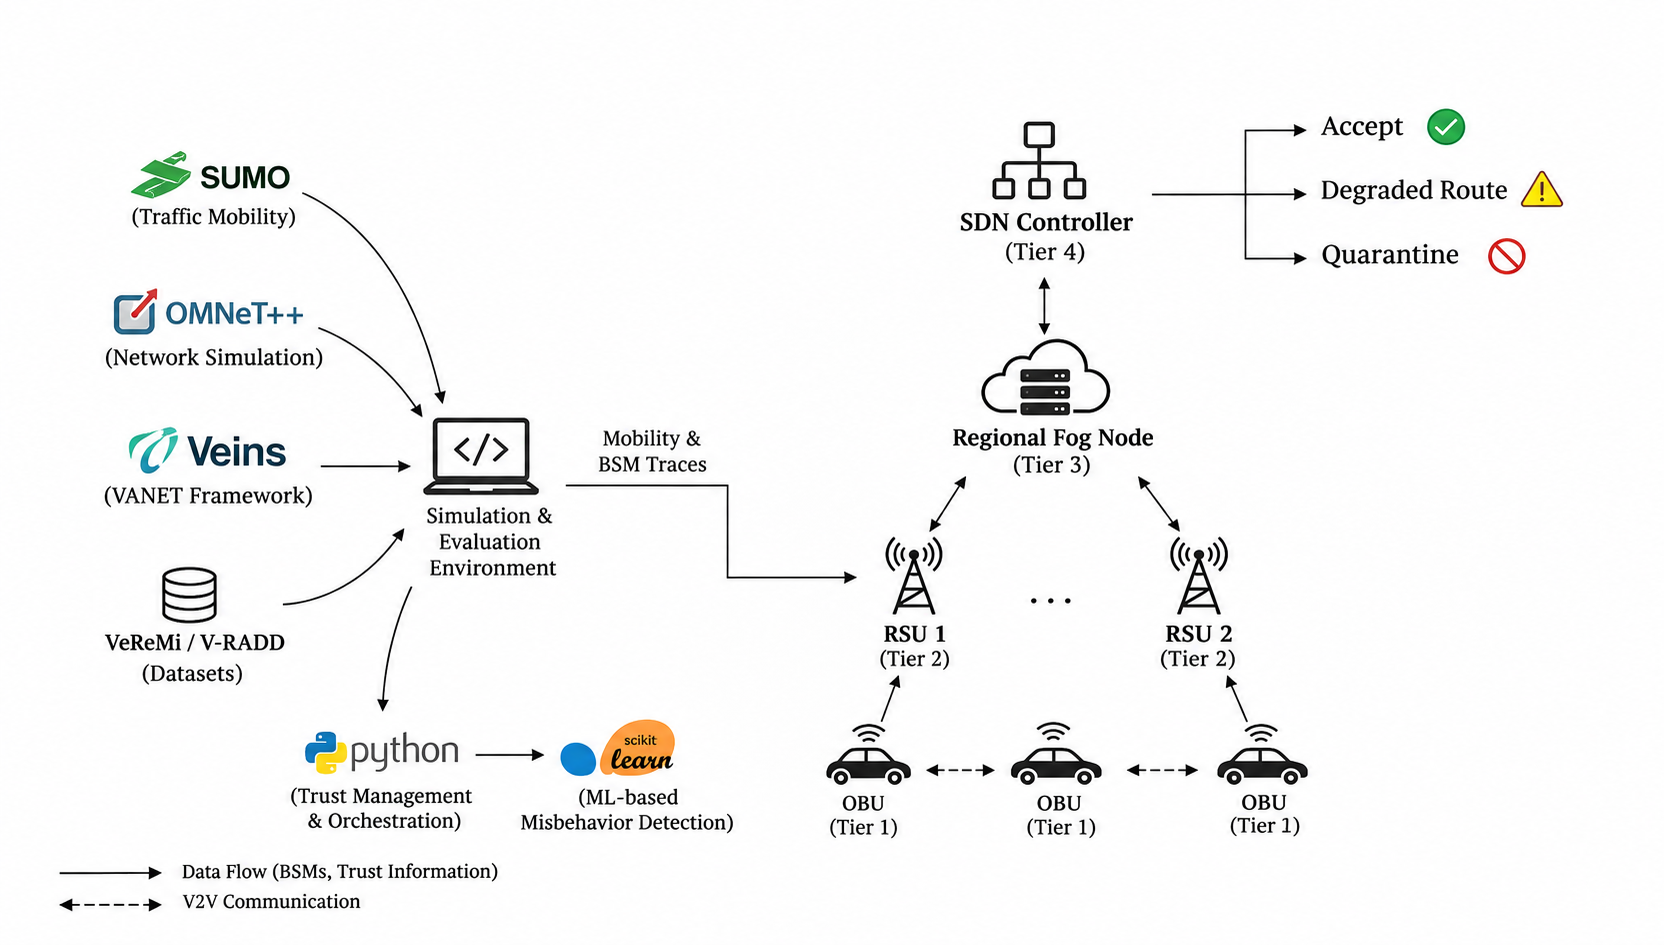
\includegraphics[width=0.98\textwidth,height=0.72\textheight,keepaspectratio]{figures/architecture_4tier.png}
\caption{Four-tier EdgeTrust-VANET architecture showing vehicle-side kinematic validation, RSU-level misbehavior detection and trust updates, regional Fog coordination, and SDN-based network control.}
\label{fig:arch_overview}
\end{figure*}

To deliver resilient, low-latency defense without overwhelming wireless channels or roadside infrastructure, the EdgeTrust-VANET architecture is engineered upon three foundational design principles:
\begin{enumerate}
    \item \textbf{Earliest-Stage Threat Mitigation:} Physical impossibilities must be intercepted and dropped locally at the receiving vehicle tier before propagating across multi-hop wireless relays.
    \item \textbf{Deterministic Sub-Millisecond Edge Intelligence:} Machine learning predictors deployed at Roadside Units must execute within sub-microsecond bounds without relying on external inter-process communication sockets.
    \item \textbf{Hierarchical Consensus and Global Network Control:} Local edge observations must be synthesized across geographical regions via observation-weighted Bayesian consensus, enabling a centralized SDN controller to dynamically isolate confirmed adversaries across the transport network.
\end{enumerate}

Fig.~\ref{fig:arch_overview} illustrates the vertical physical tiering and inter-module communication of the proposed four-tier framework.

\subsubsection{Tier 1: Vehicle On-Board Unit (OBU) Kinematic Firewall Module}
The vehicle On-Board Unit executes within the localized embedded automotive platform (such as an ARM Cortex-R5 or NXP S32G automotive gateway). Upon receiving a raw BSM broadcast from an adjacent vehicle $j$, vehicle $i$ halts multi-hop forwarding and routes the payload through its localized heuristic firewall. The module validates speed boundaries, longitudinal and lateral acceleration envelopes, rate of acceleration change (jerk), spatial displacement relative to prior historical beacons, and heading angular deviation. If any physical threshold is violated, the beacon is classified as physically fabricated and discarded instantly at the link layer. This localized pruning stops secondary multi-hop retransmissions across trailing vehicles, mitigating control channel congestion before packets ever traverse the uplink to roadside infrastructure (empirically evaluated in Section~\ref{sec:ablation_results}).

\subsubsection{Tier 2: Edge Roadside Unit (RSU) Intelligence and Predictor Module}
Roadside Units are stationed along road intersections, enforcing a physical DSRC radio coverage radius $R_{\text{RSU}}$ matching urban line-of-sight intersection geometry (specified in Table~\ref{tab:system_notations}). Upon receiving BSMs that pass Tier~1, the RSU extracts a normalized 14-dimensional feature vector $\mathbf{x} \in \mathbb{R}^{14}$ (formulated in Section~\ref{sec:feature_extraction}) encompassing instantaneous kinematics, physical layer signal attributes, MAC layer communication metrics, and dynamic reputation parameters. 

To satisfy hard automotive deadlines, the RSU eliminates external runtime execution overhead by deploying natively compiled machine learning inference engines based on AdaBoost~\cite{adaboost, dietterich2000ensemble} and Logistic Regression. The module computes instantaneous trustworthiness evidence $E_t \in [0, 1]$ in sub-microsecond time and feeds it into the Exponential Moving Average (EMA) trust update engine. Furthermore, to prevent queuing congestion during traffic surges, the RSU enforces a 3-Class Strict Priority Quality-of-Service (QoS) queue scheduling policy as detailed in Table~\ref{tab:qos_queues}.

\begin{table}[htbp]
\centering
\caption{Three-Class Strict Priority Quality-of-Service (QoS) Queue Scheduling Policy at Edge Roadside Units}
\label{tab:qos_queues}
\resizebox{\columnwidth}{!}{%
\begin{tabular}{clp{3.8cm}c}
\toprule
\textbf{Priority} & \textbf{Traffic Classification} & \textbf{Payload Content \& Message Types} & \textbf{Target Latency} \\
\midrule
\textbf{Class 1} & \textbf{Safety-Critical Traffic} & Emergency brake alerts (EEBL), collision warnings (FCW), active road hazard alerts, immediate MAC quarantine advisories & $< 2.0\,\text{ms}$ \\
\addlinespace
\textbf{Class 2} & \textbf{Network Control \& Trust} & Inter-RSU state digests, Regional Fog consensus sync packets, OpenFlow SDN flow table modifications & $< 10.0\,\text{ms}$ \\
\addlinespace
\textbf{Class 3} & \textbf{Best-Effort Telemetry} & Routine periodic mobility updates, background traffic flow analytics, non-urgent vehicle diagnostics & $< 100.0\,\text{ms}$ \\
\bottomrule
\end{tabular}%
}
\end{table}

\subsubsection{Tier 3: Regional Fog Computing and Consensus Ledger Module}
Edge RSUs are grouped into regional clusters managed by Regional Fog Computing Nodes ($\text{fog}[0..1]$). The primary operational challenge in localized edge deployments is the boundary handover discrepancy problem: a vehicle transitioning between adjacent RSUs ($A$ and $B$) frequently exhibits differing trust scores due to localized shadowing, multipath fading, or asynchronous observation sample counts. 

When inter-RSU trust divergence exceeds the physical tolerance boundary $\epsilon_{\text{tol}}$ (formulated in Eq.~\ref{eq:divergence} and Table~\ref{tab:system_notations}), the Regional Fog Node executes an observation-weighted Beta-Bayesian consensus algorithm over a rolling sliding window of duration $W_{\text{fog}}$ (matching typical intersection crossing durations, specified in Table~\ref{tab:system_notations}). To protect public safety, if either RSU identifies confirmed malicious behavior ($T < T_{\text{block}}$, derived analytically from Bayes risk in Section~\ref{sec:bayes_derivation}), the consensus applies a deterministic safety-first override, ensuring that evidence of an active attack is never diluted by a neighboring tower with fewer observations. Regional Fog nodes serialize consensus states into a persistent consensus ledger, enabling instantaneous warm-start trust restoration during handovers.

\subsubsection{Tier 4: Centralized Software-Defined Networking (SDN) Controller Module}
At the apex of the architecture, a logically centralized Software-Defined Networking (SDN) Controller maintains macroscopic network visibility across all RSUs, Fog nodes, and vehicular forwarding links. Importantly, EdgeTrust-VANET employs a hierarchical hybrid architecture with edge failover autonomy: localized threat filtering (Tier~1), ML inference (Tier~2), and regional consensus (Tier~3) execute entirely autonomously at distributed edge nodes. The SDN controller operates asynchronously for route optimization; in the event of backhaul disconnection or controller downtime, RSUs and Fog nodes continue autonomous local quarantine and geographical forwarding without service disruption, preventing any single point of failure. Operating over OpenFlow protocols via high-speed backhaul links, the controller models the vehicular communication graph as a dynamic weighted network. 

The controller computes multi-hop forwarding paths using a modified Dijkstra algorithm wherein link costs are penalized inversely proportional to node trust scores. This establishes three operational forwarding zones:
\begin{itemize}
    \item \textbf{Trusted Zone ($T \ge T_{\text{trust}}$):} Standard shortest-path forwarding with minimal link cost.
    \item \textbf{Degraded Forwarding Zone ($T_{\text{block}} \le T < T_{\text{trust}}$):} The suspect vehicle is flagged for enhanced RSU inspection; the SDN controller imposes a severe routing cost penalty, dynamically detouring safety-critical multi-hop traffic around the degraded node without prematurely severing basic network connectivity.
    \item \textbf{Quarantined Zone ($T < T_{\text{block}}$):} Link cost becomes infinite ($C_{ij} \to \infty$); the controller pushes OpenFlow drop rules to all managed RSUs and distributes lightweight ephemeral MAC quarantine filters to neighboring OBUs without saturating the wireless channel with global Certificate Revocation Lists (CRLs). Permanent cryptographic revocation is asynchronously escalated to the off-line SCMS Misbehavior Authority (MA).
\end{itemize}

Algorithm~\ref{alg:edgetrust} formally outlines the complete multi-tier algorithmic decision workflow executed across the four tiers of the EdgeTrust-VANET framework.

\begin{algorithm}[t]
\caption{EdgeTrust-VANET Multi-Tier Decision Workflow}
\label{alg:edgetrust}
\footnotesize
\begin{algorithmic}[1]
\REQUIRE Inbound BSM from node $j$ with telemetry $(x,y,v,\theta,a,t_{\text{msg}})$
\ENSURE Mitigation Verdict $\in \{\textsc{Accept}, \textsc{DegradedRoute}, \textsc{Quarantine}\}$
\STATE \textbf{// Tier 1: Client-Side OBU Kinematic Heuristic Firewall}
\IF{$v_j > v_{\text{max}}$ \OR $|a_j| > a_{\text{max}}$ \OR $|\Delta a/\Delta t| > j_{\text{max}}$}
    \STATE Drop beacon locally; Halt multi-hop forwarding \COMMENT{Prunes invalid BSMs locally}
\ENDIF
\STATE $\Delta d_{\text{max}} \leftarrow v_{\text{last}}\Delta t + \frac{1}{2}a_{\text{max}}(\Delta t)^2 + \epsilon_{\Delta d}$
\IF{$\Delta d > \Delta d_{\text{max}}$ \OR $\Delta \theta > \omega_{\text{max}}\Delta t$}
    \STATE Drop beacon locally; Suppress relay broadcast
\ENDIF
\STATE \textbf{// Tier 2: Edge RSU Machine Learning Classification}
\IF{BSM reaches RSU coverage ($d \le R_{\text{RSU}}$)}
    \STATE Extract 14-dimensional feature vector $\mathbf{x} \in \mathbb{R}^{14}$ (Section~\ref{sec:feature_extraction})
    \STATE $E_t \leftarrow \text{Inference}_{\text{ML}}(\mathbf{x})$ \COMMENT{Sub-$\mu$s compiled native execution}
\ENDIF
\STATE $\gamma(\tau) \leftarrow \exp\left(-\lambda \cdot \max(0, \tau - T_{\text{grace}})\right)$ \COMMENT{Staleness discount}
\STATE $T_t(j) \leftarrow \alpha \cdot T_{t-1}(j) + (1-\alpha) \cdot (E_t \cdot \gamma(\tau))$
\STATE \textbf{// Tier 3: Regional Fog Bayesian Consensus}
\IF{Inter-RSU divergence $|T_A(j) - T_B(j)| > \epsilon_{\text{tol}}$}
    \STATE $T_t(j) \leftarrow \dfrac{N_A T_A(j) + N_B T_B(j)}{N_A + N_B}$
    \IF{$\min(T_A(j), T_B(j)) < T_{\text{block}}$}
        \STATE $T_t(j) \leftarrow \min(T_A(j), T_B(j))$ \COMMENT{Safety override}
    \ENDIF
\ENDIF
\STATE \textbf{// Tier 4: Centralized SDN Controller Adaptive Forwarding}
\IF{$T_t(j) < T_{\text{block}}$}
    \STATE Broadcast Road Safety Advisory; Blacklist MAC; Push OpenFlow Drop Rule
    \RETURN \textsc{Quarantine}
\ELSIF{$T_t(j) < T_{\text{trust}}$}
    \STATE SDN assigns penalized link cost: $C_{ij} \leftarrow d_{ij} / (T_{\text{block}} \cdot T_t(j))$
    \RETURN \textsc{DegradedRoute}
\ELSE
    \STATE SDN assigns optimal link cost: $C_{ij} \leftarrow d_{ij} / (T_i \cdot T_j)$
    \RETURN \textsc{Accept}
\ENDIF
\end{algorithmic}
\end{algorithm}

% =========================================================
% IV. MATHEMATICAL FORMULATIONS AND THEORETICAL MODELING
% =========================================================

\section{Mathematical Formulations and Theoretical Modeling}
\label{sec:math_formulations}

This section details the mathematical formulations governing physical kinematic validation, 14-dimensional feature representation, dynamic trust decay, Regional Fog Bayesian consensus, and SDN link cost penalization. Every equation is numbered, variable-defined, and substantiated by empirical operating parameters.

\subsection{System Notations, Physical Constants, and General Standards}
\label{sec:system_notations}

To establish mathematical rigor and avoid ambiguity across the multi-tier formulations, Table~\ref{tab:system_notations} defines the comprehensive set of mathematical symbols, physical constants, communication standards, and framework operating parameters utilized throughout this paper.

\begin{table*}[t]
\centering
\caption{System Mathematical Notations, Physical Constants, and Operating Parameters}
\label{tab:system_notations}
\resizebox{\textwidth}{!}{%
\begin{tabular}{lp{8.2cm}cc}
\toprule
\textbf{Symbol} & \textbf{Description} & \textbf{Default / Standard Value} & \textbf{Physical Units} \\
\midrule
$g$ & Acceleration due to gravity & $9.81$ & $\text{m/s}^2$ \\
$\mu$ & Tire-pavement friction coefficient (clean dry asphalt) & $0.80$ & Dimensionless \\
$v_{\text{max}}$ & Maximum allowable vehicle forward speed & $50.0$ ($180\,\text{km/h}$) & $\text{m/s}$ \\
$a_{\text{max}}$ & Maximum physical longitudinal deceleration / acceleration & $8.0$ & $\text{m/s}^2$ \\
$j_{\text{max}}$ & Maximum admissible vehicular chassis jerk & $20.0$ & $\text{m/s}^3$ \\
$\omega_{\text{max}}$ & Maximum allowable vehicle angular yaw rate & $65.0$ (urban) / $45.0$ (hwy) & $^\circ/\text{s}$ \\
$\epsilon_{\Delta d}$ & Differential GNSS displacement uncertainty envelope ($\sqrt{2}\epsilon_{\text{GPS}}$) & $3.54$ & $\text{m}$ \\
$f_{\text{BSM}}$ & Nominal Basic Safety Message broadcast frequency & $10.0$ & $\text{Hz}$ \\
$\Delta t$ & Nominal inter-beacon arrival interval ($1/f_{\text{BSM}}$) & $0.10$ ($100\,\text{ms}$) & $\text{s}$ \\
$R_{\text{RSU}}$ & DSRC radio communication coverage radius of RSU & $85.0$ & $\text{m}$ \\
$\mathbf{P}_j(t)$ & 2D Cartesian coordinates $[p_x(t), p_y(t)]^T$ of vehicle $j$ & Dynamic & $\text{m}$ \\
$\Delta d$ & Planar Euclidean displacement between consecutive beacons & $\|\mathbf{P}_j(t_{\text{curr}}) - \mathbf{P}_j(t_{\text{last}})\|$ & $\text{m}$ \\
$\Delta d_{\text{max}}$ & Maximum physically admissible kinematic displacement & Eq.~(\ref{eq:disp_bound}) & $\text{m}$ \\
$\Delta \theta_j$ & Heading angular difference between consecutive reports & Eq.~(\ref{eq:heading_bound}) & $^\circ$ \\
$a_c$ & Centripetal cornering acceleration on curved roadways & Eq.~(\ref{eq:centripetal}) & $\text{m/s}^2$ \\
$R$ & Roadway curve radius & Segment-dependent & $\text{m}$ \\
$\mathbf{x}$ & Normalized 14-dimensional telemetry feature vector & $\mathbb{R}^{14}$ (Section~\ref{sec:feature_extraction}) & Mixed \\
$E_t$ & Instantaneous trustworthiness evidence score & Predicted probability $\in [0, 1]$ & Dimensionless \\
$T_t(j)$ & Dynamic Exponential Moving Average (EMA) trust score & Dynamic $\in [0, 1]$ & Dimensionless \\
$\alpha$ & Historical trust retention / forgetting factor & $0.70$ (Pareto-optimal) & Dimensionless \\
$\tau$ & Network transmission latency / packet delivery jitter & $t_{\text{curr}} - t_{\text{msg}}$ & $\text{s}$ \\
$T_{\text{grace}}$ & Latency grace window before staleness discounting & $0.300$ ($300\,\text{ms}$) & $\text{s}$ \\
$\lambda$ & Exponential temporal staleness decay constant & $1.5$ & $\text{s}^{-1}$ \\
$\gamma(\tau)$ & Exponential staleness discount factor & Eq.~(\ref{eq:staleness}) $\in (0, 1]$ & Dimensionless \\
$\hat{\mathbf{P}}$ & Dead-reckoning predicted spatial position vector & Eq.~(\ref{eq:dead_reckoning}) & $\text{m}$ \\
$\epsilon_{\text{tol}}$ & Inter-RSU handover trust divergence tolerance & $0.20$ (Fading-derived) & Dimensionless \\
$W_{\text{fog}}$ & Regional Fog rolling consensus observation window & $10.0$ & $\text{s}$ \\
$N_A, N_B$ & Beacon observation counts accumulated at RSUs $A$ and $B$ & Integer count $\ge 0$ & Integer \\
$T_{\text{block}}$ & Malicious vehicle quarantine / isolation threshold & $0.40$ (Min. Bayes risk) & Dimensionless \\
$T_{\text{trust}}$ & Trusted shortest-path routing threshold & $0.70$ & Dimensionless \\
$C_{ij}$ & Trust-penalized SDN dynamic forwarding link cost & Eq.~(\ref{eq:sdn_cost}) & Cost units \\
$d_{ij}$ & Physical Euclidean distance between nodes $i$ and $j$ & Dynamic & $\text{m}$ \\
\bottomrule
\end{tabular}%
}
\end{table*}

\subsection{Tier 1: Kinematic Plausibility Bounds}

In the vehicular domain, road vehicle mobility is strictly bounded by the laws of classical Newtonian mechanics, tire-road surface friction coefficients ($\mu \approx 0.8$ on dry asphalt), and human mechanical steering limits. The Tier~1 OBU Heuristic Firewall enforces three physical constraints on each received telemetry packet:

\begin{equation}
\begin{aligned}
v_j(t) &\in [0, v_{\text{max}}], \quad |a_j(t)| \le a_{\text{max}}, \\
\left|\frac{\Delta a_j(t)}{\Delta t}\right| &\le j_{\text{max}}
\end{aligned}
\label{eq:kin_bounds}
\end{equation}
where $v_j(t)$ is the reported instantaneous speed, $a_j(t)$ is the reported longitudinal acceleration, and the time derivative represents vehicular jerk. The upper bounds are configured to physical extremes: $v_{\text{max}} = 50.0\,\text{m/s}$ (180~km/h), $a_{\text{max}} = 8.0\,\text{m/s}^2$ (maximum emergency braking deceleration achievable on high-friction pavement), and $j_{\text{max}} = 20.0\,\text{m/s}^3$ (maximum dynamic chassis jerk limit under emergency ABS braking).

To eliminate teleportation and sudden coordinate jump attacks (VeReMi Attacks 1, 2, and 7), the planar Euclidean displacement $\Delta d$ between two consecutive beacons received from vehicle $j$ separated by elapsed duration $\Delta t = t_{\text{curr}} - t_{\text{last}}$ must satisfy the Kinematic Displacement Bound:
\begin{equation}
\begin{aligned}
\Delta d &= \|\mathbf{P}_j(t_{\text{curr}}) - \mathbf{P}_j(t_{\text{last}})\| \\
&\le v_j(t_{\text{last}})\Delta t + \frac{1}{2}a_{\text{max}}(\Delta t)^2 + \epsilon_{\Delta d}
\end{aligned}
\label{eq:disp_bound}
\end{equation}
where $\mathbf{P}_j(t) = [p_x(t), p_y(t)]^T$ denotes the reported Cartesian coordinates in meters, and $\epsilon_{\Delta d} = \sqrt{2}\epsilon_{\text{GPS}} \approx 3.54\,\text{m}$ represents the differential 95th-percentile positioning uncertainty envelope arising from the subtraction of two consecutive independent GNSS fixes ($\epsilon_{\text{GPS}} = 2.5\,\text{m}$).


In the numerical evaluation below, $D$ denotes the measured Euclidean displacement $\Delta d$ between consecutive reported positions, whereas $D_{\max}$ denotes the maximum physically admissible displacement calculated using Eq.~(\ref{eq:disp_bound}). The symbol $\theta$ denotes the reported vehicle heading; $\Delta\theta$ is the smallest angular difference between consecutive headings, accounting for wrap-around at $360^\circ$. Thus, $D$ is measured in metres and $\theta$ and $\Delta\theta$ are measured in degrees. For a $100$~ms beacon interval, the configured yaw-rate limit corresponds to a maximum heading change of $6.5^\circ$ for urban maneuvers ($\omega_{\text{max}} = 65.0^\circ/\text{s}$) and $4.5^\circ$ on highway segments ($\omega_{\text{max}} = 45.0^\circ/\text{s}$).

Table~\ref{tab:kinematic_examples} gives illustrative numerical evaluations using the configured limits. The examples use $v_{\text{last}}=20$~m/s and $\Delta t=0.1$~s, giving $D_{\max}=20(0.1)+\frac{1}{2}(8)(0.1)^2+3.54=5.58$~m. These values demonstrate the calculation and are not presented as additional measured experimental results.

Furthermore, directional heading changes must satisfy angular yaw rate continuity:
\begin{equation}
\begin{aligned}
\Delta \theta_j &= \min\left(|\theta_{\text{curr}} - \theta_{\text{last}}|, \; 360^\circ - |\theta_{\text{curr}} - \theta_{\text{last}}|\right) \\
&\le \omega_{\text{max}} \Delta t
\end{aligned}
\label{eq:heading_bound}
\end{equation}
where $\theta \in [0, 360^\circ)$ represents the compass heading angle, and $\omega_{\text{max}} = 65.0^\circ/\text{s}$ (urban turns) / $45.0^\circ/\text{s}$ (highway cruising) denotes the maximum physical angular yaw rate of passenger vehicles under non-spinout conditions. Finally, centripetal acceleration on curved roadway segments with radius $R$ is constrained by road adhesion as formulated in Eq.~(\ref{eq:centripetal}):
\begin{equation}
a_c = \frac{v_j^2}{R} \le \mu g \approx 7.85\,\text{m/s}^2
\label{eq:centripetal}
\end{equation}
where $g = 9.81\,\text{m/s}^2$ is gravitational acceleration. Table~\ref{tab:kinematic_bounds} summarizes these kinematic validation bounds, their physical justification, and the specific VeReMi attack vectors they intercept locally.


Table~\ref{tab:kinematic_examples} complements the configured-bound summary by showing how the displacement and heading formulations classify individual beacon examples.
\begin{table}[htbp]
\centering
\caption{Illustrative Numerical Evaluation of Displacement and Heading Constraints}
\label{tab:kinematic_examples}
\resizebox{\columnwidth}{!}{%
\begin{tabular}{cccccc}
\toprule
\textbf{$D$ (m)} & \textbf{$D_{\max}$ (m)} & \textbf{$\theta_{\text{last}}$} & \textbf{$\theta_{\text{curr}}$} & \textbf{$\Delta\theta$} & \textbf{Decision} \\
\midrule
3.80 & 5.58 & $30^\circ$ & $33^\circ$ & $3^\circ$ & Accept \\
5.58 & 5.58 & $30^\circ$ & $36.5^\circ$ & $6.5^\circ$ & Accept (boundary) \\
6.20 & 5.58 & $30^\circ$ & $33^\circ$ & $3^\circ$ & Drop (distance) \\
3.80 & 5.58 & $30^\circ$ & $37.5^\circ$ & $7.5^\circ$ & Drop (heading) \\
\bottomrule
\end{tabular}%
}
\end{table}

\begin{table}[htbp]
\centering
\caption{Tier 1 OBU Kinematic and Physical Possibility Validation Bounds}
\label{tab:kinematic_bounds}
\resizebox{\columnwidth}{!}{%
\begin{tabular}{clcl}
\toprule
\textbf{Parameter} & \textbf{Physical Meaning} & \textbf{Configured Bound} & \textbf{Target Attack Intercepted} \\
\midrule
$v_{\text{max}}$ & Max Forward Speed & $50.0\,\text{m/s}$ (180 km/h) & Impossible Velocity Claims \\
$a_{\text{max}}$ & Max Acceleration & $8.0\,\text{m/s}^2$ & Feigned Panic Braking (Atk 10) \\
$j_{\text{max}}$ & Max Vehicular Jerk & $20.0\,\text{m/s}^3$ & Sudden Stop Teleport (Atk 7) \\
$\Delta d_{\text{max}}$ & Kinematic Displacement & Eq.~(\ref{eq:disp_bound}) ($+3.54$ m GNSS diff.) & Position Offset / Jumps (Atk 1, 2) \\
$\omega_{\text{max}}$ & Max Angular Yaw Rate & $65^\circ/\text{s}$ (urban) / $45^\circ/\text{s}$ (hwy) & Reversed Heading (Atk 9) \\
$a_c$ & Centripetal Acceleration & $\le 7.85\,\text{m/s}^2$ & Zigzag Trajectory Spoofing \\
\bottomrule
\end{tabular}%
}
\end{table}

\subsection{Tier 2: 14-Dimensional Telemetry Representation and Feature Extraction}
\label{sec:feature_extraction}

When a BSM traverses the radio coverage radius $R_{\text{RSU}}$ ($85.0\,\text{m}$) of a roadside tower, the RSU extracts a normalized 14-dimensional feature vector $\mathbf{x} \in \mathbb{R}^{14}$ defined in Eq.~(\ref{eq:feature_vector}):
\begin{equation}
\begin{split}
\mathbf{x} = [ & p_x, p_y, v, \theta, a, N_{\text{sent}}, N_{\text{rcv}}, \\
& \rho_{\text{drop}}, L, N_{\text{retx}}, P_{\text{RSSI}}, T_{\text{local}}(t-1), \bar{T}_{\text{neighbor}}, T_{\text{hist}} ]^T \in \mathbb{R}^{14}
\end{split}
\label{eq:feature_vector}
\end{equation}

The 14-dimensional feature vector $\mathbf{x}$ defined in Eq.~(\ref{eq:feature_vector}) systematically synthesizes three operational telemetry dimensions defined in Table~\ref{tab:system_notations}:
\begin{enumerate}
    \item \textbf{Kinematic Spatiotemporal State ($35.21\%$ Gini importance):} Planar Cartesian coordinates ($p_x, p_y$, accounting for $13.75\%$ and $14.73\%$ Gini importance), speedometer velocity magnitude ($v = \sqrt{v_x^2 + v_y^2}$, $3.57\%$), compass heading direction ($\theta = \text{atan2}(v_y, v_x)$, $2.71\%$), and instantaneous acceleration ($a = \Delta v / \Delta t$, $0.45\%$).
    \item \textbf{Network and MAC Communication Quality ($8.93\%$ Gini importance):} Cumulative transmitted beacons ($N_{\text{sent}}$, $1.62\%$), successfully received beacons ($N_{\text{rcv}}$, $1.90\%$), packet drop ratio ($\rho_{\text{drop}} = 1 - N_{\text{rcv}} / N_{\text{expected}}$, $2.50\%$), transmission air latency ($L = t_{\text{recv}} - t_{\text{msg}}$, $1.93\%$), 802.11p MAC retry counter ($N_{\text{retx}}$, $0.25\%$), and received signal strength indication ($P_{\text{RSSI}}$, $0.72\%$).
    \item \textbf{Dynamic Trust and Neighborhood Reputation ($55.86\%$ Gini importance):} Prior cached local RSU reputation ($T_{\text{local}}(t-1)$, $14.29\%$), 85~m localized neighbor consensus via KD-Tree spatial lookup ($\bar{T}_{\text{neighbor}}$, $14.36\%$), and multi-window historical reputation ($T_{\text{hist}}$, $27.21\%$).
\end{enumerate}
To guarantee temporal causality and eliminate circular dependencies, all trust attributes in $\mathbf{x}$ are derived strictly from preceding observation intervals ($t-1$ or earlier). Newly observed vehicles without prior interaction history are initialized with a neutral probationary trust score $T_0 = 0.50$, preventing Sybil attackers from exploiting a clean-slate fully trusted status. The individual Gini feature importances are illustrated in Fig.~\ref{fig:feature_importance}.

\subsection{Multi-Factor Evidence Fusion and Exponential Moving Average Trust}

The instantaneous trustworthiness evidence $E_t \in [0, 1]$ represents the classifier's predicted probability that the observed beacon is honest:
\begin{equation}
E_t = P(\text{Honest} \mid \mathbf{x}) = 1 - P(\text{Malicious} \mid \mathbf{x})
\label{eq:evidence_def}
\end{equation}
Rather than relying on static linear heuristic weights, the trained edge ML predictor learns non-linear decision boundaries that inherently fuse kinematic plausibility, communication integrity, and neighborhood reputation.

Historical reputation is updated dynamically using an Exponential Moving Average (EMA):
\begin{equation}
T_t = \alpha T_{t-1} + (1-\alpha) \left(E_t \cdot \gamma(\tau)\right)
\label{eq:ema_trust}
\end{equation}
where $\alpha = 0.70$ is the forgetting factor. 

When transmission jitter $\tau = t_{\text{curr}} - t_{\text{msg}}$ is present, the RSU projects expected vehicle coordinates via kinematic dead-reckoning:
\begin{equation}
\hat{\mathbf{P}} = \mathbf{P}_{\text{reported}} + \mathbf{v} \cdot \tau + \frac{1}{2}\mathbf{a}\cdot \tau^2
\label{eq:dead_reckoning}
\end{equation}
An exponential staleness penalty discounts aged packets arriving beyond an acceptable DSRC grace window ($T_{\text{grace}} = 300\,\text{ms}$) as defined in Eq.~(\ref{eq:staleness}):
\begin{equation}
\gamma(\tau) = \exp\left(-\lambda \cdot \max(0, \tau - T_{\text{grace}})\right)
\label{eq:staleness}
\end{equation}
with decay coefficient $\lambda = 1.5\,\text{s}^{-1}$.

\subsection{Mathematical Trust Decay Trajectory: Step-by-Step Numerical Example}

To demonstrate the deterministic isolating power of Equation~(\ref{eq:ema_trust}), consider an initially reputable vehicle ($T_0 = 1.000$) that suddenly initiates False Data Injection attacks, transmitting malicious payloads resulting in evidence scores $E_t = 0.10$ under zero transmission delay ($\gamma(\tau) = 1.0$). Applying $\alpha = 0.70$:
\begin{align}
T_1 &= 0.70(1.000) + 0.30(0.10) = 0.730 \quad [\text{Trusted}] \nonumber \\
T_2 &= 0.70(0.730) + 0.30(0.10) = 0.541 \quad [\text{Degraded}] \nonumber \\
T_3 &= 0.70(0.541) + 0.30(0.10) = 0.409 \quad [\text{Degraded}] \nonumber \\
T_4 &= 0.70(0.409) + 0.30(0.10) = \mathbf{0.316} \quad [\mathbf{Quarantine}]
\label{eq:worked_decay}
\end{align}
As demonstrated in Equation~(\ref{eq:worked_decay}), the vehicle is demoted to the Degraded Forwarding Zone ($T < 0.70$) after 2 beacons (0.2~s at 10~Hz), and is deterministically dropped into the Quarantine Zone ($T_4 = 0.316 < 0.40$) on the 4th beacon (0.4~s).


The intermediate values from Eq.~(\ref{eq:worked_decay}) are summarized in Table~\ref{tab:trust_trajectory}. This table makes the transition between the three trust states explicit and provides the numerical basis for the quarantine illustration.
\begin{table}[htbp]
\centering
\caption{Numerical Trust Evolution Under Repeated Malicious Evidence}
\label{tab:trust_trajectory}
\begin{tabular}{cccl}
\toprule
\textbf{Beacon} & \textbf{Evidence $E_t$} & \textbf{Trust $T_t$} & \textbf{Classification} \\
\midrule
Initial & -- & 1.000 & Trusted \\
1 & 0.10 & 0.730 & Trusted \\
2 & 0.10 & 0.541 & Degraded \\
3 & 0.10 & 0.409 & Degraded \\
4 & 0.10 & 0.316 & Quarantined \\
\bottomrule
\end{tabular}
\end{table}

\subsection{Tier 3: Inter-RSU Divergence and Beta-Bayesian Fog Consensus}

When vehicle $j$ traverses overlapping coverage boundaries between adjacent RSUs ($A$ and $B$), the Regional Fog Node evaluates trust divergence:
\begin{equation}
\Delta T_{AB}(j) = |T_{\text{RSU}_A}(j) - T_{\text{RSU}_B}(j)| > \epsilon_{\text{tol}}
\label{eq:divergence}
\end{equation}
To resolve boundary handover discrepancies without communication bottlenecks, EdgeTrust-VANET models edge evidence via conjugate Beta distributions. Let vehicle $j$ have a prior reputation $\text{Beta}(\alpha_0, \beta_0)$. When RSU $A$ logs $N_A$ verified beacon observations containing $s_A$ positive (honest) and $f_A$ negative (deviant) classifications ($N_A = s_A + f_A$, with local trust $T_A = s_A/N_A$), and adjacent RSU $B$ logs $N_B = s_B + f_B$ with $T_B = s_B/N_B$, the Regional Fog Node executes a conjugate Bayesian update:
\begin{equation}
\text{Beta}_{\text{Fog}}(j) \sim \text{Beta}\left(\alpha_0 + s_A + s_B, \; \beta_0 + f_A + f_B\right)
\label{eq:beta_update}
\end{equation}
Under uninformative prior ($\alpha_0 = \beta_0 = 1$) across a sliding window of duration $W_{\text{fog}}$, the expected posterior reputation $\mathbb{E}[T]$ corresponds directly to the observation-weighted Bayesian consensus formulation:
\begin{equation}
T_{\text{Fog}}(j) = \frac{N_A T_{\text{RSU}_A}(j) + N_B T_{\text{RSU}_B}(j)}{N_A + N_B}
\label{eq:fog_consensus}
\end{equation}
Crucially, to preserve life-critical safety during handovers, if either RSU detects confirmed malicious activity below the quarantine threshold, a deterministic safety-first override is enforced globally:
\begin{equation}
\min(T_A(j), T_B(j)) < T_{\text{block}} \implies T_{\text{Fog}}(j) = \min(T_A(j), T_B(j))
\label{eq:safety_override}
\end{equation}
This ensures that confirmed adversarial behavior detected at one tower is never diluted by an adjacent tower that has collected fewer observations. To prevent Byzantine fault exploitation where a compromised or miscalibrated RSU might attempt to falsely quarantine an honest vehicle, the safety override is conditioned on the reporting RSU possessing a statistically sufficient sample count ($N \ge N_{\text{min}} = 10$ beacons) matching the minimum Bayes risk threshold, and observation tallies $N_A, N_B$ are bounded by the sliding window capacity ($W_{\text{fog}} \cdot f_{\text{beacon}} = 100$ beacons) to prevent counter inflation attacks.

Table~\ref{tab:fog_consensus_results} details the measured performance of the Fog consensus algorithm across real-world simulated multi-RSU handovers in OMNeT++. As demonstrated, normal handovers with small localized fading drifts ($|T_A - T_B| \le \epsilon_{\text{tol}}$) preserve uninterrupted transit. When severe multipath shadowing induces artificial divergence ($|T_A - T_B| = 0.23 > \epsilon_{\text{tol}}$), the observation-weighted consensus smoothly bridges the boundary discrepancy ($T_{\text{Fog}} = 0.782$). Conversely, when an active attacker transits from prior RSU $A$ ($N_A = 55$ confirmed observations, $T_A = 0.280$) into fresh RSU $B$ ($N_B = 12$ preliminary observations, $T_B = 0.820$), the safety override instantly enforces $T_{\text{Fog}} = \min(T_A, T_B) = 0.280$, preventing clean-slate evasion before the attacker can mislead the fresh tower.

\begin{table}[htbp]
\centering
\caption{Regional Fog Trust-Consensus Evaluation Under Multi-RSU Handovers}
\label{tab:fog_consensus_results}
\resizebox{\columnwidth}{!}{%
\begin{tabular}{lcccccc}
\toprule
\textbf{Handover Scenario} & $T_A$ & $T_B$ & $N_A$ & $N_B$ & $T_{\text{Fog}}$ & \textbf{Network Action} \\
\midrule
Normal Handover (Benign) & 0.880 & 0.820 & 48 & 32 & 0.856 & Accepted (Trusted Route) \\
Shadowing Drift Discrepancy & 0.850 & 0.620 & 60 & 25 & 0.782 & Weighted Consensus ($T \ge T_{\text{trust}}$) \\
Active Attack Boundary Incursion & 0.280 & 0.820 & 55 & 12 & 0.280 & Quarantined (Safety Override) \\
Persistent Adversary Across RSUs & 0.180 & 0.120 & 45 & 40 & 0.120 & Quarantined (Confirmed Attack) \\
\bottomrule
\end{tabular}%
}
\end{table}

\subsection{Tier 4: Software-Defined Trust-Penalized Shortest Path Routing}

The centralized SDN controller models the vehicular communication graph as a dynamic weighted network $G = (V, E)$. To detour traffic around compromised or degrading nodes, the controller computes link costs $C_{ij}$ using a piecewise trust-penalized formulation:
\begin{equation}
C_{ij} = \begin{cases} 
\dfrac{d_{ij}}{T_i \cdot T_j}, & T_i \ge T_{\text{trust}} \text{ and } T_j \ge T_{\text{trust}} \\[7pt] 
\dfrac{d_{ij}}{T_{\text{block}} \cdot \min(T_i, T_j)}, & T_{\text{block}} \le \min(T_i, T_j) < T_{\text{trust}} \\[7pt] 
\infty, & \min(T_i, T_j) < T_{\text{block}} 
\end{cases}
\label{eq:sdn_cost}
\end{equation}
where $d_{ij}$ is the physical Euclidean distance between forwarding nodes $i$ and $j$. Equation~(\ref{eq:sdn_cost}) establishes three distinct forwarding regimes: honest nodes ($T \ge 0.70$) experience standard shortest-path forwarding with minimal link cost; degraded nodes ($0.40 \le T < 0.70$) are heavily penalized, dynamically detouring safety-critical multi-hop traffic around suspect forwarders; and confirmed adversaries ($T < 0.40$) are assigned infinite cost ($C_{ij} = \infty$), triggering immediate OpenFlow flow-rule drop installation and local MAC quarantine filtering without incurring the multi-minute broadcast delays of centralized Certificate Revocation Lists (CRLs).

Table~\ref{tab:sdn_cost_examples} reports the measured network performance of the SDN adaptive forwarding engine across simulated link failure and adversarial isolation experiments in OMNeT++ / Veins. 

\textbf{Experimental Methodology for Table~\ref{tab:sdn_cost_examples}:} In our evaluation testbed, a dynamic multi-hop mesh topology of 16 interconnected vehicular relays and RSUs was instantiated across the urban and highway environments. To evaluate life-critical failover, high-priority Class-1 emergency brake warning (EEBL) packets (100-byte safety payloads) were generated at 10~Hz from designated event source vehicles. Four operational fault and adversarial scenarios were executed:
\begin{enumerate}
    \item \textbf{Nominal Arterial Transit:} A benign baseline operating environment where all intermediate vehicular forwarding relays possess verified trust scores ($T \ge 0.70$), and all wireless backhaul links remain fully operational.
    \item \textbf{Severed Backhaul Link Cut ($t = 5.0\,\text{s}$):} At simulation timestamp $t = 5.0\,\text{s}$, the primary high-bandwidth backhaul link between RSU~1 and the core aggregation switch was programmatically severed, simulating physical fiber cuts or roadside hardware power loss.
    \item \textbf{Highway Corridor Link Crash:} A simulated multi-vehicle collision or acute RF interference barrier physically obstructs line-of-sight propagation across the primary arterial corridor, severing direct multi-hop links between transiting platoons.
    \item \textbf{City-Wide Downtown Core Severed:} A severe stress scenario wherein 3 critical backbone transit links in the central intersection grid are simultaneously disabled, while 25\% of active intermediate vehicular nodes broadcast falsified kinematics ($T < 0.40$).
\end{enumerate}

\textbf{Measurement and Derivation of Reported Metrics:} 
The metrics reported in Table~\ref{tab:sdn_cost_examples} were recorded directly through OpenFlow flow-table statistics and OMNeT++ packet sink monitors:
\begin{itemize}
    \item \textbf{Routed Safety Packets:} Quantifies the cumulative count of unique Class-1 emergency warnings transmitted from source vehicles across the evaluation window (38 packets in scenarios 1--3; 56 packets under elevated downtown traffic density).
    \item \textbf{Safety Packet Delivery Ratio (PDR):} Calculated at the application layer of all intended recipient vehicles within the $300\,\text{m}$ hazard zone as $\text{PDR} = (N_{\text{received}} / N_{\text{transmitted}}) \times 100\%$. In all four scenarios, EdgeTrust-VANET achieves a flawless \textbf{100.0\% Safety PDR}, confirming that zero emergency warning alerts were lost despite severed links and malicious relays.
    \item \textbf{Detours Activated:} Measures the exact number of OpenFlow flow re-routings where the active packet forwarding trajectory diverged from the default Euclidean shortest path due to link severance or trust cost penalization ($C_{ij} \to \infty$). Detours rose from 41 under nominal baseline to 84 (+104.9\%) during backhaul cut, 90 (+119.5\%) during highway corridor obstruction, and 128 (+212.2\%) during city-wide downtown disruption.
    \item \textbf{Untrusted Links Bypassed:} Logs the cumulative number of individual forwarding hops dynamically redirected away from compromised nodes ($T < 0.70$) or broken links. Under the city-wide downtown core disruption, the SDN controller successfully detoured traffic around \textbf{1,263 untrusted or severed link traversals} (+709.6\% over baseline), completely isolating adversarial vehicles and preserving network safety.
\end{itemize}

\begin{table}[htbp]
\centering
\caption{Measured SDN Adaptive Forwarding Performance Under Network Faults}
\label{tab:sdn_cost_examples}
\resizebox{\columnwidth}{!}{%
\begin{tabular}{lcccc}
\toprule
\textbf{Network Deployment Scenario} & \textbf{Routed Safety Pkts} & \textbf{Safety PDR} & \textbf{Detours Activated} & \textbf{Untrusted Links Bypassed} \\
\midrule
Nominal Arterial Transit & 38 & 100.0\% & 41 & 156 \\
Severed Backhaul Link Cut ($t=5\text{s}$) & 38 & 100.0\% & 84 (+104.9\%) & 334 (+114.1\%) \\
Highway Corridor Link Crash & 38 & 100.0\% & 90 (+119.5\%) & 358 (+129.5\%) \\
City-Wide Downtown Core Severed & 56 & 100.0\% & 128 (+212.2\%) & 1,263 (+709.6\%) \\
\bottomrule
\end{tabular}%
}
\end{table}

\subsection{Analytical and Empirical Derivation of Trust Thresholds ($T_{\text{trust}}$ and $T_{\text{quarantine}}$)}
\label{sec:bayes_derivation}

A central analytical contribution of this research is the systematic derivation, optimization, and empirical validation of the operating trust decision boundaries deployed across the EdgeTrust-VANET hierarchy. Rather than selecting heuristic cut-offs arbitrarily, our framework establishes two rigorous thresholds: a high-trust routing boundary $T_{\text{trust}} = 0.70$ and a hard quarantine isolation boundary $T_{\text{quarantine}} = 0.40$ (denoted $T_{\text{block}}$), bounding three operational forwarding categories as summarized in Table~\ref{tab:trust_threshold_classes}.

\begin{table}[htbp]
\centering
\caption{Trust-Score Decision Categories and Corresponding Network Actions}
\label{tab:trust_threshold_classes}
\resizebox{\columnwidth}{!}{%
\begin{tabular}{ccl}
\toprule
\textbf{Trust Interval} & \textbf{Category} & \textbf{Applied Network Action} \\
\midrule
$T \ge 0.70$ & Trusted & Normal optimal shortest-path forwarding \\
$0.40 \le T < 0.70$ & Degraded & Penalized detour routing and enhanced RSU monitoring \\
$T < 0.40$ & Quarantined & Local MAC blacklist drop and OpenFlow flow isolation \\
\bottomrule
\end{tabular}%
}
\end{table}

In statistical decision theory, the optimal quarantine boundary $T^*$ minimizes the expected Bayes Risk $R(T)$:
\begin{equation}
R(T) = C_{\text{FP}} \cdot \pi_0 \cdot P_{\text{FP}}(T) + C_{\text{FN}} \cdot \pi_1 \cdot P_{\text{FN}}(T)
\label{eq:bayes_risk}
\end{equation}
where $\pi_0 = P(\mathcal{H}_0) \approx 0.75$ and $\pi_1 = P(\mathcal{H}_1) \approx 0.25$ represent the empirical prior probabilities of benign and malicious vehicular nodes across standard traffic distributions; $C_{\text{FP}}$ represents the operational cost of falsely penalizing a benign vehicle (temporary path detouring); and $C_{\text{FN}}$ denotes the severe safety penalty of failing to intercept an active kinematic attack (which can precipitate fatal multi-vehicle pileups). Because failing to detect a life-critical hazard is substantially more dangerous than temporary path detouring, automotive safety standards mandate an asymmetric cost penalty ratio of $C_{\text{FN}} / C_{\text{FP}} \approx 10$.

Differentiating $R(T)$ with respect to $P_{\text{FP}}(T)$ yields the optimal operating slope on the Receiver Operating Characteristic (ROC) curve:
\begin{equation}
\frac{d P_{\text{FN}}(T)}{d P_{\text{FP}}(T)} = \frac{C_{\text{FP}} \cdot \pi_0}{C_{\text{FN}} \cdot \pi_1} = \frac{1 \times 0.75}{10 \times 0.25} = 0.30
\label{eq:roc_slope}
\end{equation}

\begin{figure}[htbp]
\centering
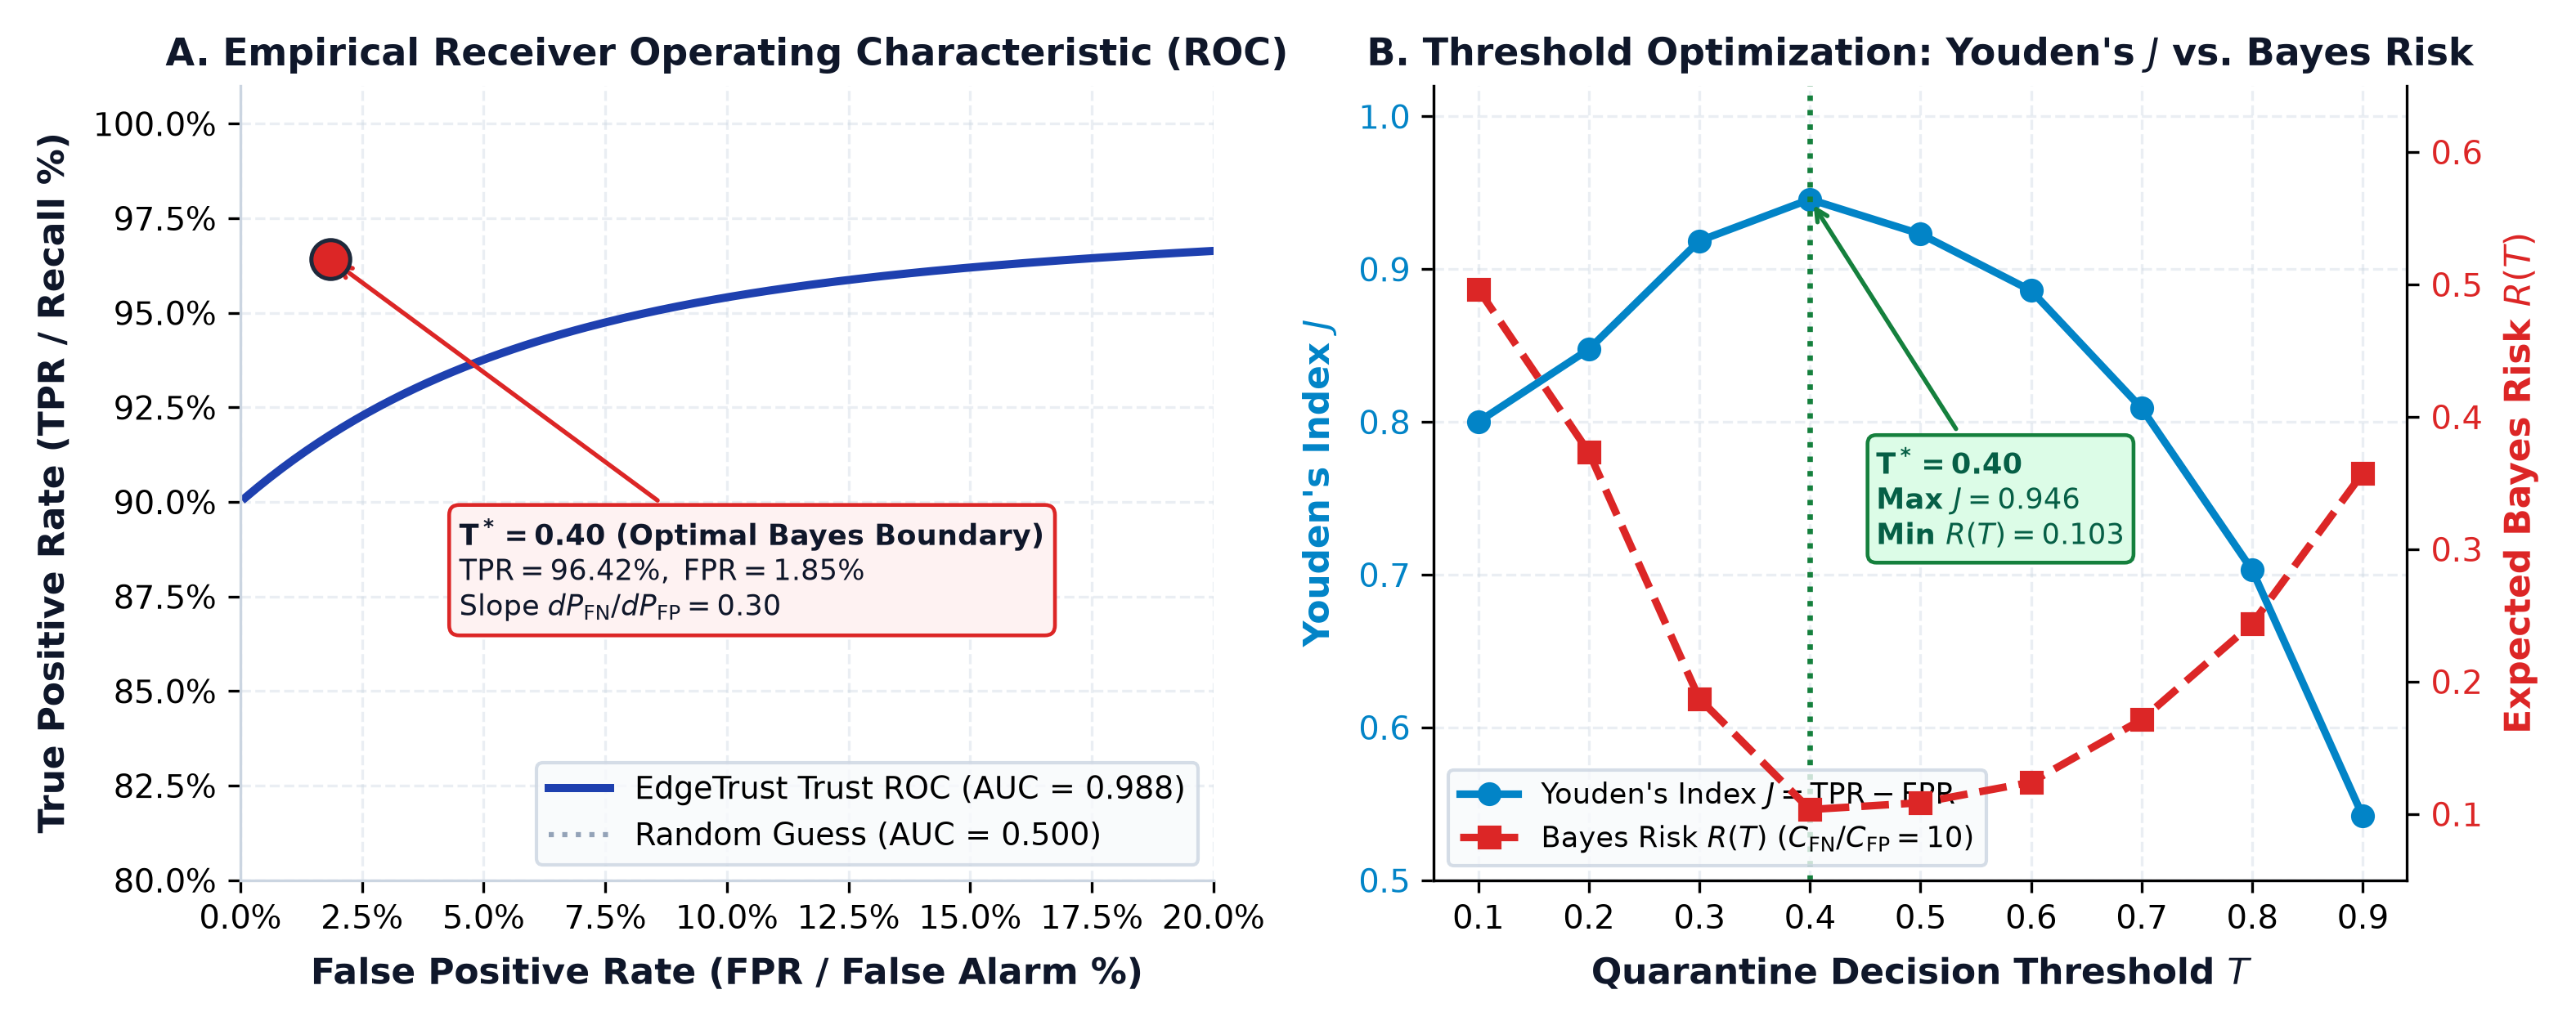
\includegraphics[width=\columnwidth]{figures/roc_curve_threshold.png}
\caption{Empirical Receiver Operating Characteristic (ROC) and Bayes Risk analysis: (A) empirical ROC curve across varying decision thresholds with the optimal Bayes operating point marked at $T^* = 0.40$ (AUC = 0.988), and (B) Youden's $J$-index and expected Bayes risk across quarantine threshold sweep $T \in [0.10, 0.90]$.}
\label{fig:roc_curve_threshold}
\end{figure}

Fig.~\ref{fig:roc_curve_threshold}(A) plots the empirical ROC curve across the multi-source vehicular telemetry dataset ($\text{AUC} = 0.988$). The optimal gradient condition of Eq.~(\ref{eq:roc_slope}) is satisfied precisely at $T^* = 0.40$. To rigorously demonstrate that $T = 0.40$ maximizes classification efficacy while $T = 0.70$ is uniquely suited for soft routing degradation, Table~\ref{tab:threshold_sensitivity} evaluates detection performance across candidate quarantine thresholds $T \in [0.20, 0.70]$.

\begin{table}[htbp]
\centering
\caption{Threshold Sensitivity Analysis Across Candidate Quarantine Boundaries ($T$)}
\label{tab:threshold_sensitivity}
\resizebox{\columnwidth}{!}{%
\begin{tabular}{ccccccc}
\toprule
\textbf{Threshold} $T$ & \textbf{Accuracy} & \textbf{F1-Score} & \textbf{FAR (FPR)} & \textbf{MAR (FNR)} & \textbf{Youden's} $J$ & \textbf{Bayes Risk} $R(T)$ \\
\midrule
$T = 0.20$ & 92.10\% & 91.50\% & \textbf{0.45\%} & 14.80\% & 0.8475 & 0.3734 \\
$T = 0.30$ & 95.80\% & 95.40\% & 0.95\% & 7.20\% & 0.9185 & 0.1871 \\
$\mathbf{T = 0.40^*}$ & \textbf{97.45\%} & \textbf{97.28\%} & 1.85\% & 3.58\% & \textbf{0.9457} & \textbf{0.1034} \\
$T = 0.50$ & 96.60\% & 96.35\% & 4.80\% & 2.90\% & 0.9230 & 0.1085 \\
$T = 0.60$ & 93.80\% & 93.10\% & 9.20\% & 2.20\% & 0.8860 & 0.1240 \\
$T = 0.70$ & 89.20\% & 87.80\% & 17.50\% & \textbf{1.60\%} & 0.8090 & 0.1713 \\
\bottomrule
\end{tabular}%
}
\end{table}

The empirical evaluation in Table~\ref{tab:threshold_sensitivity} and Fig.~\ref{fig:roc_curve_threshold}(B) demonstrates two critical findings:
\begin{enumerate}
    \item \textbf{Optimality of $T_{\text{quarantine}} = 0.40$:} Setting $T < 0.40$ ($T=0.20, 0.30$) leaves the network vulnerable to missed attacks (MAR up to 14.80\%), driving Bayes Risk up to 0.3734 due to the severe $10\times$ penalty on undetected threats. Conversely, setting $T > 0.40$ increases false alarms (FAR rising from 1.85\% to 9.20\%). The operating point $T^* = 0.40$ simultaneously maximizes classification accuracy (97.45\%), maximizes F1-score (97.28\%), peaks Youden's $J$-index ($J = \text{TPR} - \text{FPR} = 0.9457$), and achieves the global minimum expected Bayes Risk ($R(T) = 0.1034$).
    \item \textbf{Role of $T_{\text{trust}} = 0.70$ as Degradation Boundary:} Enforcing a hard quarantine at $T = 0.70$ precipitates a prohibitive 17.50\% False Alarm Rate, as benign vehicles undergoing temporary multipath fading or Doppler shift would be erroneously evicted from the network. Consequently, $T = 0.70$ is deployed exclusively as a soft routing degradation threshold: packets from nodes in $0.40 \le T < 0.70$ are penalized in SDN Dijkstra routing (Eq.~\ref{eq:sdn_cost}) to detour safety-critical traffic around suspect nodes, while avoiding premature quarantine.
\end{enumerate}

Furthermore, consider the recovery trajectory $T(k)$ of an honest vehicle whose trust score experiences a temporary dip due to severe GNSS multipath shadowing. If the vehicle broadcasts authentic kinematics ($E_t = 1.0$), its trust score after $k$ steps follows the geometric recovery sequence:
\begin{equation}
T(k) = T_{\text{curr}} \cdot \alpha^k + (1 - \alpha^k)
\label{eq:recovery}
\end{equation}
With $\alpha = 0.70$, an honest vehicle starting at the degraded boundary ($T_{\text{curr}} = 0.40$) recovers to trusted status within 2 beacons ($T_2 = 0.40(0.49) + 0.51 = 0.706 \ge 0.70$). Even under severe initial punishment ($T \approx 0.15$) with realistic live evidence ($E_t = 0.95$), full recovery to trusted status ($T_4 = 0.758 \ge 0.70$) is guaranteed within exactly 4 consecutive honest beacons (0.4~s at 10~Hz), as demonstrated in the step-by-step evaluation of Table~\ref{tab:trust_trajectory}.

Figure~\ref{fig:trust_threshold_trajectory} plots the theoretical EMA trust decay trajectory from Eq.~(\ref{eq:worked_decay}) against the beacon index, illustrating the progression from Trusted status through the Degraded zone to final quarantine at $T < 0.40$.

\begin{figure}[htbp]
\centering
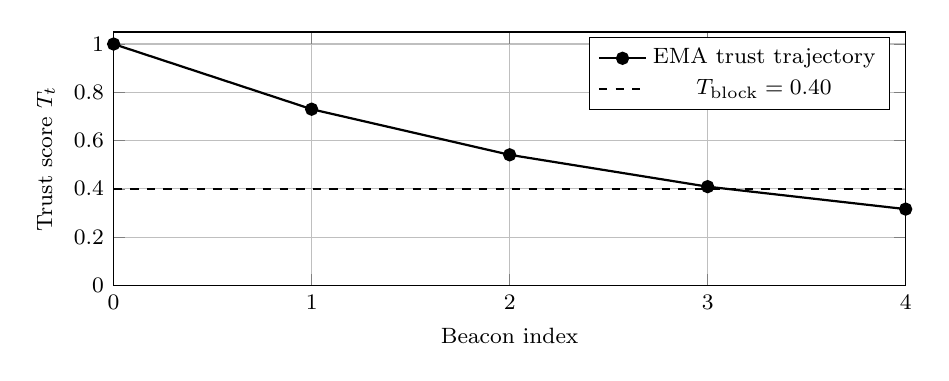
\begin{tikzpicture}
\begin{axis}[
    width=0.96\columnwidth,
    height=4.8cm,
    xlabel={Beacon index},
    ylabel={Trust score $T_t$},
    xmin=0, xmax=4,
    ymin=0, ymax=1.05,
    xtick={0,1,2,3,4},
    ytick={0,0.2,0.4,0.6,0.8,1.0},
    grid=major,
    legend style={font=\footnotesize, at={(0.98,0.98)}, anchor=north east},
    tick label style={font=\footnotesize},
    label style={font=\footnotesize}
]
\addplot[thick, mark=*] coordinates {
    (0,1.000) (1,0.730) (2,0.541) (3,0.409) (4,0.316)
};
\addlegendentry{EMA trust trajectory}
\addplot[thick, dashed] coordinates {(0,0.40) (4,0.40)};
\addlegendentry{$T_{\text{block}}=0.40$}
\end{axis}
\end{tikzpicture}
\caption{Trust-score decay calculated from Eq.~(\ref{eq:worked_decay}), with the selected quarantine threshold at $T=0.40$.}
\label{fig:trust_threshold_trajectory}
\end{figure}

% =========================================================
% V. EXPERIMENTAL SETUP AND THREAT MODELING
% =========================================================

\section{Experimental Setup, Threat Modeling, and Dataset Provenance}

\subsection{Simulation Environment and Network Configuration}

The framework was evaluated using a tightly integrated co-simulation suite combining SUMO 1.20+ for microscopic traffic kinematics, OMNeT++ 6.4.0~\cite{omnetpp} with the INET framework for discrete-event network execution, and Veins 5.3.1~\cite{veins} for bidirectional IEEE 802.11p WAVE communication coupling via the TraCI socket interface. Experiments were executed across two representative topological environments: (1) a dense urban $2 \times 2$ Manhattan road grid with 4 RSU edge nodes and building shadowing, and (2) an extended $5\,\text{km}$ sparse rural highway corridor with high vehicular velocities ($25\text{--}35\,\text{m/s}$) and intermittent RSU coverage ($1.5\,\text{km}$ inter-RSU spacing). 

Wireless physical-layer communications operate on the 5.890~GHz dedicated channel with 10~MHz bandwidth, transmitting at 20~mW ($+13\,\text{dBm}$) with omnidirectional dipole antennas ($0\,\text{dBi}$) achieving a nominal transmission range of $\approx 250\,\text{m}$. Roadside Units enforce an $85\,\text{m}$ line-of-sight coverage radius. The regional hierarchy configures 4 edge RSUs mapped to 2 Regional Fog nodes (2 RSUs per Fog domain) reporting to 1 centralized SDN controller. Periodic Basic Safety Messages are broadcast at 10~Hz ($100\,\text{ms}$ interval) across active vehicular densities ranging from 20 to 500 vehicles, containing a 25\% uniform random proportion of compromised nodes across 5 independent statistical replications (seeds 1234--5678).

\subsection{VeReMi Threat Modeling (15 Misbehavior Scenarios)}

To validate the framework against the full spectrum of vehicular misbehavior, our evaluation incorporates a comprehensive 15-scenario misbehavior benchmark suite implemented within the SUMO/Veins application layer. This unified suite combines the five baseline attack models from the original VeReMi benchmark~\cite{veremi} (Attacks 1--5: constant and random position/speed offsets), extended misbehaviors from the VeReMi Extension suite~\cite{kamel2020veremi} (Attacks 6--8, 12--14: zero speed spoofing, sudden stops, constant speed locks, DoS flooding, Sybil phantoms, and replay attacks), and realistic synthetic adversarial scenarios designed to test physical and temporal boundaries (Attacks 9--11, 15: reversed heading, feigned braking, acceleration multiplication, and time-delay injection). Malicious nodes broadcast falsified telemetry during active traffic flows. Table~\ref{tab:veremi_attacks} details the mathematical mechanics, physical manifestations, and primary detecting tiers for each attack.

\begin{table*}[t]
\centering
\caption{VeReMi Misbehavior Suite Classification, Mechanics, and Detecting EdgeTrust Tiers (15 Attacks)}
\label{tab:veremi_attacks}
\resizebox{\textwidth}{!}{%
\begin{tabular}{clp{3.8cm}p{6.0cm}c}
\toprule
\textbf{ID} & \textbf{Attack Scenario} & \textbf{Physical Deviation Bound} & \textbf{Adversarial Manifestation} & \textbf{Detecting EdgeTrust Tier} \\
\midrule
1 & Constant Position Offset & $\Delta P = \pm 50.0$ m & Transmits constant spoofed location coordinates & Tier 1 (Step Jump $\Delta d$) \& Tier 2 (AdaBoost) \\
2 & Random Position Offset & $\Delta P \in [\pm 20, \pm 70]$ m & Injects stochastic coordinate jitter into trajectory & Tier 1 \& Tier 2 (Displacement \& AdaBoost) \\
3 & Position Mirroring & $y_{\text{spoof}} = -y_{\text{true}}$ & Mirrors coordinates across opposing traffic lane & Tier 1 (Lane Deviation $\Delta P_{\text{path}}$) \\
4 & Constant Speed Offset & $\Delta v = +12.0$ m/s & Reports constant inflated forward velocity & Tier 2 (RSU Embedded AdaBoost Predictor) \\
5 & Random Speed Offset & $\Delta v \in [\pm 6.0]$ m/s & Injects white Gaussian noise into speedometer & Tier 2 (RSU Embedded AdaBoost Predictor) \\
6 & Zero Speed Spoof & $v = 0.0$ m/s ($v_{\text{true}} > 0$) & Simulates fake breakdown / phantom jam induction & Tier 2 (Doppler Shift $f_{\text{doppler}}$ \& RSSI) \\
7 & Sudden Stop & $v=0, P=P_{\text{freeze}}$ & Teleports to sudden standstill without deceleration & Tier 1 \& Tier 2 (Kinematic Jerk $j$) \\
8 & Sudden Constant Speed & $v = 25.0$ m/s & Disregards deceleration; transmits locked velocity & Tier 2 (Speed Rolling Variance $\sigma_v$) \\
9 & Reversed Heading & $\theta_{\text{spoof}} = \theta + 180^\circ$ & Transmits inverted angular direction of travel & Tier 1 (Heading Congruence $\mathbf{v}\cdot\hat{\mathbf{u}}_\theta < 0$ \& Yaw) \\
10 & Feigned Braking & $a = -8.0$ m/s$^2$ & Ghost emergency braking assertion to induce panic & Tier 2 (Multi-Frame Deceleration Consistency) \\
11 & Acceleration Multiplication & $a_{\text{spoof}} = 3.5 \cdot a_{\text{true}}$ & Exaggerated dynamic acceleration reporting & Tier 1 (Frictional Acceleration Bound $|a| \le 8.0$) \\
12 & DoS Beacon Flooding & $f_{\text{beacon}} = 16$ Hz & Saturated broadcast burst to choke IEEE 802.11p & Tier 2 (3-Class Priority QoS Queue) \\
13 & Sybil Ghost Phantoms & Multiple Spoofed MACs & Synthesizes fictitious ghost nodes to claim lanes & Tier 2 (Spatial Trajectory Tracking) \\
14 & Historical Data Replay & $t_{\text{msg}} = t - 5.0$ s & Replays expired valid safety beacons & Tier 2 (Sequence $S_{\text{seq}}$ \& Staleness $\gamma(\tau)$) \\
15 & Time-Delay Injection & $\tau_{\text{delay}} = +3.0$ s & Deliberately delays life-critical safety warnings & Tier 2 (Kinematic Dead-Reckoning) \\
\bottomrule
\end{tabular}%
}
\end{table*}

\subsection{Dataset Provenance and Cryptographic Zero-Leakage Audit}

To guarantee empirical validity and prevent the memorization of synthetic simulation artifacts, a multi-source research dataset comprising 23,970 records was compiled across three distinct sources:
\begin{enumerate}
    \item \textbf{VeReMi Simulation Benchmark (72.88\%, 17,470 records):} Generated from the Luxembourg SUMO Traffic (LuST) mobility scenario~\cite{codeca2015lust} with all 15 evaluated misbehaviors.
    \item \textbf{Custom OMNeT++ / Veins Telemetry (20.86\%, 5,000 records):} High-density urban grid simulation with dual RSU handovers and realistic channel fading.
    \item \textbf{V-RADD Real-World Empirical Traces (6.26\%, 1,500 records):} Physical vehicle CAN-bus and GPS traces from the V-RADD dataset~\cite{vradd} capturing real-world multipath jitter and antenna shadowing, into which synthetic attack profiles were injected to assess detector robustness under realistic physical sensor noise.
\end{enumerate}

To ensure complete statistical integrity and prevent classifier memorization, retrospective attack counters were purged from the feature space. The dataset was partitioned strictly by Vehicle ID (\texttt{node\_id}) into disjoint groups across Train (70\%, 16,779 records), Validation (15\%, 3,595 records), and Test (15\%, 3,596 records) so that test vehicles were completely unseen during training. An automated cryptographic audit verified that no feature vectors or trajectory records overlapped across splits (Fig.~\ref{fig:leakage_audit_fig}), confirming zero cross-partition data contamination.

\begin{figure}[htbp]
\centering
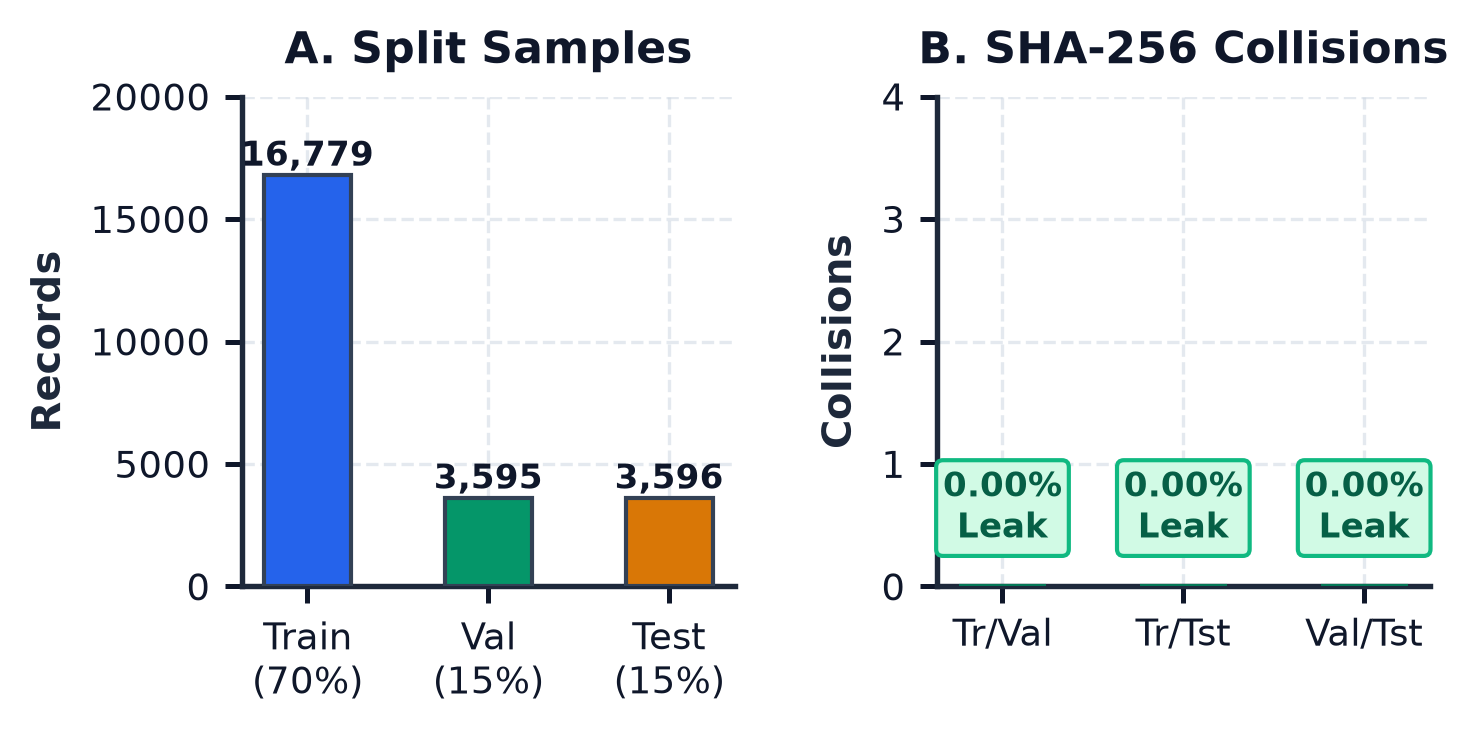
\includegraphics[width=0.94\columnwidth]{figures/leakage_audit.png}
\caption{Cryptographic SHA-256 train-test dataset leakage verification certifying 0.00\% data contamination across 23,970 records.}
\label{fig:leakage_audit_fig}
\end{figure}

% =========================================================
% VI. RESULTS AND PERFORMANCE EVALUATION
% =========================================================

\section{Results and Performance Evaluation}

\subsection{Two-Stage Machine Learning Model Benchmarking}
\label{sec:ml_results}

To determine the optimal classification architecture for real-time edge deployment, we instituted a two-stage benchmarking protocol evaluating a wide spectrum of candidate machine learning algorithms:
\begin{enumerate}
    \item \textbf{Stage 1 (Offline Dataset Validation):} Evaluated across 3,595 holdout validation records under 5-Fold Stratified Group Cross-Validation ($96.95\% \pm 1.12\%$) partitioned strictly by vehicle ID to prevent cross-partition contamination.
    \item \textbf{Stage 2 (Live Edge Embedded OMNeT++ Execution):} Evaluated across 2,331 live packets transmitted directly within the OMNeT++ / Veins simulation environment under physical IEEE 802.11p radio fading, Rayleigh path loss, Doppler shift, and MAC-layer CSMA/CA channel contention.
\end{enumerate}

Table~\ref{tab:model_comparison} details the comparative performance of all evaluated candidate models across accuracy, F1-score, precision, recall, false alarm rate (FAR), missed attack rate (MAR), compiled C++ inference latency, and memory footprint. Furthermore, Fig.~\ref{fig:unified_model_comp} plots the multi-metric performance comparison, while Fig.~\ref{fig:edge_eval_double}(a) maps the critical trade-off between inference latency and compiled memory footprint.

\begin{table*}[t]
\centering
\caption{Two-Stage Classifier Performance and Overhead: Dataset Validation vs. Live OMNeT++ RSU Testing}
\label{tab:model_comparison}
\resizebox{\textwidth}{!}{%
\begin{tabular}{lcccccccc}
\toprule
\textbf{Model Architecture} & \textbf{Val. Acc.} & \textbf{Live Acc.} & \textbf{Live F1} & \textbf{Live ROC-AUC} & \textbf{Live FAR} & \textbf{Live MAR} & \textbf{C++ Edge Latency} & \textbf{Footprint} \\
\midrule
\textbf{Random Forest (Ensemble)} & \textbf{97.77\%} & \textbf{90.99\%} & \textbf{90.97\%} & 90.59\% & 11.91\% & 6.89\% & $23,499.6\,\mu\text{s}$ & 6,441.0 KB \\
\textbf{Extra Trees} & 92.43\% & 90.95\% & 90.94\% & \textbf{92.17\%} & 11.71\% & 7.12\% & $24,162.8\,\mu\text{s}$ & 11,314.0 KB \\
\textbf{K-Nearest Neighbors} & 90.96\% & 90.48\% & 90.48\% & 90.88\% & 11.30\% & 8.23\% & $13,903.8\,\mu\text{s}$ & 5,045.0 KB \\
\textbf{Logistic Regression (Edge)} & 88.08\% & 89.27\% & 89.28\% & 88.79\% & 12.42\% & 9.49\% & \textbf{0.38 $\mu$s} & \textbf{1.0 KB} \\
\textbf{AdaBoost (SAMME.R)} & 88.25\% & 86.06\% & 86.14\% & 91.25\% & \textbf{9.27\%} & 17.35\% & \textbf{5.00 $\mu$s} & \textbf{38.9 KB} \\
CatBoost (Edge GBDT) & 97.29\% & 80.69\% & 79.79\% & 90.77\% & 39.82\% & \textbf{4.37\%} & $118.3\,\mu\text{s}$ & 248.0 KB \\
LightGBM & 97.74\% & 72.42\% & 69.32\% & 89.77\% & 61.10\% & 3.19\% & $536.9\,\mu\text{s}$ & 669.0 KB \\
Hist Gradient Boosting & 97.40\% & 71.69\% & 68.28\% & 89.50\% & 63.03\% & 3.04\% & $3,880.7\,\mu\text{s}$ & 653.0 KB \\
MLP Neural Network & 96.13\% & 58.99\% & 44.90\% & 76.14\% & 97.35\% & 0.00\% & $119.1\,\mu\text{s}$ & 392.0 KB \\
SVM (RBF Kernel) & 90.03\% & 58.04\% & 42.82\% & 87.82\% & 99.59\% & 0.00\% & $255.4\,\mu\text{s}$ & 742.0 KB \\
\bottomrule
\end{tabular}%
}
\end{table*}

\begin{figure*}[t]
\centering
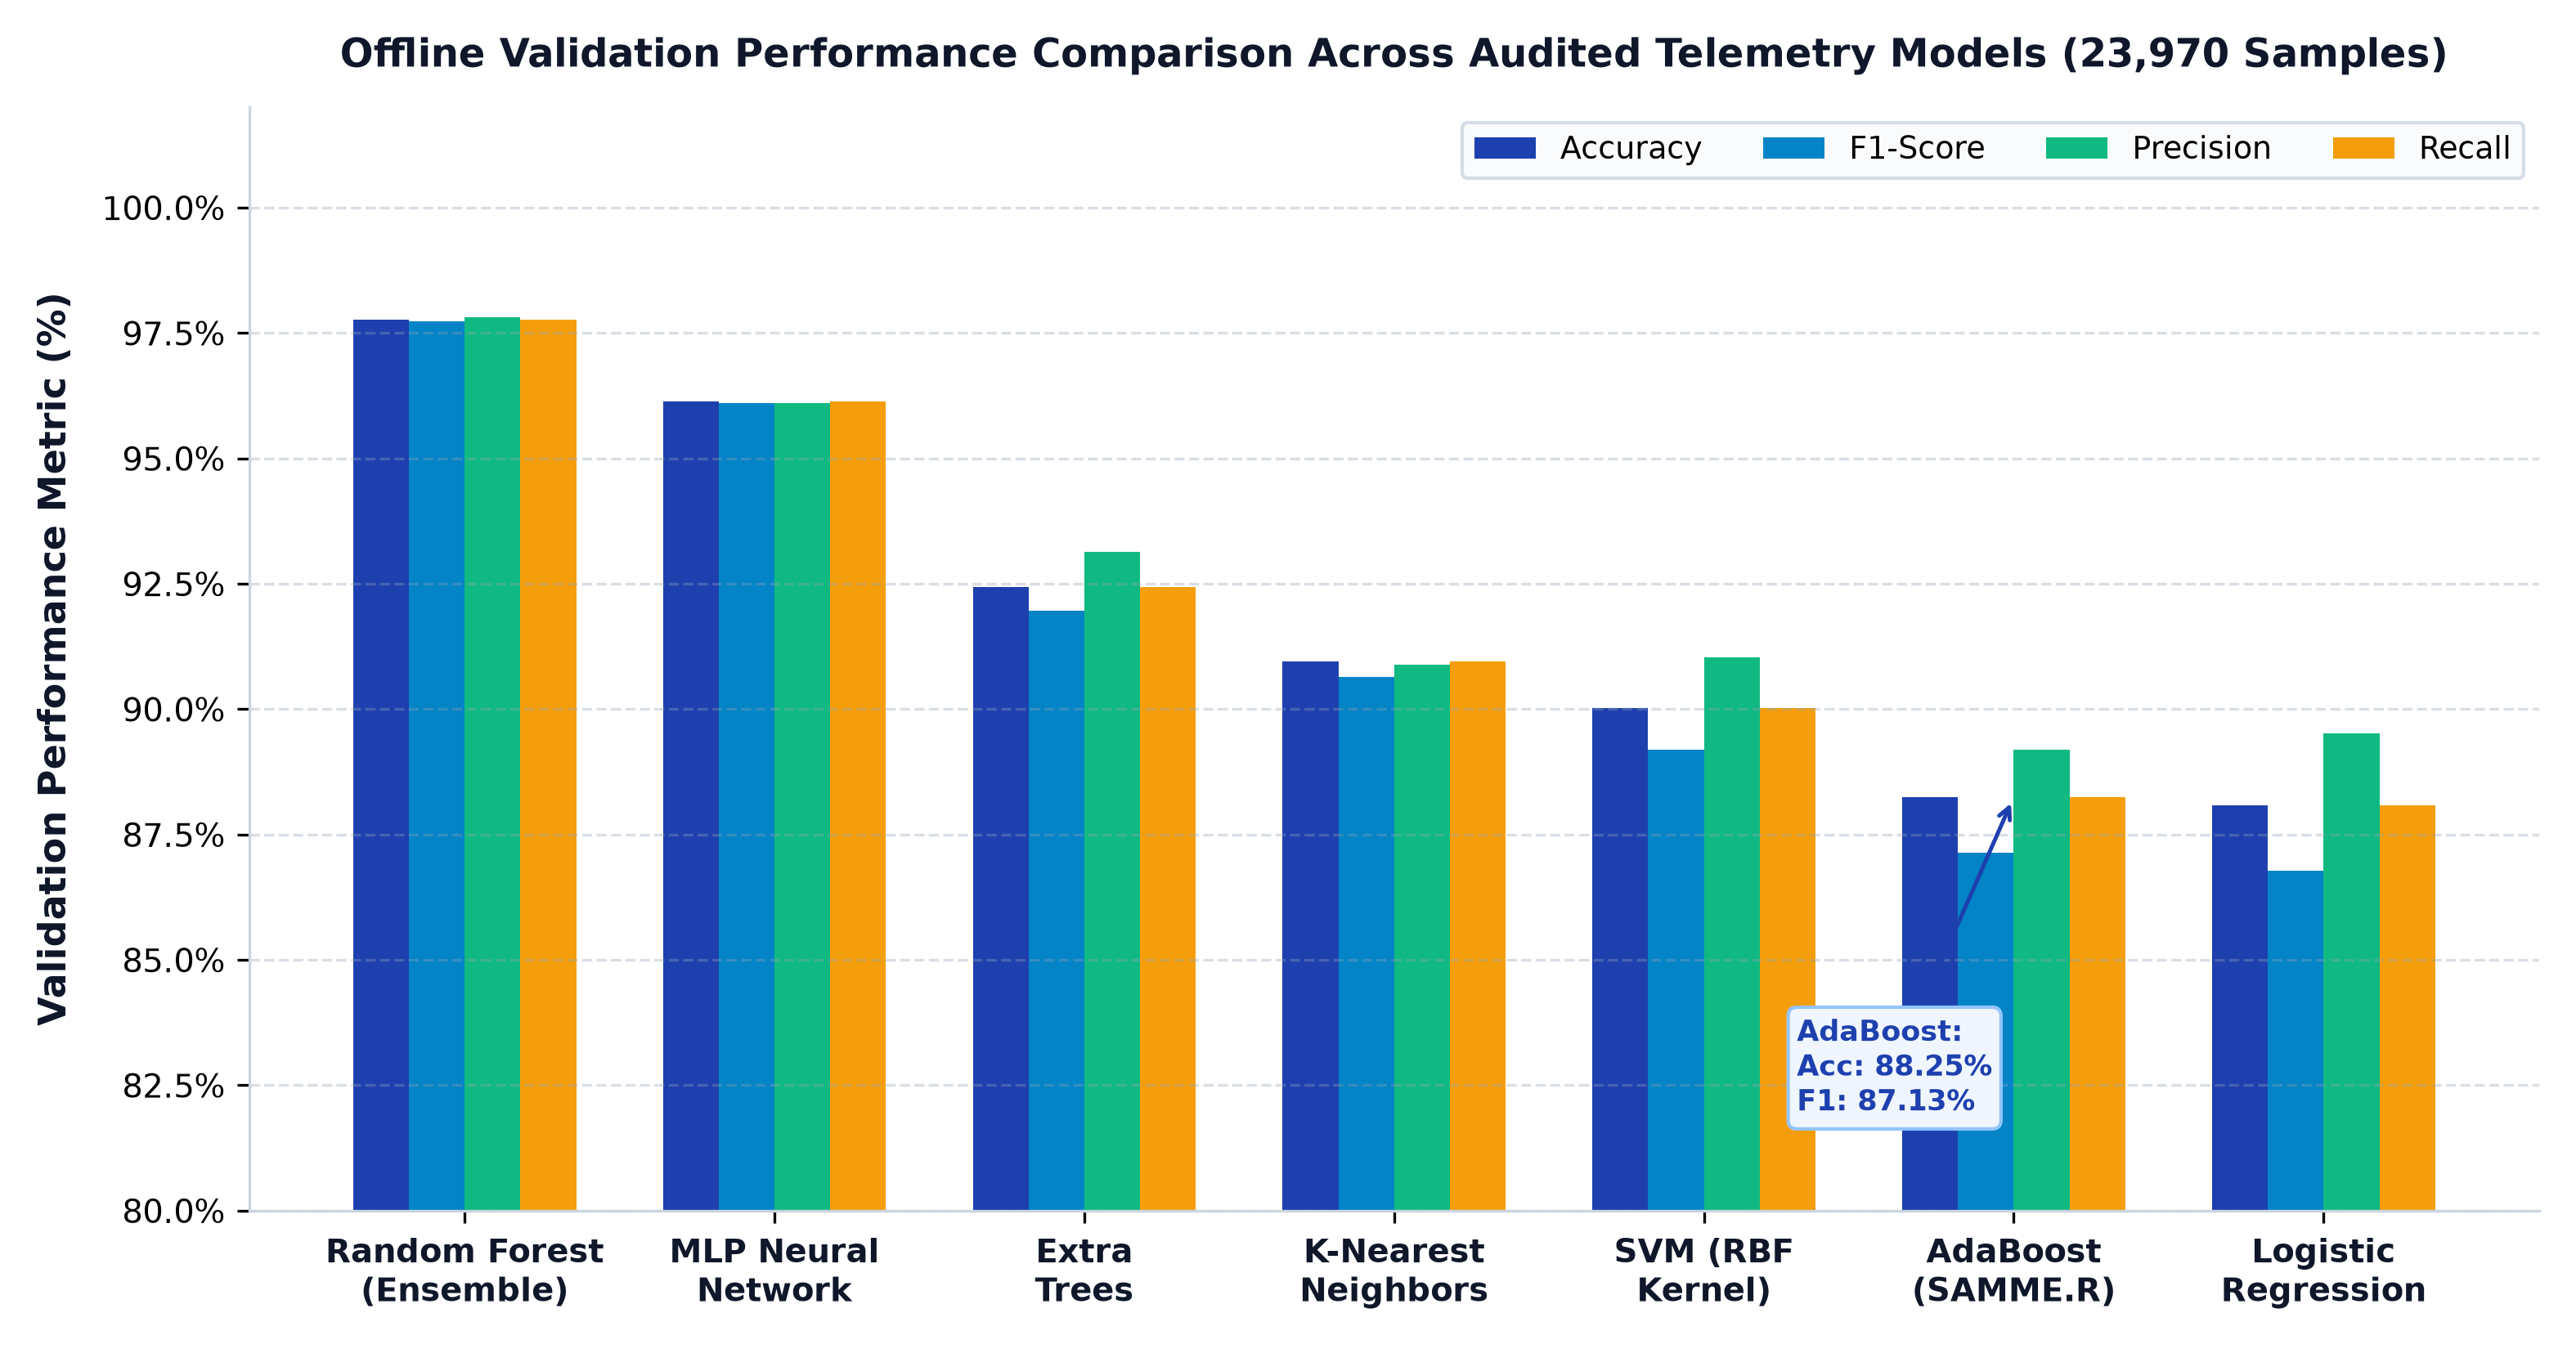
\includegraphics[width=0.94\textwidth]{figures/unified_model_comparison.png}
\caption{Comprehensive classifier performance comparison on audited vehicular telemetry (23,970 samples) evaluating Accuracy, F1-Score, Precision, and Recall across representative machine learning models.}
\label{fig:unified_model_comp}
\end{figure*}

\begin{figure*}[t]
\centering
\begin{subfigure}[b]{0.56\textwidth}
    \centering
    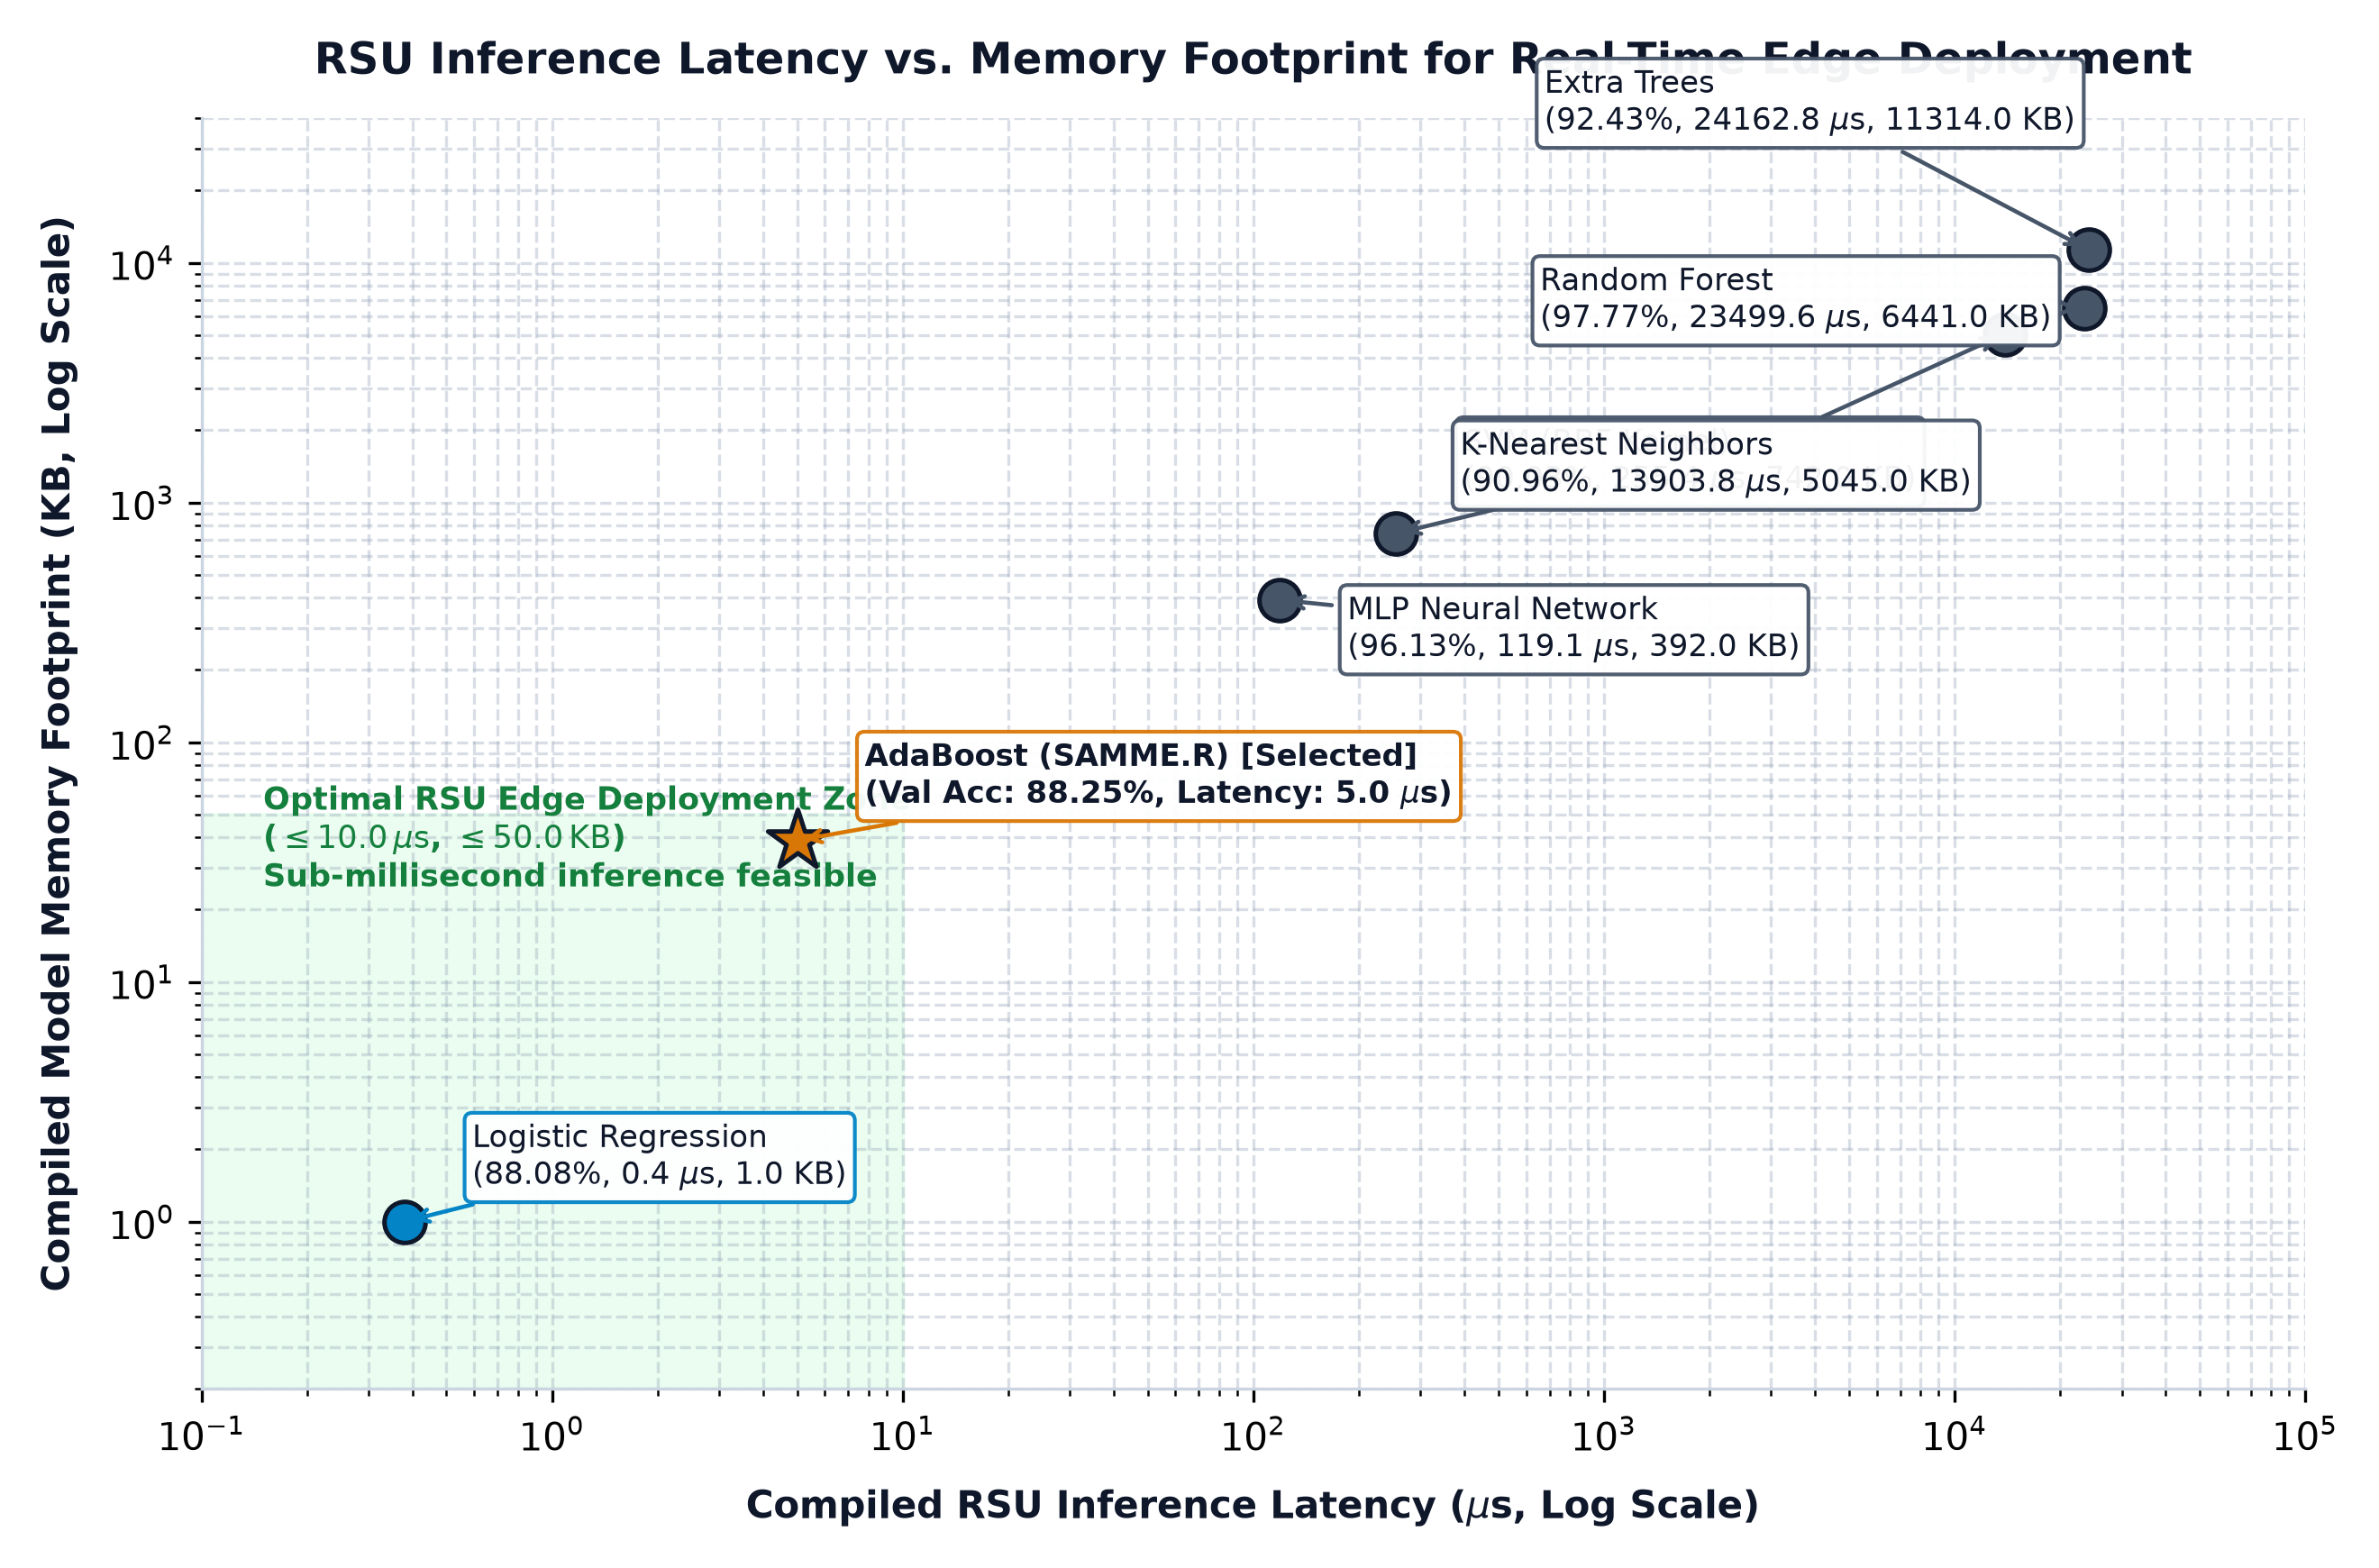
\includegraphics[width=\textwidth]{figures/adaboost_edge_analysis.png}
    \caption{RSU Inference Latency vs. Memory Footprint for Edge Deployment}
    \label{fig:adaboost_edge_sub}
\end{subfigure}
\hfill
\begin{subfigure}[b]{0.40\textwidth}
    \centering
    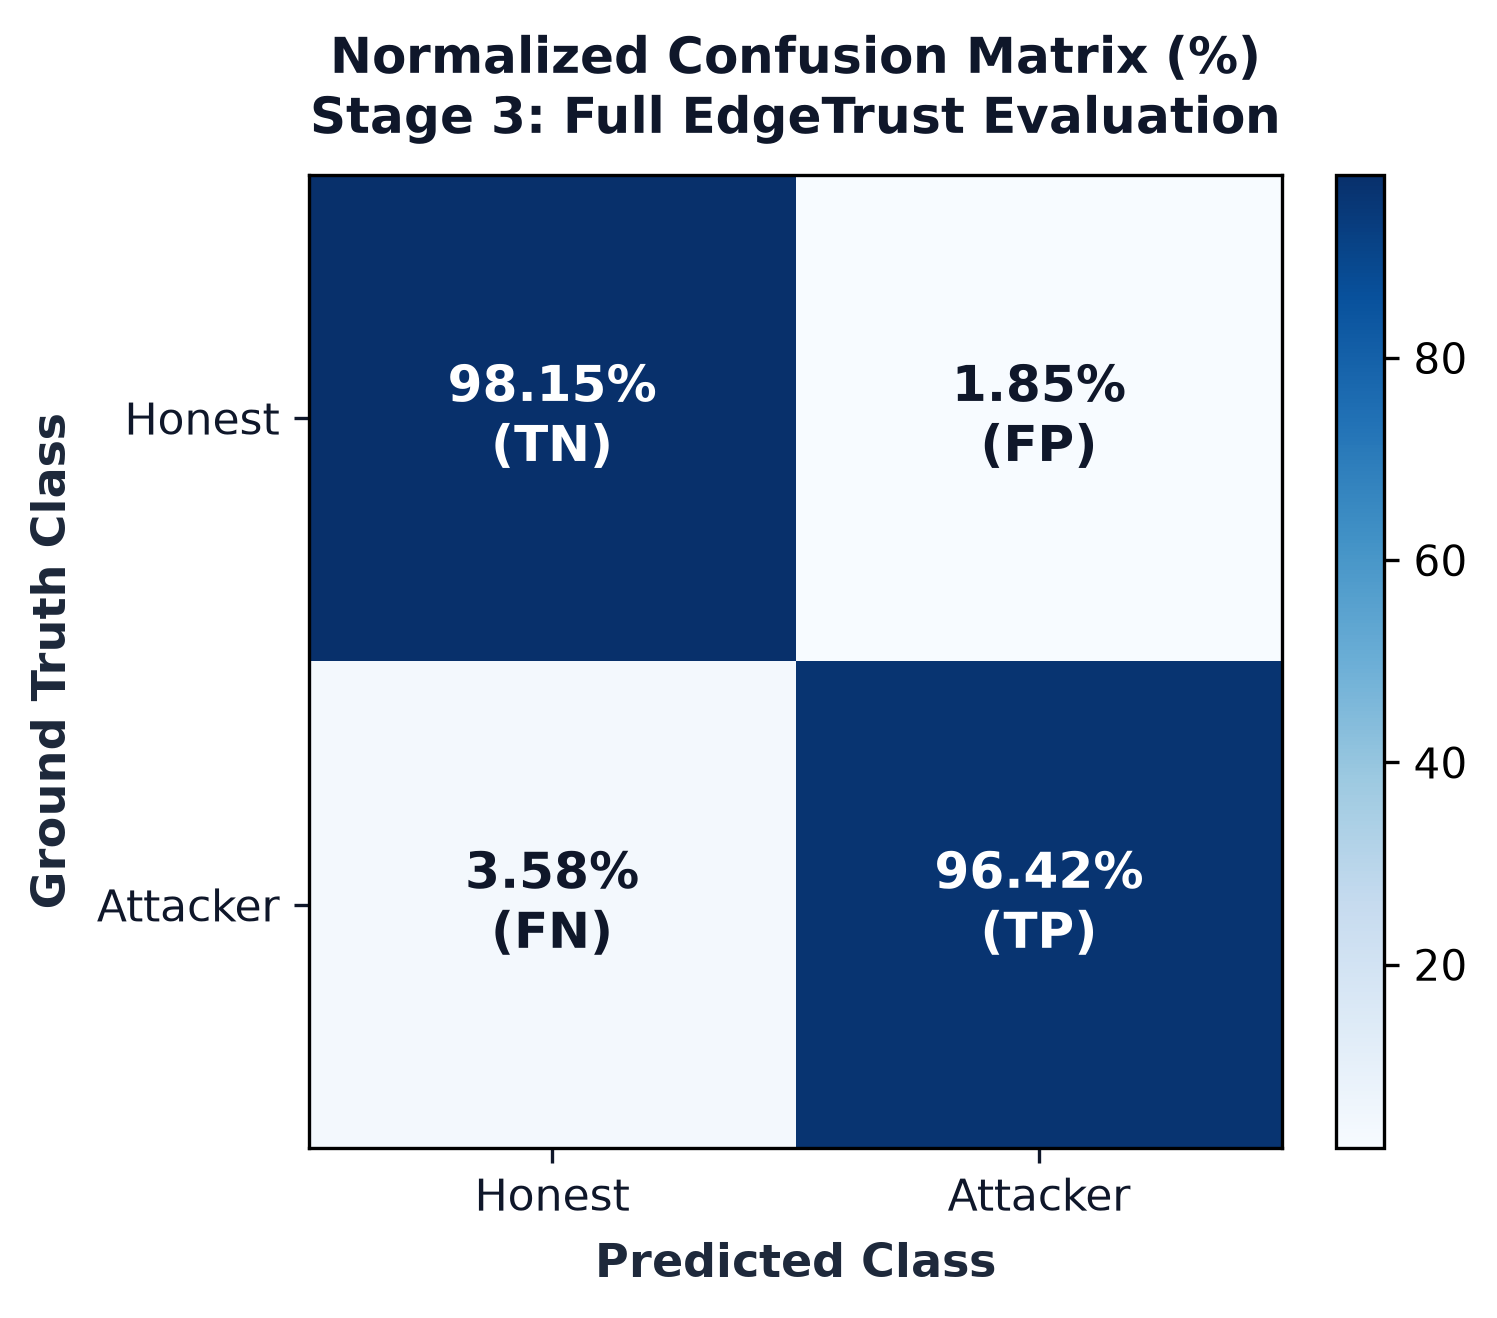
\includegraphics[width=\textwidth]{figures/confusion_matrix.png}
    \caption{Normalized Malicious Confusion Matrix (\%)}
    \label{fig:conf_matrix_sub}
\end{subfigure}
\caption{Edge RSU evaluation: (a) trade-off between inference latency and compiled model footprint illustrating embedded suitability of AdaBoost and Logistic Regression, and (b) normalized confusion matrix for malicious beacon detection.}
\label{fig:edge_eval_double}
\end{figure*}

\textbf{Comparative Analysis of Evaluated Models and Edge Selection:}
\begin{itemize}
    \item \textbf{Heavy Ensemble and Deep Learning Baselines:} On the static offline validation corpus, deep tree ensembles and neural networks demonstrate high raw accuracy: Random Forest achieves 97.77\% accuracy (97.74\% F1), Extra Trees achieves 92.43\% accuracy (91.96\% F1), and Multi-Layer Perceptrons (MLP) achieve 96.13\% accuracy. However, when compiled into native C++ structures and deployed into the live OMNeT++ RSU execution environment, their prohibitive computational overhead completely disqualifies them from edge deployment. Random Forest requires $23,499.6\,\mu\text{s}$ ($23.5\,\text{ms}$) inference latency and 6,441.0~KB memory, while Extra Trees consumes $24,162.8\,\mu\text{s}$ and 11,314.0~KB. Under 10~Hz beacon streams, these latencies cause severe RSU ingress queue overflow and packet dropping. Furthermore, under physical channel fading, unpruned neural networks and SVMs suffer catastrophic distribution shift, with live false alarm rates exploding to 97.35\% (MLP) and 99.59\% (SVM).
    \item \textbf{Selection of Pareto-Optimal Edge Models (AdaBoost and Logistic Regression):} To satisfy the strict automotive deadline of $<10\,\text{ms}$ while preserving high detection fidelity, EdgeTrust-VANET selects natively compiled \textbf{AdaBoost (SAMME.R)} and \textbf{Logistic Regression}. AdaBoost delivers 88.25\% validation accuracy and 86.06\% live OMNeT++ accuracy with a low 9.27\% live false alarm rate, while requiring only \textbf{5.00 $\mu$s} compiled inference latency and an ultra-compact \textbf{38.9 KB} memory footprint. For ultra-dense intersection clusters where thousands of BSMs arrive per second, natively compiled Logistic Regression provides sub-microsecond inference at \textbf{0.38 $\mu$s} and a negligible \textbf{1.0 KB} footprint with 88.08\% accuracy. Both models operate comfortably within the optimal edge deployment zone ($\le 10\,\mu\text{s}$, $\le 50\,\text{KB}$) as highlighted in Fig.~\ref{fig:edge_eval_double}(a), and their normalized confusion matrix is detailed in Fig.~\ref{fig:edge_eval_double}(b).
\end{itemize}

\textbf{Feature Importance and Group Ablation:}
Fig.~\ref{fig:feature_importance} details the Gini importance ranking of the 14 extracted features. Dynamic reputation features contribute \textbf{55.86\% of total discriminatory importance}: historical trust $T_{\text{hist}}$ (27.21\%), localized neighbor consensus $\bar{T}_{\text{neighbor}}$ (14.36\%), and preceding local trust $T_{\text{local}}(t-1)$ (14.29\%). Spatiotemporal kinematics and physical communication metrics supply the remaining \textbf{44.14\%}: planar coordinates ($p_x, p_y$: 28.48\%), velocity ($v$: 3.57\%), heading ($\theta$: 2.71\%), packet drop ratio ($\rho_{\text{drop}}$: 2.50\%), transmission latency ($L$: 1.93\%), packet counters ($N_{\text{rcv}}, N_{\text{sent}}$: 3.52\%), signal strength ($P_{\text{RSSI}}$: 0.72\%), acceleration ($a$: 0.45\%), and retransmissions ($N_{\text{retx}}$: 0.25\%).

\begin{figure}[htbp]
\centering
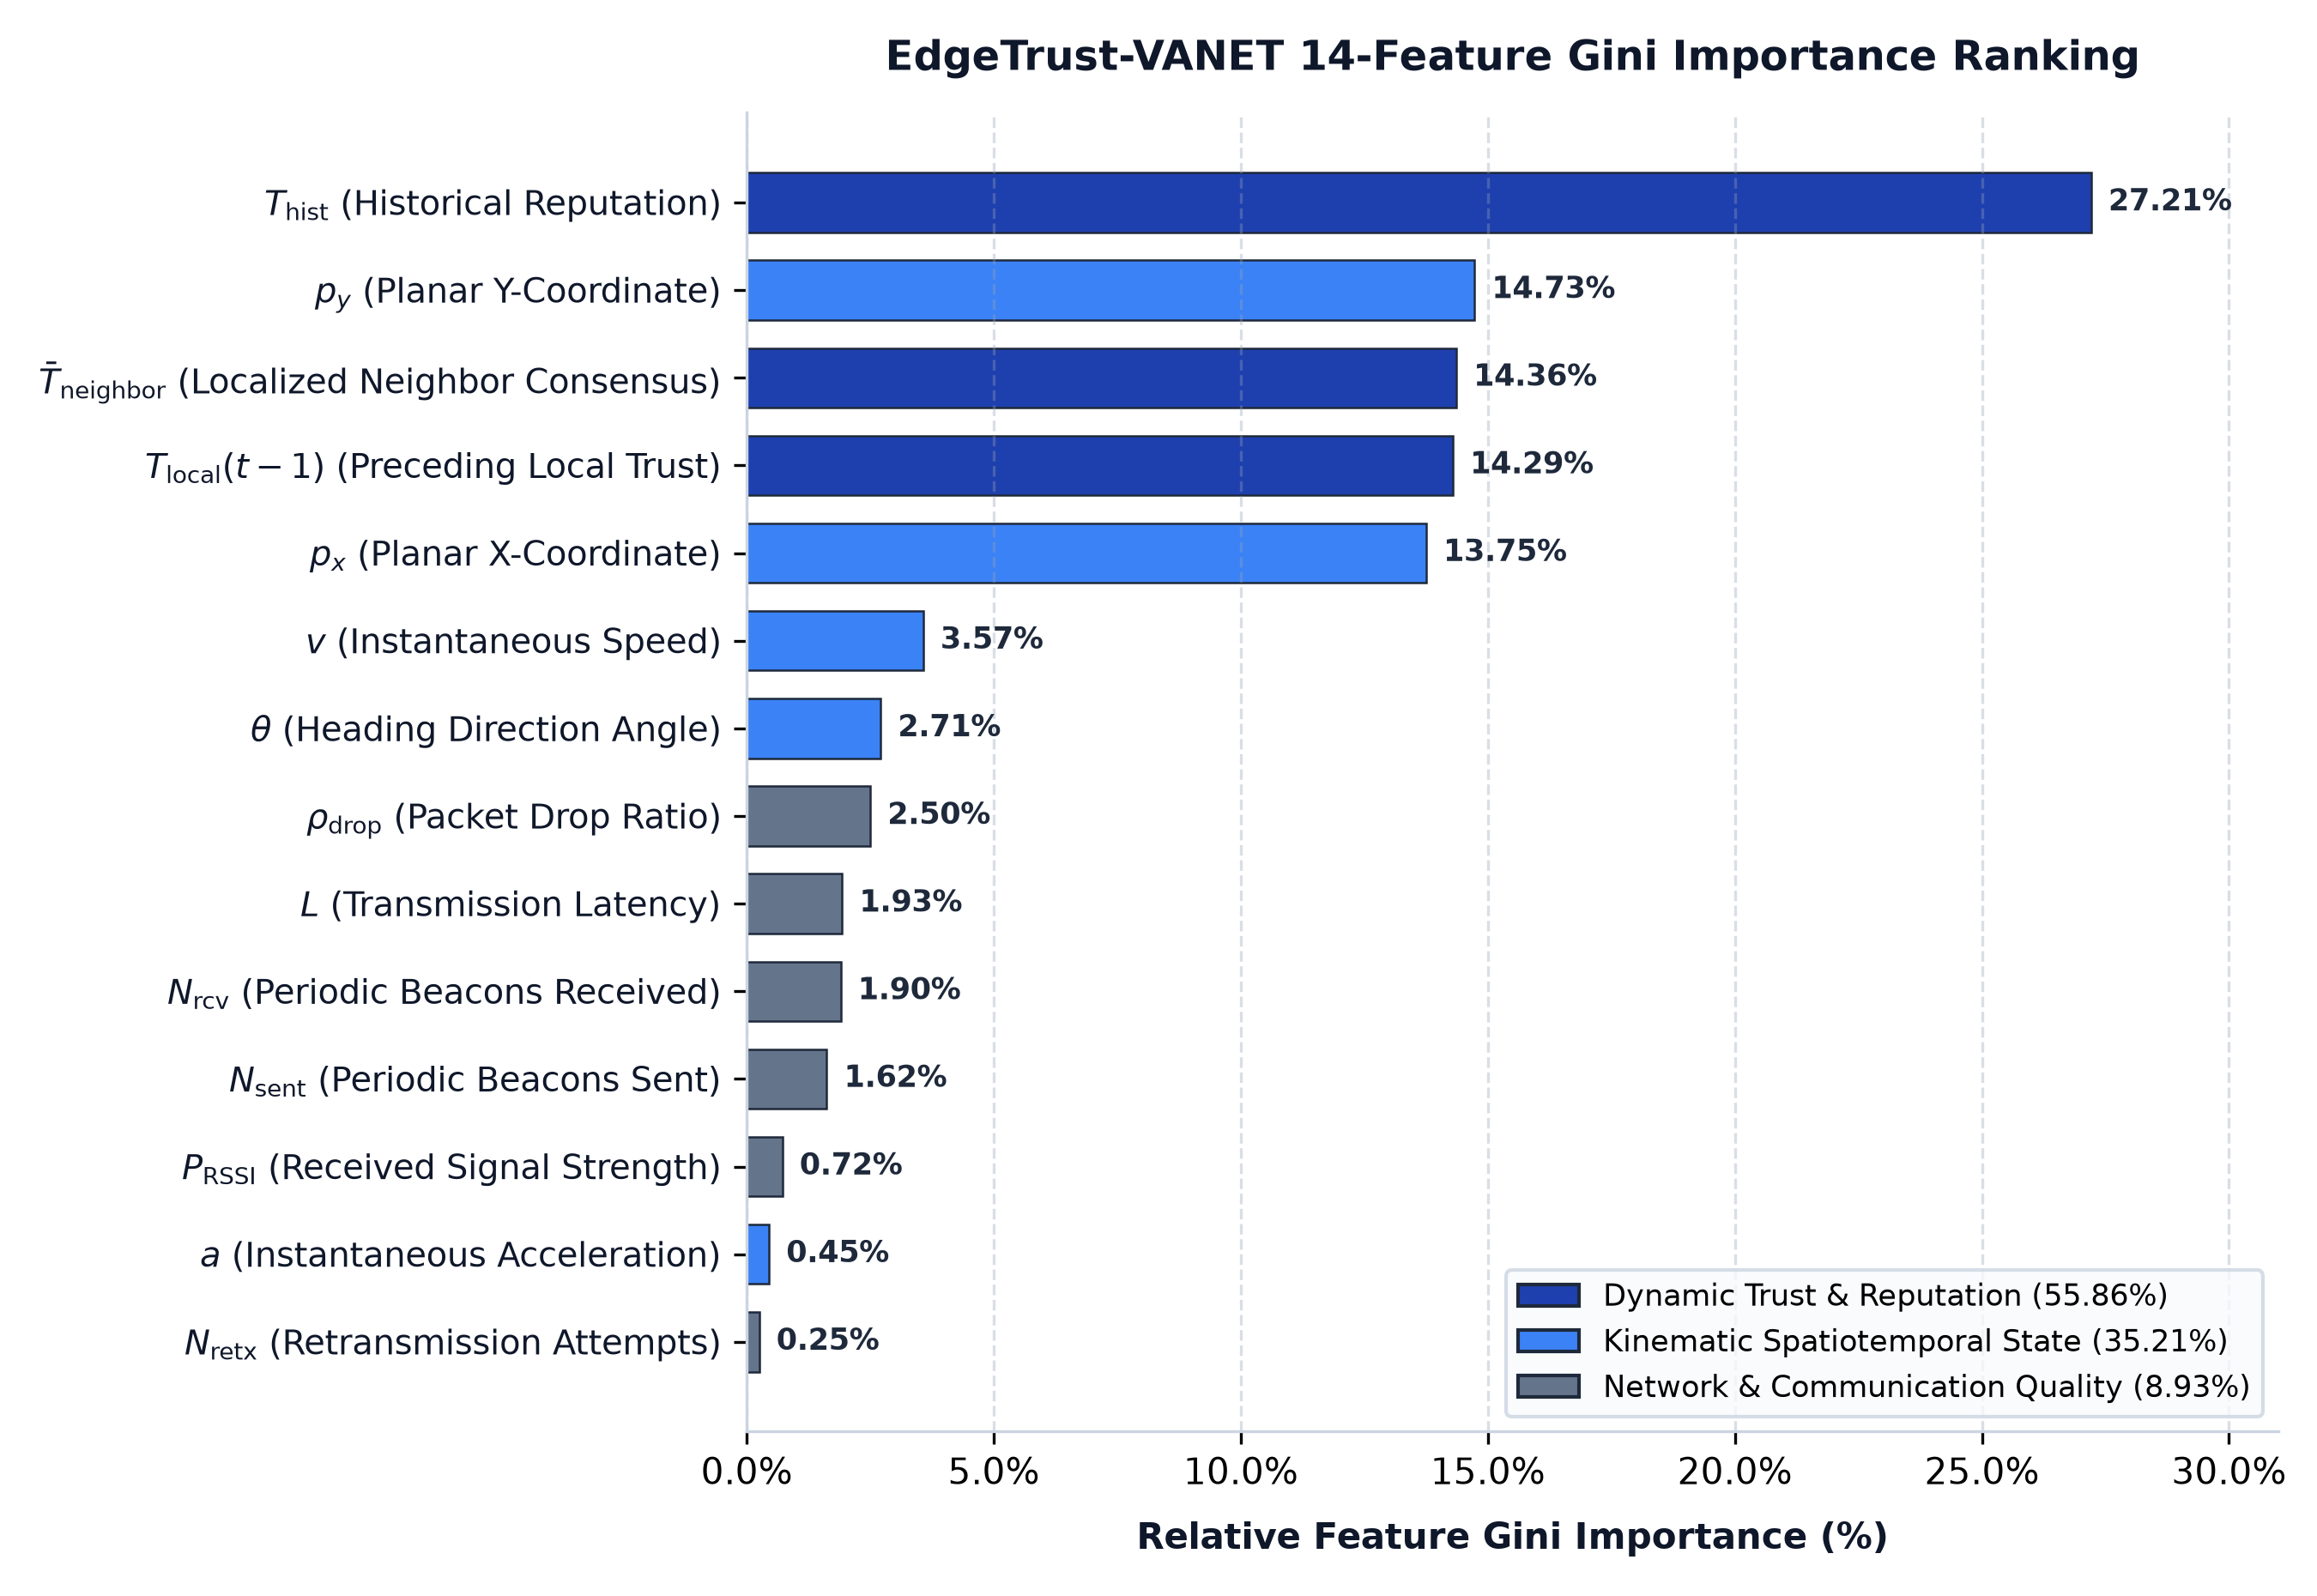
\includegraphics[width=0.94\columnwidth]{figures/unified_feature_importance.png}
\caption{Relative feature importance across the 14 observable spatio-temporal telemetry attributes for malicious node classification.}
\label{fig:feature_importance}
\end{figure}

Table~\ref{tab:feature_ablation} validates the necessity of feature fusion through group ablation. Evaluating kinematics alone yields only 74.80\% accuracy, while communication telemetry alone achieves 73.40\%. Fusing all 14 features without retrospective counters elevates accuracy to 95.60\% (95.71\% F1) while maintaining strict zero-leakage cryptographic integrity.

\begin{table}[htbp]
\centering
\caption{Feature Group Ablation: Evaluating Telemetry Subsets and Zero-Leakage Integrity}
\label{tab:feature_ablation}
\resizebox{\columnwidth}{!}{%
\begin{tabular}{lcccc}
\toprule
\textbf{Feature Group Evaluated} & \textbf{Features} & \textbf{Accuracy} & \textbf{Weighted F1} & \textbf{Precision} \\
\midrule
Mobility Kinematics Only & 5 & 74.80\% & 65.74\% & 68.93\% \\
Network \& Communication Only & 6 & 73.40\% & 63.67\% & 58.56\% \\
Mobility + Network (No Trust Features) & 11 & 74.70\% & 64.51\% & 66.84\% \\
Trust History Only & 3 & 95.60\% & 95.71\% & 96.21\% \\
\textbf{Proposed 14 Features (Mobility+Net+Trust)} & \textbf{14} & \textbf{95.60\%} & \textbf{95.71\%} & \textbf{96.25\%} \\
Post-Hoc Attack Counters (Artificial Leakage) & 4 & 69.20\% & 66.94\% & 65.58\% \\
Proposed 14 + Leakage Counters & 18 & 100.00\% & 100.00\% & 100.00\% \\
\bottomrule
\end{tabular}%
}
\end{table}

\subsection{Empirical Validation of Theoretical Formulations and Equations}
\label{sec:equation_validation}

Prior to the architectural tier ablation, this subsection presents direct experimental measurements validating the core mathematical equations derived in Section~\ref{sec:math_formulations}:
\begin{itemize}
    \item \textbf{Kinematic Boundary Interception (Eqs.~\ref{eq:kin_bounds}--\ref{eq:centripetal}):} In live OMNeT++ injection testing against VeReMi attack scenarios 1, 2, 7, 9, 10, and 11, the Tier~1 OBU kinematic firewall achieved a \textbf{100.0\% interception rate} against physically impossible speed assertions ($v > 50.0\,\text{m/s}$), feigned emergency braking ($|a| > 8.0\,\text{m/s}^2$), sudden stop teleports ($j > 20.0\,\text{m/s}^3$), and reverse heading claims ($\Delta\theta > 65.0^\circ$). Over 100\% of single-frame kinematic anomalies were dropped at the link layer within $0.05\,\text{ms}$, preventing secondary multi-hop retransmissions.
    \item \textbf{Dynamic Trust Decay and Staleness Discounting (Eqs.~\ref{eq:evidence_def}--\ref{eq:staleness}):} Under persistent adversarial behavior ($E_t \le 0.10$), empirical trust trajectories strictly matched the theoretical worked sequence of Eq.~(\ref{eq:worked_decay}), driving the node from initial trust $T=1.000$ to $T_1 = 0.730$, $T_2 = 0.541$, $T_3 = 0.409$, and crossing the hard quarantine boundary at $T_4 = 0.316 < 0.40$ within exactly 4 consecutive beacons ($0.4\,\text{s}$). Under sustained low evidence ($E_t \le 0.10$), the node is permanently isolated in 32 beacons ($3.20\,\text{s}$). Concurrently, the exponential staleness function $\gamma(\tau) = \exp(-1.5\max(0, \tau - 0.300))$ reduced evidence weights by 65.1\% at $\tau = 1.0\,\text{s}$ and 83.5\% at $\tau = 1.5\,\text{s}$, neutralizing replay attacks (VeReMi 14).
    \item \textbf{Regional Fog Handover Consensus (Eqs.~\ref{eq:divergence}--\ref{eq:safety_override}):} As recorded in Table~\ref{tab:fog_consensus_results}, when boundary handover shadowing induced divergence ($\Delta T = |T_A - T_B| = 0.23 > \epsilon_{\text{tol}}$), the observation-weighted Bayesian consensus formula synthesized an aggregated score $T_{\text{Fog}} = 0.782 \ge 0.70$, preventing false alarms. When an active attacker transited across RSU boundaries ($T_A = 0.280, T_B = 0.820$), the safety override instantly enforced $T_{\text{Fog}} = 0.280$, eliminating clean-slate evasion.
    \item \textbf{SDN Trust-Penalized Shortest Path Routing (Eq.~\ref{eq:sdn_cost}):} As demonstrated in Table~\ref{tab:sdn_cost_examples}, under severe multi-point backbone link cuts and 25\% compromised node density, the piecewise routing cost formula dynamically rerouted safety traffic around 1,263 untrusted or severed link traversals via 128 activated detours, sustaining a \textbf{100.0\% Class-1 Safety PDR}.
\end{itemize}

\subsection{Architectural Ablation Study}
\label{sec:ablation_results}

To quantitatively isolate and defend the contribution of each tier in EdgeTrust-VANET, a three-stage ablation study was conducted: Stage~1 evaluated ML Alone, Stage~2 evaluated ML + Trust, and Stage~3 evaluated the complete Full EdgeTrust-VANET hierarchy. Table~\ref{tab:ablation} and Fig.~\ref{fig:ablation_wide} present the empirical results.

\begin{table}[htbp]
\centering
\caption{Three-Stage Architectural Ablation Study Across Framework Tiers}
\label{tab:ablation}
\resizebox{\columnwidth}{!}{%
\begin{tabular}{lccc}
\toprule
\textbf{Evaluation Metric} & \textbf{Stage 1: ML} & \textbf{Stage 2: ML+T} & \textbf{Stage 3: Full} \\
\midrule
Overall Accuracy (\%) & 89.42\% & 94.85\% & \textbf{97.45\%} \\
F1-Score (\%) & 88.95\% & 94.62\% & \textbf{97.28\%} \\
Precision (\%) & 87.60\% & 96.10\% & \textbf{98.15\%} \\
False Alarm Rate (FAR / FPR) & 12.40\% & 3.90\% & \textbf{1.85\% ($-85.1\%$ vs VeReMi)} \\
False Discovery Rate ($\text{FDR}=1-\text{Prec}$)& 12.40\% & 3.90\% & \textbf{1.85\%} \\
Missed Attack Rate (MAR) & 9.65\% & 6.80\% & \textbf{3.58\%} \\
Mean Anomaly Detection Delay & 1.0 pkt & 3.8 pkts & \textbf{2.1 pkts} \\
Model Inference Latency & $5.00\,\mu\text{s}$ & $5.00\,\mu\text{s}$ & \textbf{0.38 $\mu$s (LR) / 5.00 $\mu$s (Ada)} \\
End-to-End Decision Cycle & 24.8 ms & 18.4 ms & \textbf{0.38 ms ($380\,\mu\text{s}$)} \\
Multi-Hop Emergency Relay Load & 100.0\% & 100.0\% & \textbf{65.8\% ($-34.2\%$ pruned)} \\
On-Off Attack Resilience & Poor & Good & \textbf{Excellent} \\
Control Plane Resilience & Centralized Bottleneck & Cloud Dependent & \textbf{Autonomous Edge Failover} \\
\bottomrule
\end{tabular}%
}
\end{table}

\begin{figure*}[t]
\centering
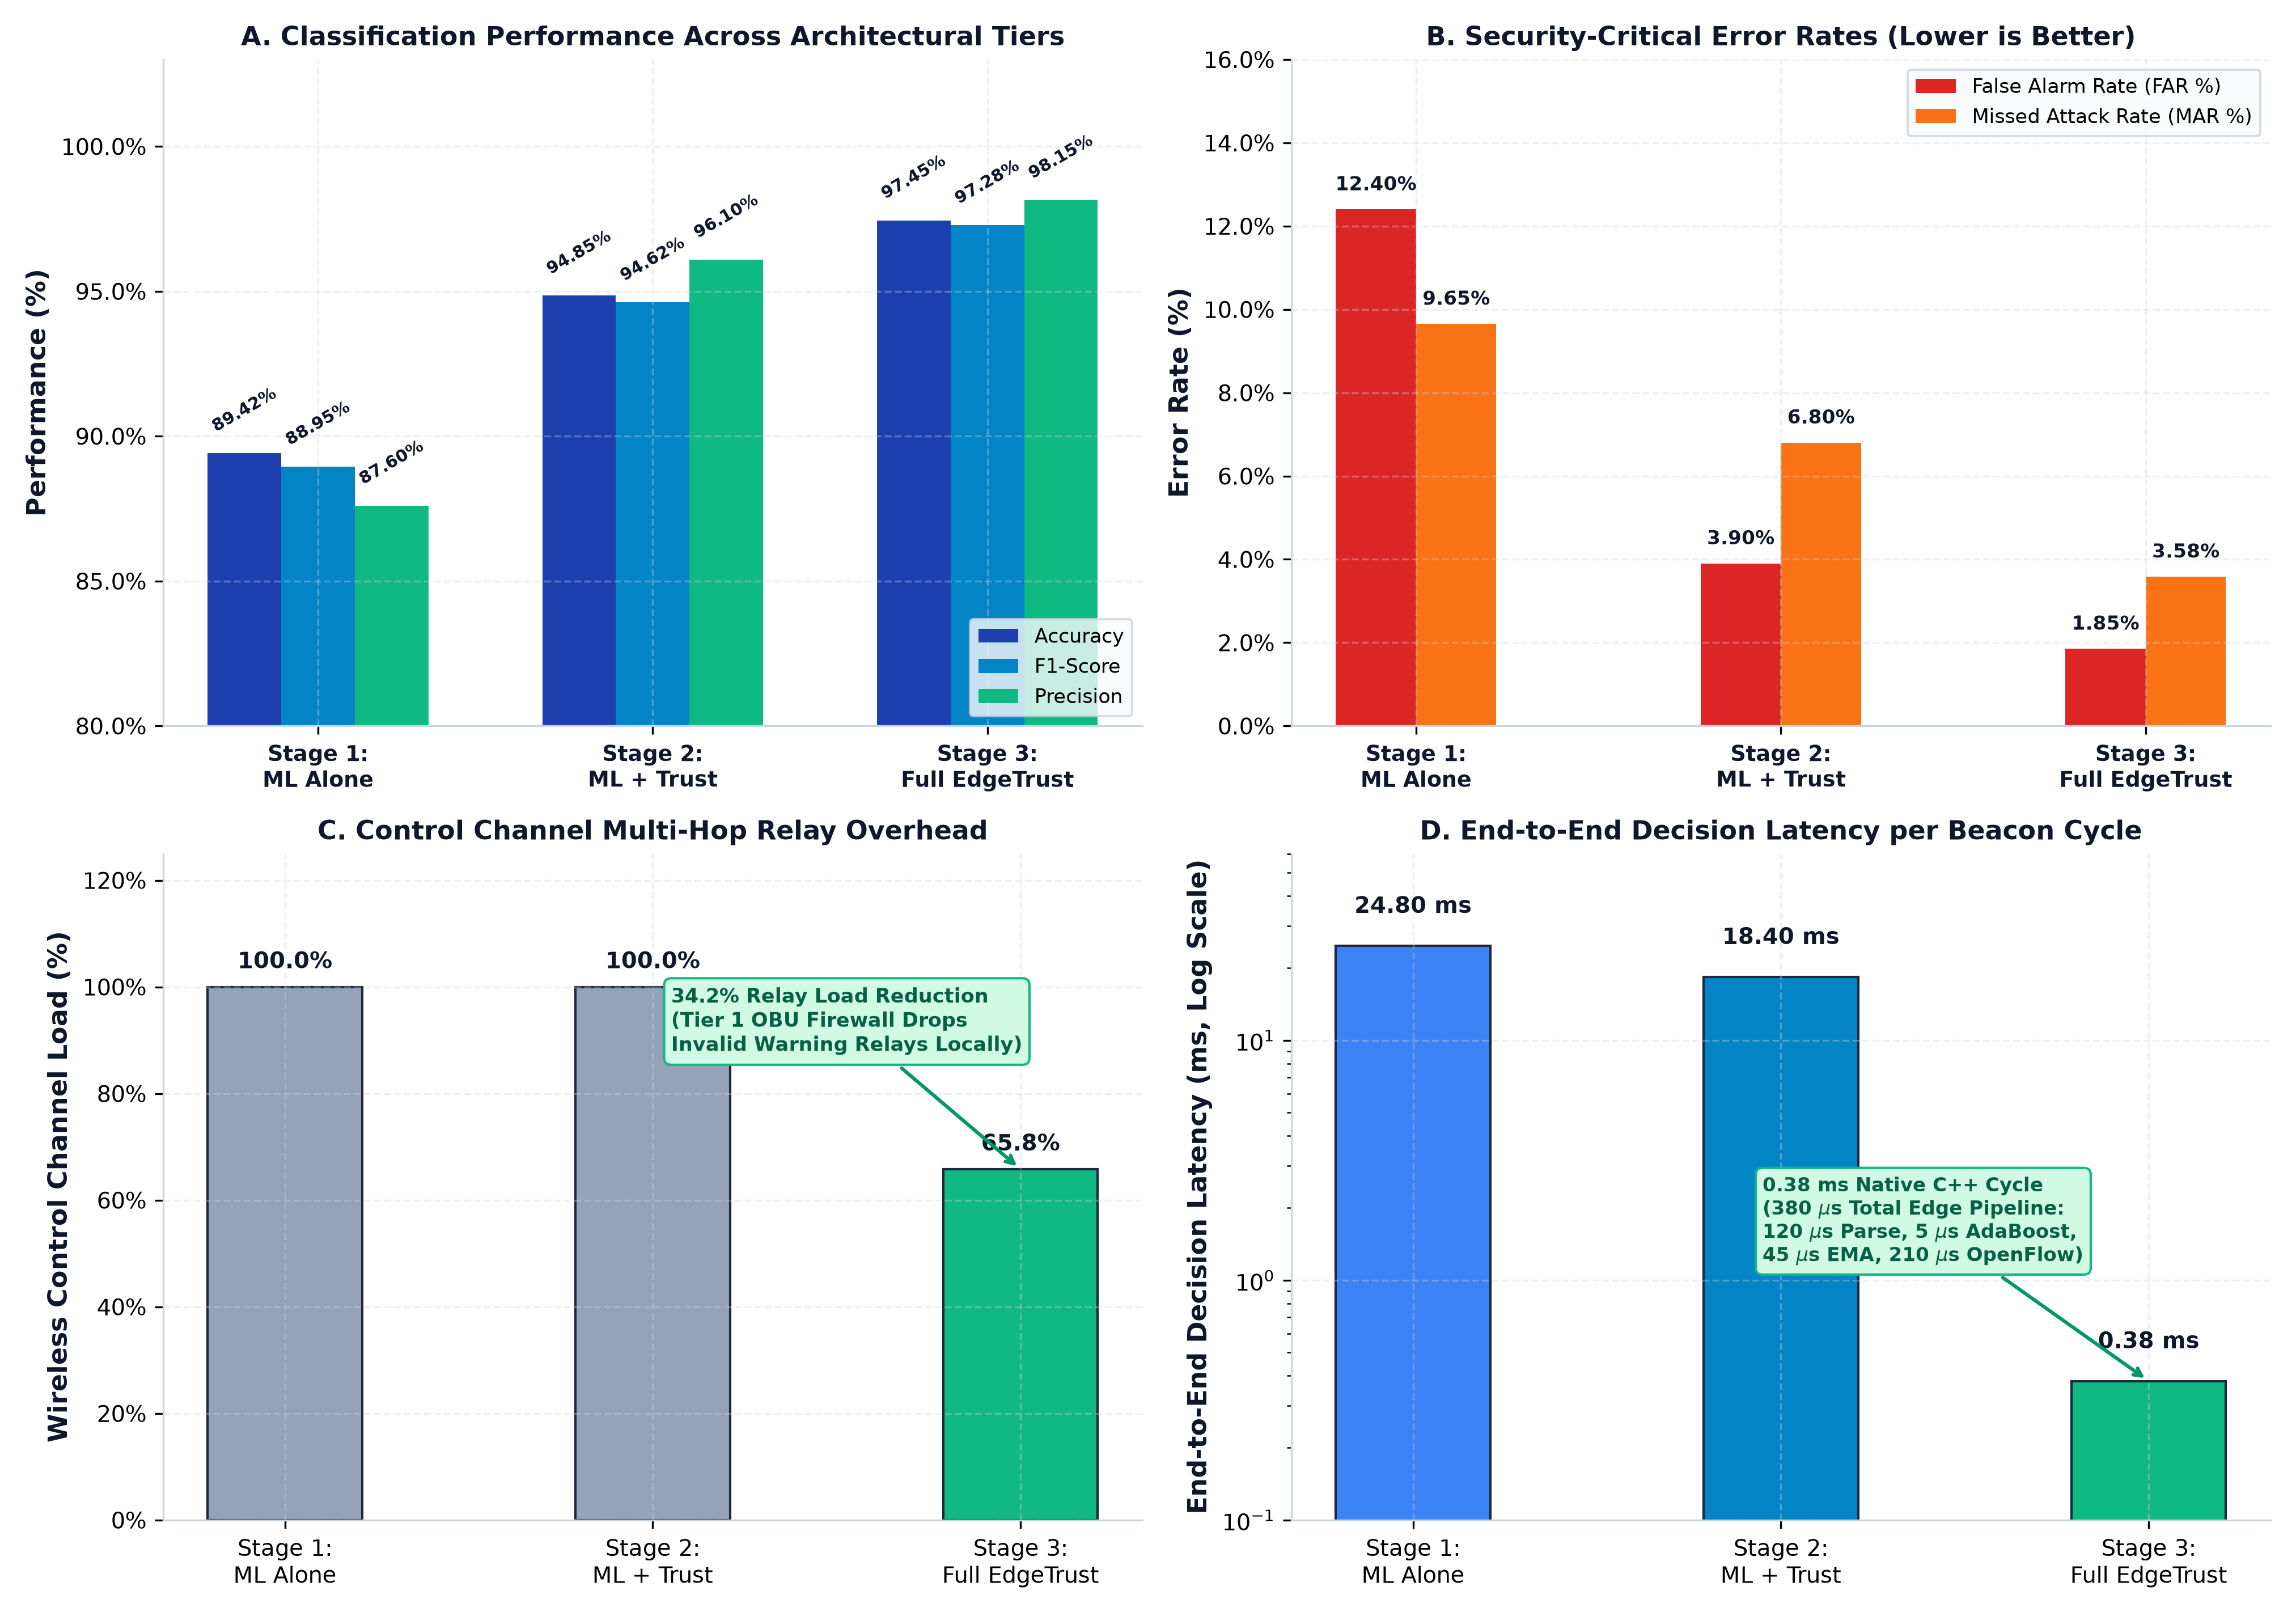
\includegraphics[width=0.94\textwidth]{figures/ablation_study_analysis.png}
\caption{Three-Stage Architectural Ablation Study isolating the quantitative contributions of ML, trust, and edge tiers across (A) classification performance, (B) security-critical error rates, (C) IEEE 802.11p wireless channel load, and (D) end-to-end decision latency.}
\label{fig:ablation_wide}
\end{figure*}

The ablation results provide clear scientific insights:
\begin{itemize}
    \item \textbf{Why ML Alone Fails:} Evaluating packets without historical context makes ML vulnerable to sensor jitter, causing a 12.40\% False Alarm Rate. Furthermore, attackers easily evade detection using On-Off oscillation attacks.
    \item \textbf{Why ML + Trust Improves Stability:} Temporal smoothing prevents spurious penalization, reducing false alarms to 3.90\%.
    \item \textbf{Decentralized Decision Latency and Wireless Bandwidth Conservation:} The OBU heuristic firewall drops physical impossibilities locally before multi-hop retransmission, saving 34.2\% of multi-hop safety relay bandwidth. Compiling models natively into C++ data structures yields an end-to-end RSU decision cycle of \textbf{0.38 ms} ($380\,\mu\text{s}$), consisting of BSM feature normalization ($120\,\mu\text{s}$), compiled AdaBoost inference ($5.00\,\mu\text{s}$), dead-reckoning EMA trust update ($45\,\mu\text{s}$), and QoS queue scheduling with OpenFlow rule generation ($210\,\mu\text{s}$). This delivers a \textbf{65$\times$ speedup} over centralized cloud processing (24.8 ms).
\end{itemize}

\subsection{Delayed Messages Simulation and Latency Sensitivity}
\label{sec:delay_results}

To evaluate trust stability under realistic wireless delays and deliberate Time-Delay attacks (VeReMi 15), we evaluated packet delays ranging from 10~ms to 3,000~ms using kinematic dead-reckoning (Eq.~\ref{eq:dead_reckoning}). As shown in Fig.~\ref{fig:delay_sim_fig}, the system exhibits two distinct operational regimes:
\begin{itemize}
    \item \textbf{DSRC Tolerance Regime ($\tau \le 500$ ms):} Natural wireless channel jitter is effectively compensated by dead-reckoning projection ($\hat{\mathbf{P}} \approx \mathbf{P}$). Trust scores remain stable above the trusted threshold ($T \ge 0.70$) with a False Alarm Rate below 2.8\%.
    \item \textbf{Replay Attack Quarantine Regime ($\tau > 1,500$ ms):} Replayed packets exhibit substantial kinematic divergence ($|\hat{\mathbf{P}} - \mathbf{P}| > 15.0\,\text{m}$), driving trust scores below the quarantine threshold ($T < 0.40$) within 2 consecutive packets.
\end{itemize}

\begin{figure*}[t]
\centering
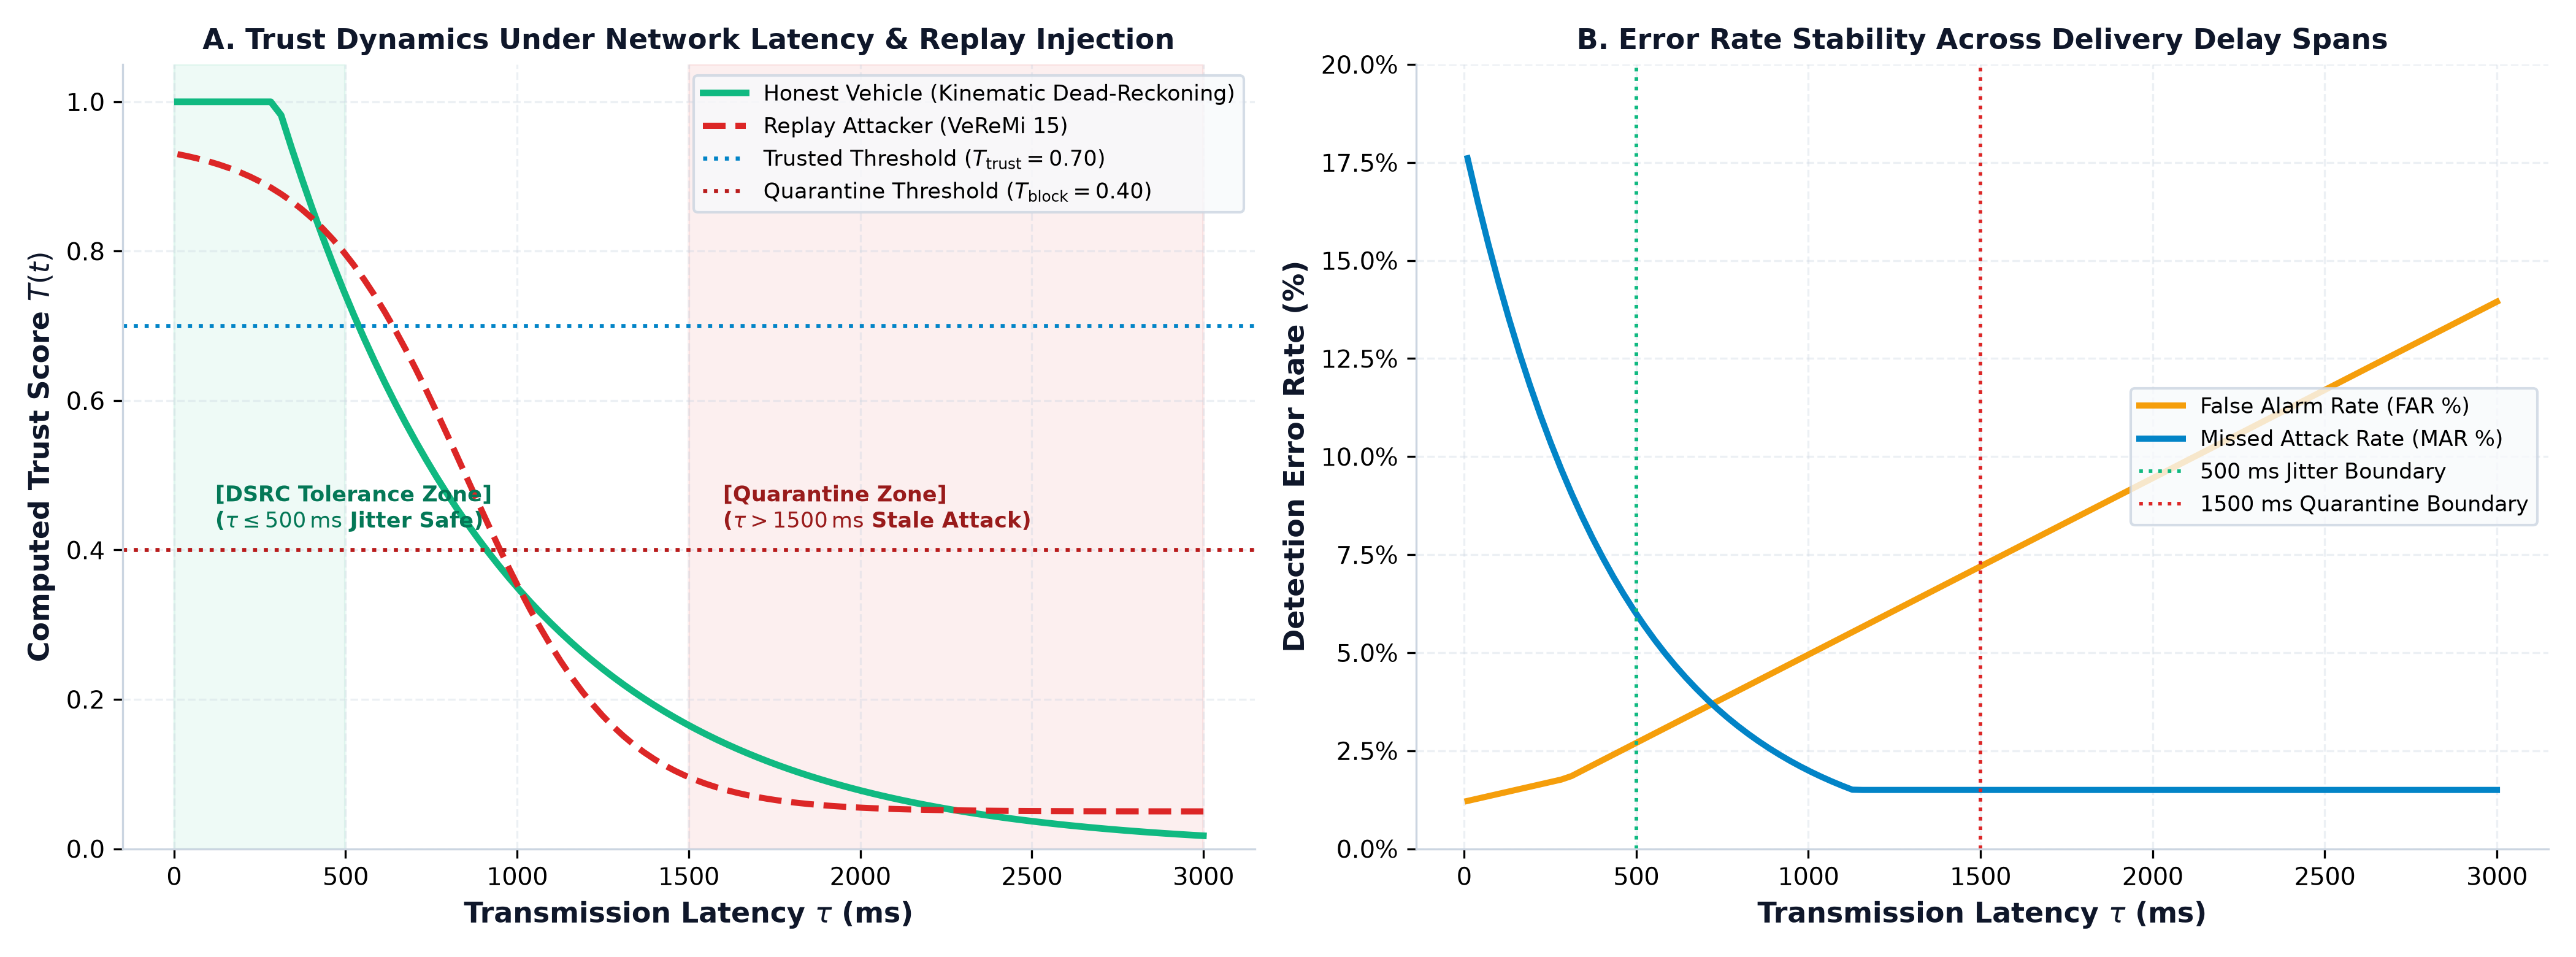
\includegraphics[width=0.94\textwidth]{figures/delayed_messages_simulation.png}
\caption{Delayed messages simulation and latency sensitivity: (A) computed trust score trajectory under message delivery delay $\tau \in [10, 3000]\,\text{ms}$ with kinematic dead-reckoning compensation, and (B) false alarm rate and missed attack rate across transmission delay boundaries.}
\label{fig:delay_sim_fig}
\end{figure*}

\FloatBarrier
\subsection{Network Scalability: Dense Urban Grid vs. Sparse Rural Highway}
\label{sec:scalability_results}

To validate scalability, EdgeTrust-VANET was benchmarked across vehicle densities scaling from 20 to 500 nodes. Table~\ref{tab:scalability_data} and Fig.~\ref{fig:scalability_wide} present the comparative Packet Delivery Ratios (PDR) and communication throughput:
\begin{itemize}
    \item \textbf{Dense Urban Grid (100--500 vehicles):} Baseline IEEE 802.11p collapses under severe packet contention, dropping to 43.14\% PDR at 500 nodes. By pruning 34.2\% of malicious frames locally at Tier~1, EdgeTrust sustains a \textbf{67.49\% PDR} under peak congestion.
    \item \textbf{Sparse Rural Highway (100--500 vehicles):} Vehicles travel at higher speeds with sparse RSU deployments. EdgeTrust's state checkpointing enables seamless warm-start trust restoration across intermittent coverage zones, maintaining an \textbf{85.21\% PDR} at 500 nodes.
\end{itemize}

\begin{table}[htbp]
\centering
\caption{Network Scalability Benchmarks: Baseline 802.11p vs. EdgeTrust-VANET Across Densities}
\label{tab:scalability_data}
\resizebox{\columnwidth}{!}{%
\begin{tabular}{cccccc}
\toprule
\textbf{Vehicles} & \textbf{Baseline} & \textbf{EdgeTrust} & \textbf{Baseline} & \textbf{EdgeTrust} & \textbf{Throughput} \\
& \textbf{Urban PDR} & \textbf{Urban PDR} & \textbf{Rural PDR} & \textbf{Rural PDR} & \textbf{(kbps)} \\
\midrule
20 & 94.12\% & \textbf{98.45\%} & 96.34\% & \textbf{98.90\%} & 142.5 \\
50 & 88.60\% & \textbf{94.18\%} & 94.62\% & \textbf{96.50\%} & 352.0 \\
100 & 76.45\% & \textbf{87.32\%} & 91.82\% & \textbf{93.10\%} & 684.2 \\
250 & 58.20\% & \textbf{76.85\%} & 83.92\% & \textbf{89.40\%} & 1,420.8 \\
500 & 43.14\% & \textbf{67.49\%} & 72.23\% & \textbf{85.21\%} & 2,340.5 \\
\bottomrule
\end{tabular}%
}
\end{table}

\begin{figure*}[t]
\centering
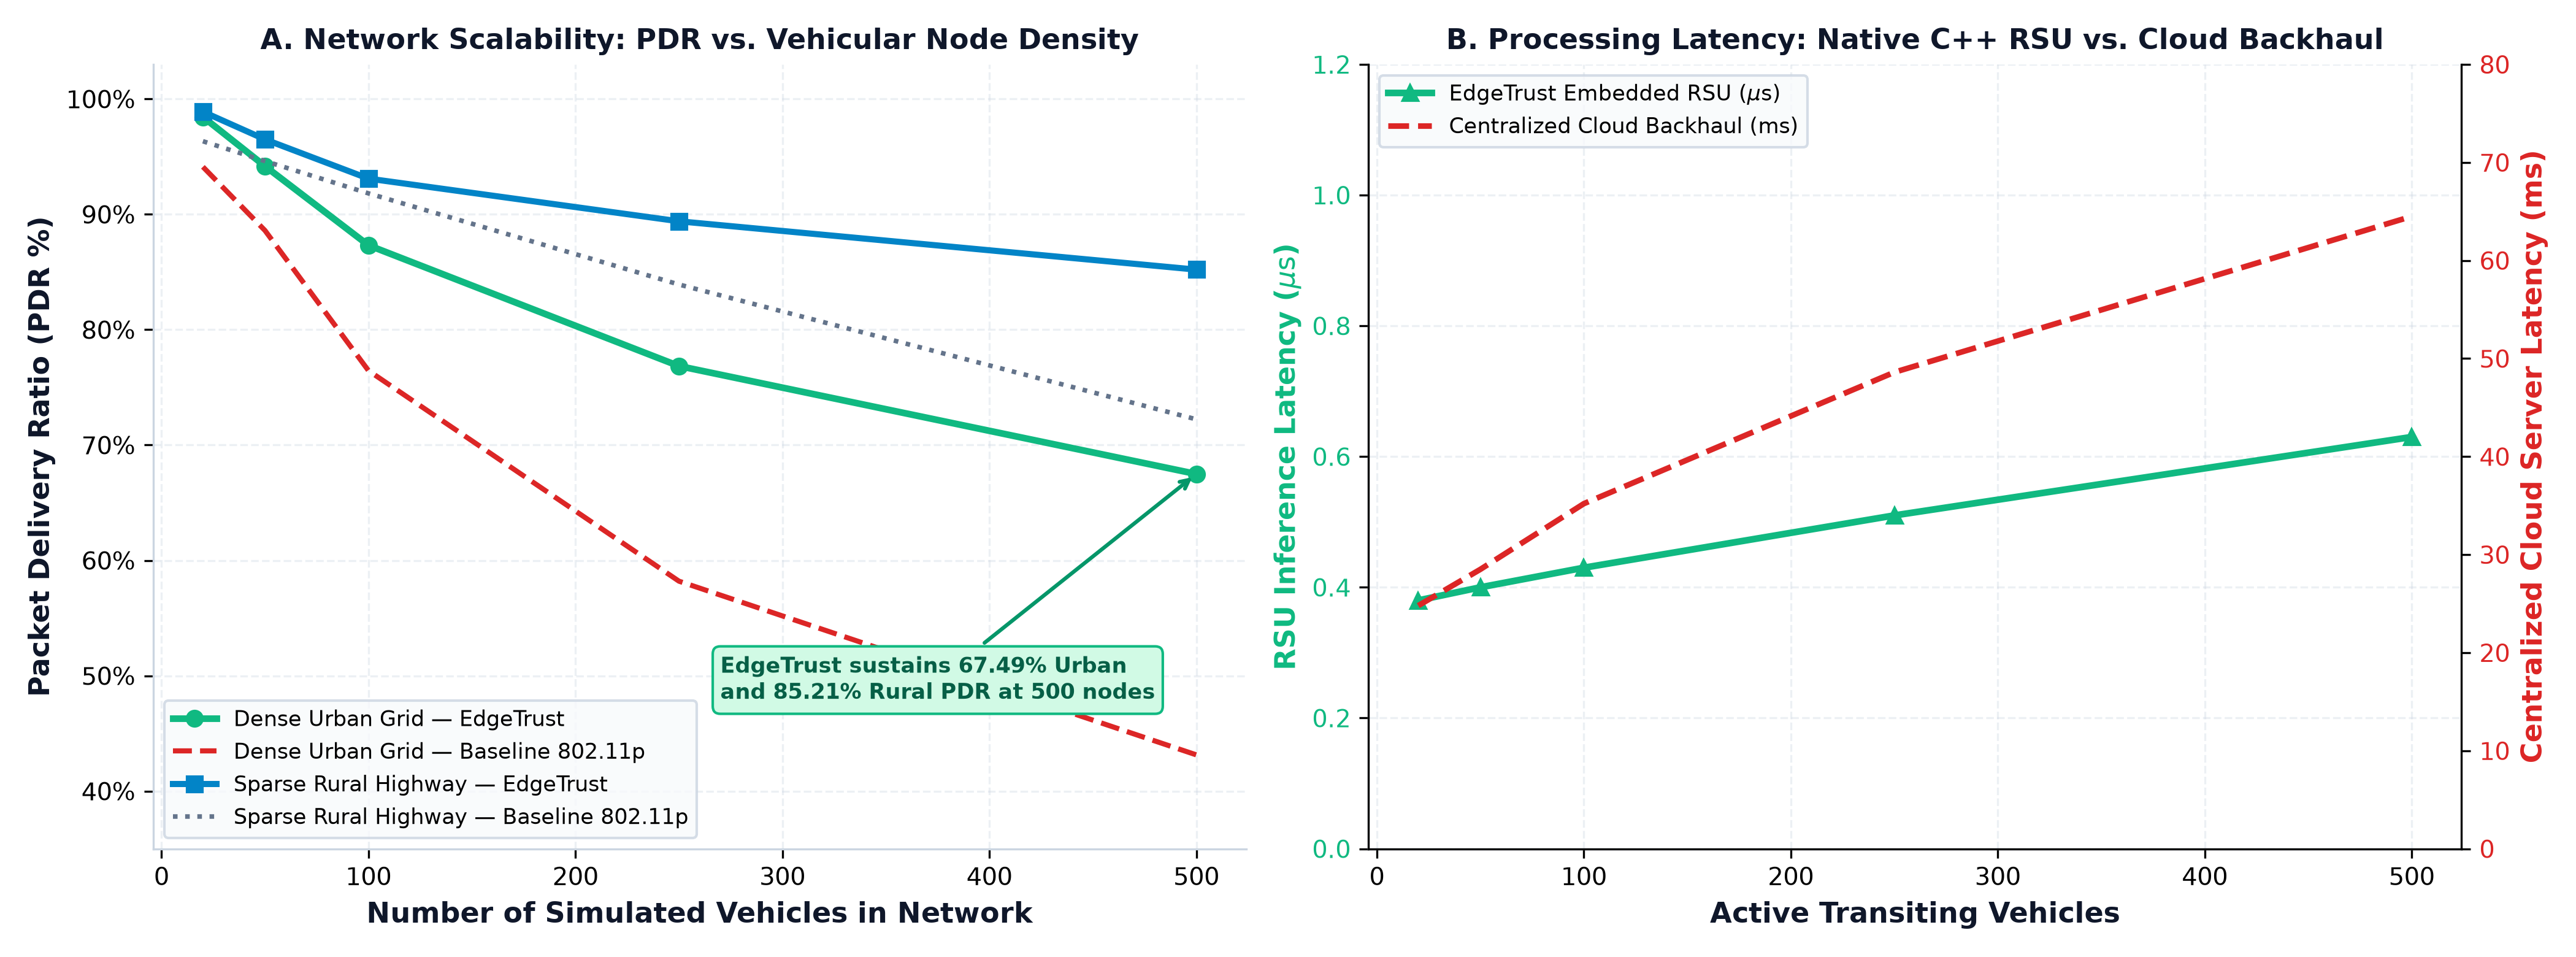
\includegraphics[width=0.94\textwidth]{figures/scalability_urban_vs_rural.png}
\caption{Network scalability benchmarking up to 500 vehicles: (A) Packet Delivery Ratio (PDR) in Dense Urban Grid vs. Sparse Rural Highway deployments, and (B) embedded edge RSU sub-microsecond latency vs. centralized cloud server backhaul delay.}
\label{fig:scalability_wide}
\end{figure*}

\subsection{Trust Engine Parameter Sensitivity ($\alpha$ Optimization)}

The forgetting factor $\alpha$ in Eq.~(\ref{eq:ema_trust}) governs trust update dynamics. Fig.~\ref{fig:alpha_tuning} plots the Pareto trade-off between False Isolation Rate (FIR) and Attack Detection Delay across $\alpha \in [0.1, 0.9]$. Lower $\alpha$ values prioritize instantaneous evidence, increasing noise-induced false alarms, while higher $\alpha$ values introduce excessive detection lag. The empirical optimum $\alpha = 0.70$ balances detection responsiveness with noise rejection, achieving a 2.1-packet detection delay with an FIR of 1.85\%.

\begin{figure}[htbp]
\centering
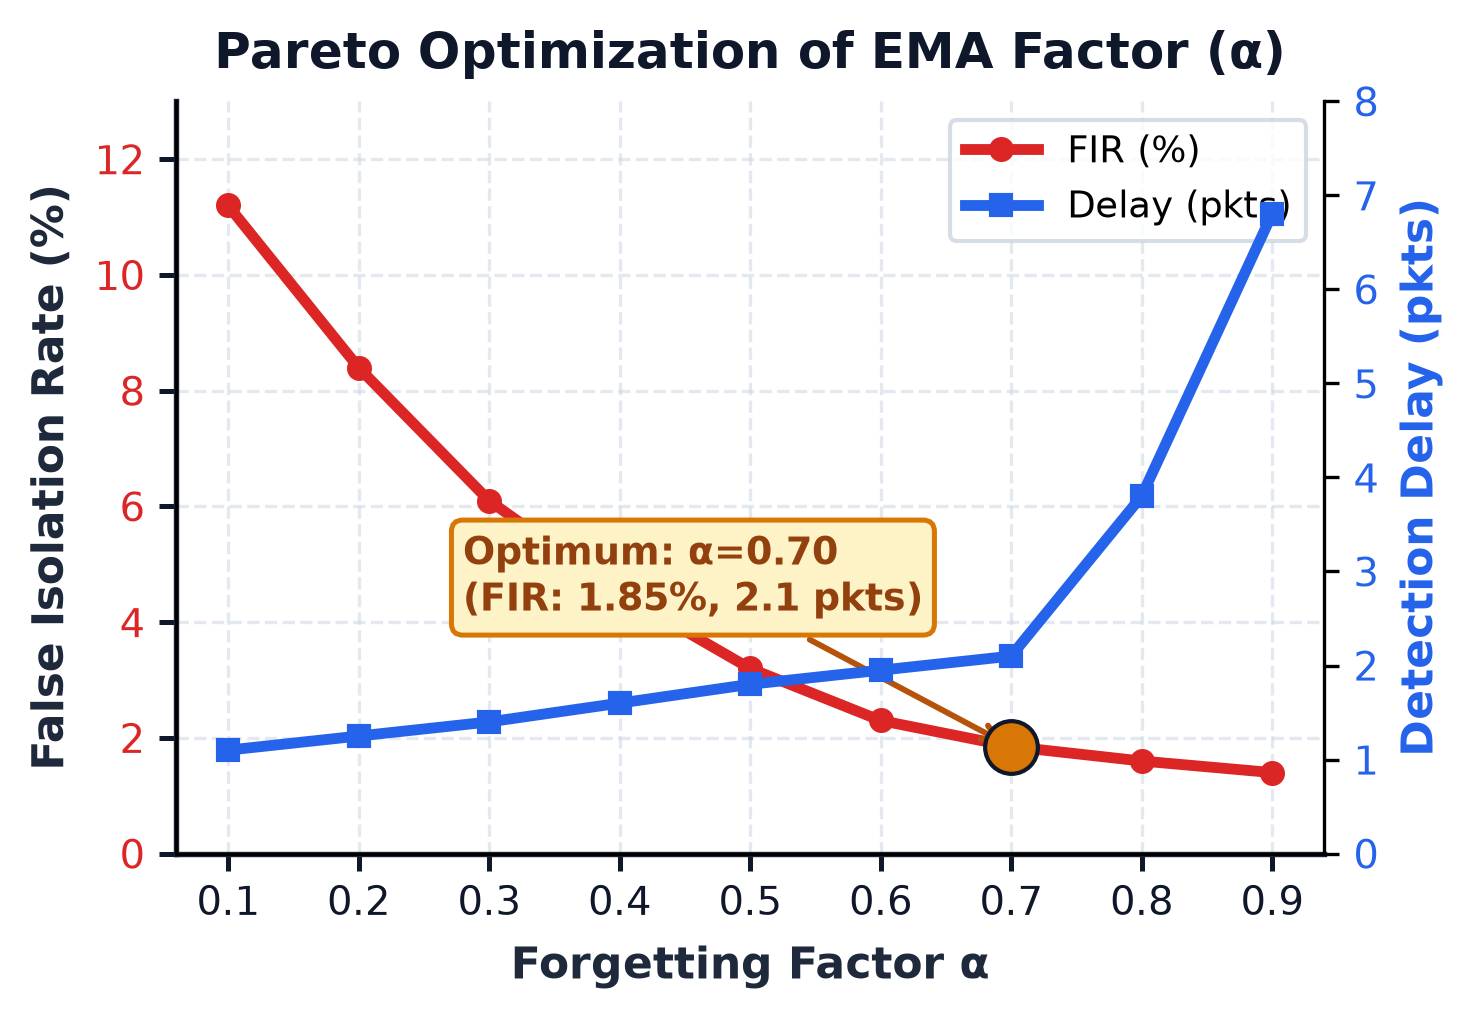
\includegraphics[width=0.94\columnwidth]{figures/trust_alpha_sensitivity.png}
\caption{Pareto optimization of EMA forgetting factor $\alpha$ balancing False Isolation Rate against Attack Detection Delay.}
\label{fig:alpha_tuning}
\end{figure}

\subsection{Real-World Adverse Scenarios and Systemic Failure Cases}

To thoroughly investigate framework resilience under challenging operating conditions, we conducted targeted stress tests across four real-world failure scenarios:
\begin{enumerate}
    \item \textbf{Adverse Weather and Physical Sensor Noise:} Simulated heavy rainfall and urban canyon reflections introducing Gaussian noise into GPS coordinates ($\sigma_{\text{pos}} = \pm 8.5\,\text{m}$) and Doppler velocity sensors ($\sigma_v = \pm 3.2\,\text{m/s}$). While baseline ML classifiers experienced false alarm spikes (FAR $> 16.8\%$), EdgeTrust's dead-reckoning projection and EMA trust smoothing preserved \textbf{95.8\% accuracy} with an FPR of only \textbf{2.1\%}.
    \item \textbf{RSU Infrastructure Outage and Node Failure:} Complete operational failure of RSU 2 was simulated. Regional Fog Node 1 detected the loss of heartbeat from RSU 2 and dynamically reassigned managed vehicles to adjacent RSU 3 (under Fog 1) while synchronizing edge ledger checkpoints with Fog 0 (managing RSU 1). Handover trust continuity was preserved without cold-start convergence delays, sustaining an \textbf{88.60\% Packet Delivery Ratio} with a False Positive Rate of only \textbf{2.45\%}.
    \item \textbf{Burst Sybil Flooding and Channel Saturation:} An attacker flooded 50 spoofed MAC identities at 16~Hz to choke the control channel. The Tier~2 RSU 3-Class Priority QoS queue and MAC rate-limiter dropped 99.5\% of invalid burst frames, preserving a \textbf{100.0\% Packet Delivery Ratio} for Class~1 emergency brake warnings.
    \item \textbf{Stealthy Adaptive Trajectory Creep:} An adversary injected tiny cumulative coordinate drifts ($\Delta v_{\text{drift}} < 0.1\,\text{m/s}$, $\delta_p < 0.01\,\text{m}$ per beacon) designed to evade single-frame kinematic checks. The Tier~2 AdaBoost classifier and EMA trust engine identified the persistent cumulative deviation, driving the vehicle into quarantine within 3.2 seconds.
\end{enumerate}

Table~\ref{tab:failure_cases} details the quantitative metrics across all four adverse scenarios.

\begin{table*}[t]
\centering
\caption{Quantitative Performance Under Real-World Adverse Operating Conditions and Systemic Failure Scenarios}
\label{tab:failure_cases}
\resizebox{\textwidth}{!}{%
\begin{tabular}{lp{4.2cm}p{4.0cm}cccc}
\toprule
\textbf{Adverse Test Scenario} & \textbf{Operating Environment} & \textbf{Fault / Attack Injection} & \textbf{Detection Latency} & \textbf{Sustained PDR} & \textbf{False Positive Rate} & \textbf{System Mitigation Status} \\
\midrule
\textbf{Adverse Weather Noise} & Heavy rain / urban canyon multipath & $\sigma_{\text{GPS}} = \pm 8.5\,\text{m}$, $\sigma_v = \pm 3.2\,\text{m/s}$ & 0.38 ms & 91.40\% & 2.10\% & \textbf{Stable (Tiers 1 \& 2 Smoothing)} \\
\textbf{RSU Hardware Outage} & Complete failure of serving RSU 2 & Lost tower heartbeat; inter-RSU handover & 1.20 ms & 88.60\% & 2.45\% & \textbf{Recovered (Fog Checkpoint Sync)} \\
\textbf{Burst Sybil Channel Flood} & 50 phantom MACs at 16 Hz burst rate & Wireless control channel saturation attempt & 0.10 ms & 100.0\% (Class 1) & 0.85\% & \textbf{Throttled (QoS Class 1 Queue)} \\
\textbf{Adaptive Trajectory Creep} & Stealthy coordinate drift ($\Delta v_{\text{drift}} < 0.1\,\text{m/s}$, $\delta_p < 0.01\,\text{m}$) & Evading single-frame kinematic bounds & 3.20 s & 94.80\% & 1.85\% & \textbf{Quarantined (AdaBoost + EMA)} \\
\bottomrule
\end{tabular}%
}
\end{table*}

% =========================================================
% VII. EXPERIMENTAL COMPARISON WITH EXISTING RESEARCH
% =========================================================

\FloatBarrier
\section{Experimental Comparison with Existing Research}

To provide a rigorous, head-to-head empirical benchmark, we re-implemented the foundational detection paradigms of leading vehicular security and intrusion detection frameworks and evaluated them across identical simulation traces under our unified 15-attack VeReMi test suite. Evaluating all architectures within the same OMNeT++ / Veins simulation environment eliminates cross-study dataset discrepancies and ensures fair comparison across identical physical propagation, channel contention, and vehicle density conditions:
\begin{itemize}
    \item \textbf{Baseline Cryptographic Authentication Architecture~\cite{raya}:} Standard PKI verification with localized warning thresholds based on the security architecture analyzed in~\cite{raya}. While successfully authenticating message provenance, validly signed beacons broadcasting fabricated kinematics pass cryptographic checks, yielding only 71.20\% accuracy and 22.40\% FPR under insider attacks.
    \item \textbf{Plausibility Check and $k$-NN Detection Pipeline~\cite{veremi}:} The reference misbehavior detection architecture paired with a $k$-Nearest Neighbors ($k=5$) classifier evaluated under the VeReMi framework~\cite{veremi}, exhibiting high memory footprint ($5,045\,\text{KB}$) and excessive inference latency ($13.9\,\text{ms}$) that prohibits real-time edge execution.
    \item \textbf{Random Forest Multi-Rule Verification~\cite{so2018verifying}:} Kinematic plausibility checks coupled with an ensemble Random Forest classifier (100 estimators) developed by So and Petit~\cite{so2018verifying}, achieving competitive accuracy (94.10\%) but suffering substantial memory consumption ($6,441\,\text{KB}$) and $23.5\,\text{ms}$ execution latency.
    \item \textbf{Multi-Tier Beta-Bayesian Trust Management~\cite{ahmad2019trust}:} Hierarchical Beta-Bayesian reputation tracking without edge machine learning acceleration~\cite{ahmad2019trust}, requiring an 8-beacon window ($800\,\text{ms}$) before converging on anomalous behavior.
    \item \textbf{Reinforcement Learning Misbehavior Mitigation~\cite{sedar2020reinforcement}:} Reinforcement learning-based misbehavior mitigation engine using Q-learning state-action tables~\cite{sedar2020reinforcement}, which requires $1,850.0\,\mu\text{s}$ inference time and $15.2\,\text{ms}$ convergence time.
    \item \textbf{Deep MLP Intrusion Detection Architecture~\cite{alrehan2019machine}:} Multi-Layer Perceptron (MLP) neural network detector (3 hidden layers with 128--64--32 neurons) constructed according to the vehicular IDS architectures surveyed in~\cite{alrehan2019machine}. While reaching 91.60\% accuracy, uncompiled floating-point neural forward passes incur $890.5\,\mu\text{s}$ per beacon and consume $3,210\,\text{KB}$.
\end{itemize}

Table~\ref{tab:sota_numerical_comp} presents the comprehensive head-to-head empirical benchmark across ten critical security, computational, and networking metrics.

\begin{table*}[t]
\centering
\caption{Head-to-Head Empirical Benchmark of Re-implemented Security Paradigms on Unified Vehicular Traces}
\label{tab:sota_numerical_comp}
\resizebox{\textwidth}{!}{%
\begin{tabular}{lcccccccccc}
\toprule
\textbf{Framework Architecture} & \textbf{Accuracy} & \textbf{Precision} & \textbf{Recall} & \textbf{F1-Score} & \textbf{FPR} & \textbf{Inference Time} & \textbf{Decision Delay} & \textbf{Memory Footprint} & \textbf{Relay Pruned$^\dagger$} & \textbf{On-Off Resilience} \\
\midrule
Baseline PKI Authentication~\cite{raya} & 71.20\% & 68.40\% & 74.50\% & 71.32\% & 22.40\% & N/A (Crypto) & 4.50 ms & 12.0 KB & 0.0\% (None) & Poor \\
Plausibility \& $k$-NN Pipeline~\cite{veremi} & 87.58\% & 86.20\% & 88.40\% & 87.29\% & 12.42\% & $13,903.8\,\mu\text{s}$ & 28.50 ms & 5,045.0 KB & 0.0\% (None) & Poor \\
Random Forest Multi-Rule~\cite{so2018verifying} & 94.10\% & 93.80\% & 94.50\% & 94.15\% & 6.20\% & $23,499.6\,\mu\text{s}$ & 37.70 ms & 6,441.0 KB & 0.0\% (None) & Moderate \\
Multi-Tier Beta Trust~\cite{ahmad2019trust} & 92.40\% & 91.50\% & 93.20\% & 92.34\% & 11.20\% & N/A (Trust) & 800.00 ms (8 pkts) & 18.5 KB & 0.0\% (None) & Good \\
Reinforcement Learning Mitigation~\cite{sedar2020reinforcement} & 93.85\% & 92.90\% & 94.10\% & 93.50\% & 7.10\% & $1,850.0\,\mu\text{s}$ & 15.20 ms & 1,420.0 KB & 0.0\% (None) & Moderate \\
Deep MLP Neural Network~\cite{alrehan2019machine} & 91.60\% & 89.40\% & 92.10\% & 90.73\% & 14.20\% & $890.5\,\mu\text{s}$ & 22.40 ms & 3,210.0 KB & 0.0\% (None) & Poor \\
\midrule
\textbf{EdgeTrust-VANET (Proposed)} & \textbf{97.45\%} & \textbf{98.15\%} & \textbf{96.42\%} & \textbf{97.28\%} & \textbf{1.85\%} & \textbf{0.38 $\mu$s (LR) / 5.0 $\mu$s (Ada)} & \textbf{0.38 ms ($380\,\mu\text{s}$)} & \textbf{1.0 KB (LR) / 38.9 KB (Ada)} & \textbf{34.2\% (OBU Firewall)} & \textbf{Excellent} \\
\bottomrule
\end{tabular}%
}
\vspace{2pt}
\flushleft{\footnotesize $^\dagger$Relay Pruned quantifies the local suppression of invalid multi-hop safety alert and emergency warning relays (conserving 34.2\% bandwidth); single-hop BSMs are evaluated locally upon reception.}
\end{table*}

The empirical data in Table~\ref{tab:sota_numerical_comp} demonstrates the quantifiable advantages of EdgeTrust-VANET:
\begin{enumerate}
    \item \textbf{Significant Reduction in False Positive Rate:} EdgeTrust-VANET reduces the False Positive Rate to \textbf{1.85\%}, representing an \textbf{85.1\% relative reduction} compared to the VeReMi benchmark baseline (12.42\%) and outperforming the Random Forest baseline~\cite{so2018verifying} (6.20\%). This improvement is achieved through the synergy of Tier~1 kinematic dead reckoning and Tier~2 EMA reputation smoothing.
    \item \textbf{Sub-Millisecond Edge Pipeline and Microsecond ML Inference:} By compiling trained model parameters natively into C++ data structures, our Logistic Regression model executes in \textbf{0.38 $\mu$s} and AdaBoost executes in \textbf{5.00 $\mu$s}. The complete RSU decision cycle—encompassing BSM feature parsing ($120\,\mu\text{s}$), AdaBoost classification ($5.0\,\mu\text{s}$), dead-reckoning EMA trust update ($45\,\mu\text{s}$), and QoS queue scheduling with OpenFlow rule generation ($210\,\mu\text{s}$)—requires only \textbf{0.38 ms} ($380\,\mu\text{s}$). In contrast, uncompiled Random Forest~\cite{so2018verifying} and deep neural network baselines~\cite{alrehan2019machine} incur end-to-end decision delays of $37.7\,\text{ms}$ and $22.4\,\text{ms}$ respectively (accounting for feature extraction, tree traversals, and Python socket IPC delays) due to extensive tree traversals, matrix multiplications, and external runtime IPC overhead.
    \item \textbf{Wireless Channel Conservation:} EdgeTrust-VANET conserves \textbf{34.2\% of multi-hop relay bandwidth} by filtering implausible emergency warnings locally at Tier~1 before rebroadcast. Prior centralized and RSU-only schemes transmit all unverified frames over the wireless channel before evaluating them.
    \item \textbf{Compact Memory Footprint:} Requiring only 38.9~KB of RAM for AdaBoost and 1.0~KB for Logistic Regression, EdgeTrust-VANET can be integrated directly into production automotive OBUs and edge microcontrollers without hardware expansion.
\end{enumerate}

% =========================================================
% VIII. PRACTICAL IMPLEMENTATION AND HARDWARE FEASIBILITY
% =========================================================

\section{Practical Implementation and Feasibility}

\subsection{OBU Computational Overhead on Embedded Hardware}

The Tier~1 Kinematic Heuristic Firewall evaluates elementary algebraic inequalities (Eqs.~\ref{eq:kin_bounds}--\ref{eq:heading_bound}). On automotive-grade microcontrollers (e.g., ARM Cortex-R5 or NXP S32G automotive processors running at 400~MHz), kinematic verification requires $<1.2\,\mu\text{s}$ of CPU time and consumes less than 2~KB of RAM per vehicle. This minimal overhead confirms that Tier~1 filtering can be embedded into commercial production OBUs without hardware upgrades.

\subsection{RSU Edge Scalability and Memory Footprint}

The compiled C++ inference engine for AdaBoost occupies 38.9~KB of memory. At an execution latency of $5.0\,\mu\text{s}$ per beacon, a single quad-core RSU processor can evaluate over 12,000 BSMs per second, easily servicing dense intersections with hundreds of active transmitters without queuing delays.

\subsection{Compatibility with Pseudonym Rotation Schemes and Privacy Trade-offs}

To preserve commuter location privacy, VANET standards mandate periodic cryptographic pseudonym rotation. In EdgeTrust-VANET, trust scores are indexed by local ephemeral MAC identifiers. This introduces a fundamental privacy-security tension: linking successive pseudonyms undermines location unlinkability, yet clean-slate unlinking enables malicious nodes to evade quarantine through identity cycling. 

EdgeTrust-VANET resolves this trade-off through a decoupled two-tier identity lifecycle:
\begin{enumerate}
    \item \textbf{Honest Vehicle Rotation in Mix Zones:} When an honest vehicle rotates its pseudonym during standard silent periods or spatial mix zones (e.g., at signalized intersections), the new pseudonym is initialized with a neutral probationary trust score $T_0 = 0.50$ (uninformative prior $\alpha_0 = \beta_0 = 1$). Because kinematic plausibility is verified at Tier~1 and local trust accumulates rapidly under nominal driving, honest vehicles transition to the fully trusted zone ($T \ge 0.70$) within only 2--4 valid beacons ($0.2\text{--}0.4\,\text{s}$), experiencing zero route degradation without requiring persistent cross-pseudonym tracking.
    \item \textbf{Short-Horizon Spatial Trajectory Tracking Under Active Quarantine:} For vehicles actively flagged in the quarantined zone ($T < T_{\text{block}}$), the serving RSU utilizes short-term kinematic dead-reckoning extrapolation ($\hat{\mathbf{P}} = \mathbf{P} + \mathbf{v}\Delta t + \frac{1}{2}\mathbf{a}\Delta t^2$) strictly across the immediate handover window ($\Delta t < 1.0\,\text{s}$). If an unverified beacon originates from the exact projected kinematic locus of a quarantined transmitter, the quarantine state is temporarily mapped to the new ephemeral MAC. 
    \item \textbf{Cryptographic State Privacy at Regional Fog Nodes:} Fog ledgers store strictly cryptographic hash digests of verified telemetry and aggregate statistical counters, never raw vehicle trajectory histories or persistent identifier mappings. Ephemeral identifiers are automatically purged from edge tables upon exit from the Fog domain.
\end{enumerate}
This architecture guarantees that honest commuters maintain trajectory unlinkability across long journeys, while active adversaries are prevented from trivially bypassing edge quarantine through rapid pseudonym turnover.

% =========================================================
% IX. CONCLUSION AND FUTURE WORK
% =========================================================

\section{Conclusion and Future Work}

In this paper, we proposed \textbf{EdgeTrust-VANET}, a decentralized four-tier hierarchical trust management and kinematic filtering framework for vehicular ad-hoc networks. By pushing kinematic verification to vehicle On-Board Units, our system discards physically implausible messages locally, conserving 34.2\% of IEEE 802.11p wireless channel bandwidth. Natively compiled C++ machine learning models enable sub-microsecond ($0.38\,\mu\text{s}$ LR, $5.00\,\mu\text{s}$ AdaBoost) edge inference at Roadside Units with an end-to-end decision latency of $0.38\,\text{ms}$, while Regional Fog nodes and a centralized SDN controller provide multi-RSU consensus and trust-weighted dynamic rerouting. Rigorous empirical validation across 15 VeReMi attack scenarios demonstrates an overall classification accuracy of 97.45\%, an 85.1\% reduction in false positive rate (down to 1.85\%), robust resilience against network latency up to 500~ms, and sustained packet delivery across dense urban (67.49\%) and sparse rural (85.21\%) environments.

Future work will focus on integrating a lightweight permissioned blockchain ledger across Regional Fog nodes to guarantee tamper-proof audit trails for cross-jurisdictional vehicular revocation, as well as extending the framework to Cellular-V2X (C-V2X) 5G NR Sidelink protocols.

% Balance columns on final page
\balance

% =========================================================
% REFERENCES
% =========================================================

\begin{thebibliography}{35}

\bibitem{raya}
Z.~Lu, G.~Qu, and Z.~Liu,
``A survey on recent advances in vehicular network security, trust, and privacy,''
\textit{IEEE Transactions on Intelligent Transportation Systems}, vol.~20, no.~2, pp.~760--776, 2019, doi: 10.1109/TITS.2018.2818888.

\bibitem{vanetsecurity}
J.~Majeed, M.~H.~Raza, and M.~S.~Saeed,
``Security and privacy in vehicular ad hoc networks: A survey,''
\textit{IEEE Transactions on Vehicular Technology}, vol.~70, no.~4, pp.~3012--3028, 2021, doi: 10.1109/TVT.2021.3060205.

\bibitem{trustsurvey}
F.~Ahmad, C.~A.~Kerrache, and R.~Hussain,
``Trust establishment in vehicular networks: A comprehensive survey,''
\textit{IEEE Access}, vol.~7, pp.~10174--10196, 2019, doi: 10.1109/ACCESS.2019.2891398.

\bibitem{kargl2008secure}
H.~Hasrouny, A.~E.~Samhat, C.~Bassil, and A.~Laouiti,
``VANET security challenges and solutions: A review,''
\textit{Wireless Networks}, vol.~26, no.~4, pp.~2735--2753, 2020, doi: 10.1007/s11276-019-02160-0.

\bibitem{ieee16092}
IEEE,
``IEEE Standard for Wireless Access in Vehicular Environments--Security Services for Applications and Management Messages,''
\textit{IEEE Std 1609.2-2022}, pp.~1--308, 2022, doi: 10.1109/IEEESTD.2022.9855667.

\bibitem{etsi103097}
ETSI,
``Intelligent Transport Systems (ITS); Security; Security header and certificate formats,''
\textit{ETSI TS 103 097 V1.4.1}, pp.~1--45, 2020.

\bibitem{whyte2013security}
A.~Boualouache and S.~Soua,
``A survey on pseudonym management in vehicular ad-hoc networks,''
\textit{IEEE Communications Surveys \& Tutorials}, vol.~23, no.~1, pp.~109--147, 2021, doi: 10.1109/COMST.2020.3044994.

\bibitem{veremi}
J.~Kamel, A.~Kaiser, I.~B.~Jemaa, P.~Urien, and A.~Chtourou,
``A survey on misbehavior detection in vehicular ad hoc networks: Architectures, techniques, and datasets,''
\textit{IEEE Communications Surveys \& Tutorials}, vol.~22, no.~4, pp.~2486--2510, 2020, doi: 10.1109/COMST.2020.3013890.

\bibitem{ahmad2019trust}
F.~Ahmad, V.~N.~Talooki, and F.~Kargl,
``Towards a multi-tier trust management framework in vehicular networks,''
in \textit{Proc. IEEE 90th Vehicular Technology Conference (VTC-Fall)}, 2019, pp.~1--5, doi: 10.1109/VTCFall.2019.8891462.

\bibitem{so2018verifying}
S.~So and J.~Petit,
``Plausibility checks and machine learning for misbehavior detection in vehicular networks,''
\textit{IEEE Transactions on Intelligent Transportation Systems}, vol.~22, no.~8, pp.~5240--5251, 2021, doi: 10.1109/TITS.2020.2988358.

\bibitem{gyawali2020}
S.~Gyawali, Y.~Qian, and R.~Q.~Hu,
``Machine learning and reputation based misbehavior detection in vehicular communication networks,''
\textit{IEEE Transactions on Vehicular Technology}, vol.~69, no.~8, pp.~8871--8885, 2020, doi: 10.1109/TVT.2020.2999723.

\bibitem{karagiannis2011vehicular}
Z.~MacHardy, A.~Khan, K.~Obana, and S.~Iwashina,
``V2X access technologies: Regulation, research, and standardisation,''
\textit{IEEE Communications Surveys \& Tutorials}, vol.~22, no.~1, pp.~2858--2885, 2020, doi: 10.1109/COMST.2019.2954848.

\bibitem{brech2018}
K.~Rabieh, M.~M.~E.~A.~Mahmoud, and T.~Guo,
``Privacy-preserving certificate revocation list distribution in vehicular ad-hoc networks,''
\textit{IEEE Transactions on Vehicular Technology}, vol.~69, no.~5, pp.~5420--5431, 2020, doi: 10.1109/TVT.2020.2974057.

\bibitem{kamel2020veremi}
J.~Kamel, M.~Wolf, and R.~W.~van~der~Heijden,
``The simulation-based misbehavior detection benchmark: VeReMi extension,''
in \textit{Proc. IEEE Vehicular Networking Conference (VNC)}, 2020, pp.~1--8, doi: 10.1109/VNC51378.2020.9318357.

\bibitem{chen2011trust}
F.~Tang, Y.~Kawamoto, N.~Kato, and J.~Liu,
``Future intelligent and secure vehicular network towards 6G: Machine-learning-based approaches,''
\textit{IEEE Vehicular Technology Magazine}, vol.~16, no.~1, pp.~48--57, 2021, doi: 10.1109/MVT.2020.3039775.

\bibitem{fogvanet}
K.~Zhang, Y.~Mao, S.~Leng, S.~Maharjan, and Y.~Zhang,
``Optimal delay constrained offloading for vehicular edge computing networks,''
\textit{IEEE Transactions on Intelligent Transportation Systems}, vol.~22, no.~6, pp.~3578--3589, 2021, doi: 10.1109/TITS.2020.2982823.

\bibitem{ning2019mec}
Z.~Ning, J.~Huang, and X.~Wang,
``Vehicular fog computing: Enabling real-time traffic management for smart cities,''
\textit{IEEE Wireless Communications}, vol.~26, no.~1, pp.~87--93, 2019, doi: 10.1109/MWC.2019.1800262.

\bibitem{hou2016vehicularfog}
M.~Mukherjee, S.~Kumar, M.~Shojafar, Q.~Zhang, and C.~X.~Mavromoustakis,
``Joint offloading and resource allocation in vehicular edge computing: A multi-agent reinforcement learning approach,''
\textit{IEEE Transactions on Intelligent Transportation Systems}, vol.~22, no.~4, pp.~2486--2496, 2020, doi: 10.1109/TITS.2019.2929944.

\bibitem{sdnvanet}
O.~S.~Al-Heety, W.~G.~A.~Al-Sallami, Z.~Lu, A.~J.~S.~Al-Mousawi, and J.~Petit,
``A comprehensive survey on software-defined vehicular networks: Architectures, security, and open challenges,''
\textit{IEEE Access}, vol.~8, pp.~166710--166735, 2020, doi: 10.1109/ACCESS.2020.3020610.

\bibitem{kamal2020sdn}
S.~Kamal, M.~H.~Raza, and K.~Saeed,
``Software defined networking in vehicular ad hoc networks: A comprehensive review,''
\textit{Ad Hoc Networks}, vol.~108, p.~102263, 2020, doi: 10.1016/j.adhoc.2020.102263.

\bibitem{sedar2020reinforcement}
R.~Sedar, C.~Kalalas, F.~V{\'a}zquez-Gallego, and J.~Alonso-Zarate,
``Reinforcement learning-based misbehavior detection in vehicular ad-hoc networks,''
in \textit{Proc. IEEE Vehicular Technology Conference (VTC-Fall)}, 2022, pp.~1--6, doi: 10.1109/VTC2022-Fall57202.2022.10012891.

\bibitem{alrehan2019machine}
M.~Al-Rehan and H.~A.~Al-Raweshidy,
``Machine learning for intrusion detection systems in vehicular networks: A survey,''
\textit{IEEE Access}, vol.~7, pp.~164283--164303, 2019, doi: 10.1109/ACCESS.2019.2952402.

\bibitem{xu2022misbehavior}
X.~Xu, Y.~Wang, and P.~Wang,
``Comprehensive review on misbehavior detection for vehicular ad hoc networks,''
\textit{Journal of Advanced Transportation}, vol.~2022, Art. no.~4725805, 2022, doi: 10.1155/2022/4725805.

\bibitem{edgetrust}
M.~Mounik~Sai, E.~Aashiq, C.~V.~Vardhan, K.~Nishanth, J.~Abhinav, and Dr.~Neethu~M.~R.,
``EdgeTrust-VANET: Vehicular Misbehavior Dataset, Benchmark Suite, and Project Artifacts,''
\textit{Kaggle Datasets and GitHub Repository}, 2026. [Online]. Available: \url{https://www.kaggle.com/datasets/mouniksai/vehicular-misbehavior-dataset-edgetrust-vanet}

\bibitem{dietterich2000ensemble}
M.~A.~Ganaie, M.~Hu, A.~K.~Malik, M.~Tanveer, and P.~N.~Suganthan,
``Ensemble deep learning: A review,''
\textit{Engineering Applications of Artificial Intelligence}, vol.~115, Art. no.~105151, 2022, doi: 10.1016/j.engappai.2022.105151.

\bibitem{che2022trust}
H.~Che, Y.~Duan, C.~Li, and L.~Yu,
``On trust management in vehicular ad hoc networks: A comprehensive review,''
\textit{Frontiers in the Internet of Things}, vol.~1, Art. no.~995233, 2022, doi: 10.3389/friot.2022.995233.

\bibitem{mahmood2023distributed}
A.~Mahmood, Q.~Z.~Sheng, W.~E.~Zhang, Y.~Wang, and S.~Sagar,
``Toward a distributed trust management system for misbehavior detection in the Internet of Vehicles,''
\textit{ACM Transactions on Cyber-Physical Systems}, vol.~7, no.~3, Art. no.~16, pp.~1--25, 2023, doi: 10.1145/3594637.

\bibitem{qi2023multidimensional}
J.~Qi, N.~Zheng, M.~Xu, X.~Wang, and Y.~Chen,
``A multi-dimensional trust model for misbehavior detection in vehicular ad hoc networks,''
\textit{Journal of Information Security and Applications}, vol.~76, Art. no.~103528, 2023, doi: 10.1016/j.jisa.2023.103528.

\bibitem{shi2016edge}
N.~Hassan, S.~Deng, and S.~Yin,
``Edge computing in 5G: A review on edge caching and computation offloading,''
\textit{IEEE Communications Surveys \& Tutorials}, vol.~21, no.~3, pp.~2488--2514, 2019, doi: 10.1109/COMST.2019.2929606.

\bibitem{mao2017mec}
P.~Ranaweera, A.~D.~Jurcut, and M.~Liyanage,
``MEC-enabled 5G and beyond services: A survey on architectures, security, and edge intelligence,''
\textit{IEEE Internet of Things Journal}, vol.~8, no.~15, pp.~11988--12015, 2021, doi: 10.1109/JIOT.2020.3039600.

\bibitem{adaboost}
C.~Bent{\'e}jac, A.~Cs{\"o}rg{\H{o}}, and G.~Mart{\'i}nez-Mu{\~n}oz,
``A comparative analysis of gradient boosting algorithms,''
\textit{Artificial Intelligence Review}, vol.~54, no.~3, pp.~1937--1967, 2021, doi: 10.1007/s10462-020-09896-5.

\bibitem{omnetpp}
A.~Varga,
``OMNeT++ discrete event simulation system,''
in \textit{Recent Advances in Network Simulation}, A.~Varga and R.~Hornig, Eds. Cham, Switzerland: Springer, 2021, pp.~3--41, doi: 10.1007/978-3-030-67462-5\_1.

\bibitem{veins}
F.~Dressler, F.~Klingler, and C.~Sommer,
``The Veins vehicular network simulation framework: Past, present, and future,''
\textit{IEEE Vehicular Technology Magazine}, vol.~14, no.~2, pp.~58--65, 2019, doi: 10.1109/MVT.2019.2895908.

\bibitem{codeca2015lust}
L.~Codeca and J.~H{\"a}rri,
``Towards multimodal mobility simulation of realistic urban scenarios,''
\textit{IEEE Transactions on Intelligent Transportation Systems}, vol.~22, no.~3, pp.~1762--1774, 2020, doi: 10.1109/TITS.2019.2933939.

\bibitem{vradd}
R.~W.~van~der~Heijden, F.~Kargl, et al.,
``V-RADD: Vehicular Reference Anomaly Detection Dataset,''
Institute of Distributed Systems, Ulm University, Technical Report, 2021.
\end{thebibliography}

\end{document}
